%% -*- coding:utf-8 -*-

\chapter{构式语法}
%\chapter{Construction Grammar}
\label{Kapitel-CxG}

% URL: fcg-net.
% Loreto Steels 2007 Emergence of language Nature Physics 3 (11) 758-760
%
% Vanessas Grammatik: wh-Fragen mit allen Fragepronomina, aber keine Fernabhängigkeit
% Deklarative Sätze nur mit Subjekt im VF
%
%
% Bybee2006:713
%
% 2002). Erman and Warren (2000) found that what they call prefabricated word combinations
% constitute about 55% of both spoken and written discourse. Speakers recognize prefabs as familiar,
% which indicates that these sequences of words are stored in memory despite being largely
% predictable in form and meaning.

与LFG和HPSG一样,构式语法(Construction Grammar\isc{构式语法(CxG)|(}\is{Construction Grammar (CxG)|(},简称为CxG)也是西海岸语言学的一部分。它深受Charles Fillmore、Paul Kay、George Lakoff(他们三人都在伯克利大学)和Adele Goldberg(她在伯克利大学完成了自己的博士学位,现在在普林斯顿大学工作)\citep*{Fillmore88a,FKoC88a,KF99a,Kay2002a,Kay2005a,Goldberg95a,Goldberg2006a}的影响。
%Like LFG and HPSG, \emph{Construction Grammar}\is{Construction Grammar (CxG)|(} (CxG) forms part of West Coast linguistics.
%It has been influenced considerably by Charles Fillmore, Paul Kay and George Lakoff (all three at Berkeley) and Adele Goldberg
%(who completed her PhD in Berkeley and is now in Princeton)
%\citep*{Fillmore88a,FKoC88a,KF99a,Kay2002a,Kay2005a,Goldberg95a,Goldberg2006a}.

Fillmore、Kay、Jackendoff以及其他学者都指出:在很大程度上,语言包括无法用现有工具进行直接描写的复杂单位。在类似于GB理论这样的理论框架中,将核心语法\isc{核心语法}\is{core grammar}和边缘现象\isc{边缘现象}\is{periphery}作明确区分\citep[\page 8]{Chomsky81a},并且在构建一种普遍语法理论的时候,边缘现象几乎被认为是没有研究价值的。构式语法对于这一做法的批评是有理据的,因为什么是“边缘现象”有时候看起来是完全随意的\citep{MuellerKernigkeit},并且仅仅因其在某种程度上是不规则的就将很多语言现象排除在外并不会在理论建设上取得进步。
%Fillmore, Kay, Jackendoff and others have pointed out the fact that, to a large extent, languages consist of complex units that cannot straightforwardly
%be described with the tools that we have seen thus far. In frameworks such as GB, an explicit distinction is made between core grammar\is{core grammar}
%and the periphery\is{periphery} \citep[\page 8]{Chomsky81a}, whereby the periphery is mostly disregarded as uninteresting when formulating a theory
%of Universal Grammar. The criticism leveled at such practices by CxG is justified since what counts as the `periphery' sometimes seems completely
%arbitrary \citep{MuellerKernigkeit} and no progress is made by excluding large parts of the language
%from the theory just because they are irregular to a certain extent.

构式语法经常讨论熟语表达与常规表达之间的互动关系。 \citet{KF99a}在他们的经典论文中研究了What's X doing Y?"=构式。(\mex{1})包含这一构式的一些实例:
%In Construction Grammar, idiomatic expressions are often discussed with regard to their interaction
%with regular areas of grammar.  \citet{KF99a} studied the \emph{What's X doing Y?}"=construction in
%their classic essay. (\mex{1}) contains some examples of this construction: 
\eal
\ex 
\gll What is this scratch doing on the table?\\
      什么 \textsc{aux} 这 擦痕 做 \textsc{prep} \textsc{det} 桌子\\
\mytrans{桌子上为什么有擦痕?}
\ex 
\gll What do you think your name is doing in my book?\\
      什么 \textsc{aux} 你 想 你的 名字 \textsc{aux} 做 \textsc{prep} 我的 书\\
\mytrans{你觉得我书上为什么有你的名字?}
%\ex What is this scratch doing on the table?
%\ex What do you think your name is doing in my book?
\zl
这些例子表明该构式中do的意义不是其常规意义。在该构式中,do除了涉及语义淡化(semantic bleaching)之外,还必须满足特定的形态句法限制。动词do必须要出现,且以现在分词的形式出现。Kay和Fillmore分析了该构式,找到了WXDY"=构式与语法中其他构式之间的共同点。
%The examples show that we are clearly not dealing with the normal meaning of the verb \emph{do}. As well as the semantic bleaching here,
%there are particular morphosyntactic properties that have to be satisfied in this construction. The verb \emph{do} must always be present
%and also in the form of the present participle. Kay and Fillmore develop an analysis explaining this construction and also capturing some
%of the similarities between the WXDY"=construction and the rest of the grammar.
构式语法的变体有很多,主要有:
%There are a number of variants of Construction Grammar:
\begin{sloppypar}
\begin{itemize}
\item 伯克利构式语法 \citep{Fillmore88a,KF99a,FriedHSK}
\item Goldberg/Lakoff的构式语法 \citep{Lakoff87a-u,Goldberg95a,Goldberg2006a}
\item 认知语法\isc{认知语法}\is{Cognitive Grammar} \citep{Langacker87a-u,Langacker2000a,Langacker2008a-u,Dabrowska2004a}
\item 激进构式语法 \citep{Croft2001a}
\item 体验构式语法 \citep{BC2005a}
\item 动变构式语法 \citep{SDB2006a-u,SteelsFluid-ed-not-crossreferenced}
\item 基于符号的构式语法 \citep{Sag2010b,Sag2012a}
%\item Berkeley Construction Grammar \citep{Fillmore88a,KF99a,FriedHSK}
%\item Goldbergian/Lakovian Construction Grammar \citep{Lakoff87a-u,Goldberg95a,Goldberg2006a}
%\item Cognitive Grammar\is{Cognitive Grammar} \citep{Langacker87a-u,Langacker2000a,Langacker2008a-u,Dabrowska2004a}
%\item Radical Construction Grammar \citep{Croft2001a}
%\item Embodied Construction Grammar \citep{BC2005a}
%\item Fluid Construction Grammar \citep{SDB2006a-u,SteelsFluid-ed-not-crossreferenced}
%\item Sign-Based Construction Grammar \citep{Sag2010b,Sag2012a}
\end{itemize}
\end{sloppypar}

\noindent
构式语法的目标既全面描写语言,也在理论上探索语言。但是,实际上相比于GB理论中被描述为“核心语法”的现象,构式语法给予不规则现象更多的关注。构式语法经常将语言现象分析为短语模式。这些短语模式被表征为承继层级(\egc \citealp{Croft2001a,Goldberg2003a})。短语构式假设的一个例子就是Goldberg对于动结构式\isc{构式!动结构式}\is{construction!resultative}的分析。 \citet{Goldberg95a}和 \citet{GJ2004a}主张动结式是构式。按照他们的观点,例(\mex{1})中没有能够确定论元数量的中心语。
%The aim of Construction Grammar is to both describe and theoretically explore language in its entirety.
%In practice, however, irregularities in language are often given far more importance than the phenomena described
%as `core grammar' in GB. Construction Grammar analyses usually analyze phenomena as phrasal patterns.
%These phrasal patterns are represented in inheritance hierarchies (\eg \citealp{Croft2001a,Goldberg2003a}).
%
%An example for the assumption of a phrasal construction is Goldberg's analysis of resultative constructions\is{construction!resultative}.
% \citet{Goldberg95a} and  \citet{GJ2004a} argue for the construction status of resultatives. In their view, there is no head
%in (\mex{1}) that determines the number of arguments.
\ea
\gll Willy watered the plants flat.\\
	 Willy 浇水 \textsc{det} 植物 平\\
\mytrans{Willy浇水把植物浇平了。}
%Willy watered the plants flat.
\z
相反,论元的数量由构式决定,也就是说,一个规则或者程式。这一规则或模式规定,主语、动词、宾语和一个述谓成分必须出现在一起并且整个复杂体(complex)有一定特定的意义。这一观点与GB理论\indexgbc(GB)、范畴语法\indexcgc(Categorial Grammar)、词汇功能语法\footnote{参看 \citew{Alsina96a}和 \citew*{ADT2008a,ADT2013a}。关于这一点更多的讨论参看\ref{sec-aspect-at-clause-level}和\ref{sec-phrasal-LI}。%
}\indexlfgc(LFG)和中心词驱动的短语结构语法\indexhpsgc(HPSG)中的分析有根本上的不同。在前述理论中,都假定论元是由词汇中心语选择的而不是由短语规则独立允准的。可以参看 \citew{Simpson83a},  \citew{Neeleman94a},  \citew{Wunderlich97c},  \citew{Wechsler97a}和 \citew{Mueller2002b}在LFG、GB中做的相应工作,Wunderlich的词汇分解语法\aimention{Dieter Wunderlich}\isc{词汇分解语法}\is{Lexical Decomposition Grammar}和HPSG的工作。
%The number of arguments is determined by the construction instead, that is, by a rule or schema saying that the subject, verb, object and a predicative
%element must occur together and that the entire complex has a particular meaning. This view is fundamentally different from analyses in GB\indexgb,
%Categorial Grammar\indexcg, LFG\footnote{%
%	See  \citew{Alsina96a} and  \citew*{ADT2008a,ADT2013a}, however. For more discussion of this point, see
%        Sections~\ref{sec-aspect-at-clause-level} and~\ref{sec-phrasal-LI}.%
%}\indexlfg and HPSG\indexhpsg.
%In the aforementioned theories, it is commonly assumed that arguments are always selected by lexical heads and not independently licensed by phrasal
%rules. See  \citew{Simpson83a},  \citew{Neeleman94a},  \citew{Wunderlich97c},  \citew{Wechsler97a}, and
% \citew{Mueller2002b} for corresponding work in LFG, GB, Wunderlich's\aimention{Dieter Wunderlich}
%Lexical Decomposition Grammar\is{Lexical Decomposition Grammar} and HPSG. 

和第~\ref{Kapitel-GPSG}--\ref{Kapitel-HPSG}章中讨论的理论一样,CxG也是非转换\isc{转换}\is{transformation}理论。另外,该理论的大多数变体跟LFG和HPSG一样,都不假设空成分并且都保证词汇完整性。可以看到,这些假设跟动结构式\isc{构式!动结构式}\is{construction!resultative}的短语式分析并不相容(参看\ref{sec-phrasal-LI}和\citealp{Mueller2006d,Mueller2007d})。这一点这里不再展开。相反,我会讨论Fillmore和Kay的工作以使得读者能够去阅读原著和后续发表物。虽然构式语法的文献相对较多,但是关于基本形式化形式\isc{形式化}\is{formalization}假设或者精确形式化的分析几乎很少。更多形式化工作的例子可以参看 \citew{KF99a}、 \citet{Kay2002a}、 \citew{MR2001a}和 \citew{Goldberg2003a}。另外一个形式化方案由Jean-Pierre Koenig\citeyearpar{Koenig99a}(以前是伯克利大学的)提出的。这一工作虽然是在HPSG框架下训练的,但是深受CxG的影响。Fillmore、Kay和Ivan Sag密切合作,修订了之前的版本,形成了HPSG的另一个变体,称作基于符号的构式语法(SBCG)\citep{Sag2010b,Sag2012a}。进一步论述参看\ref{sec-SbCxG}。
%Like the theories discussed in Chapters~\ref{Kapitel-GPSG}--\ref{Kapitel-HPSG}, CxG is also a non"=transformational\is{transformation} theory.
%Furthermore, no empty elements\is{empty element} are assumed in most variants of the theory and the assumption of lexical integrity\is{lexical integrity} is maintained
% as in LFG and HPSG. 
%It can be shown that these assumptions are incompatible with phrasal analyses of resultative constructions\is{construction!resultative} (see
%Section~\ref{sec-phrasal-LI} and \citealp{Mueller2006d,Mueller2007d}). This point will not be explained further here. Instead, I will discuss the work of Fillmore and Kay to prepare the reader
%to be able to read the original articles and subsequent publications. Although the literature on Construction Grammar is now relatively vast, there is very
%little work on the basic formal\is{formalization} assumptions or analyses that have been formalized precisely.
%Examples of more formal works are  \citew{KF99a},  \citet{Kay2002a},  \citew{MR2001a}, and
% \citew{Goldberg2003a}. Another formal proposal was developed by Jean-Pierre Koenig
%\citeyearpar{Koenig99a} (formerly Berkeley). This work is coached in the framework of \hpsg, but it has been heavily influenced by CxG. Fillmore and Kay's revisions of their earlier work
%took place in close collaboration with Ivan Sag. The result was a variant of HPSG known as Sign"=Based Construction Grammar (SBCG) \citep{Sag2010b,Sag2012a}.
%See Section~\ref{sec-SbCxG} for further discussion.

John Bryant\aimention{John Bryant}、Nancy Chang\aimention{Nancy Chang}和Eva Mok\aimention{Eva Mok}已经为体验构式语法\footnote{%
  参阅\url{http://www.icsi.berkeley.edu/~jbryant/old-analyzer.html}和 \citew{Bryant2003a-u}。
}的实现开发了一个系统。Luc Steels正在致力于模拟语言演化\isc{语言演化}\is{language evolution}和语言习得\isc{语言习得}\is{language acquisition}\citep{Steels2003a}。Steels通过实验为交互人员的虚拟社团进行建模。除此之外,他还使用机器参与语言游戏的互动\citep{Steels2015a-u}。在个人交流时(p.\,c.\ 2007)时,Steels表示让机器人最终学会说话还有很长的路要走,但是现在的状态已经很好了。在模拟语言习得时,Steels可以使用拥有视觉系统(照相机和图像处理)的机器人,也可以使用与音频信息配对的视觉信息。 \citew{SteelsFluid-ed-not-crossreferenced}和 \citew{SteelsComputational-ed-not-crossreferenced}记录了动变构式语法的实施过程。第二本书包含对德语的研究,对德语陈述句和w疑问句运用通过拓扑场进行解释\citep{Micelli2012a}。很多关于FCG系统的文章和个案分析都可以在\url{http://www.fcg-net.org/}上面找到。 \citet{Jurafsky96a}为英语\il{英语}\il{English}开发了一个配有概率统计\isc{统计}\is{statistics}组件的构式语法。他指出文献中讨论的很多语言运用\isc{语言运用}\is{performance}现象(参看第~\ref{Abschnitt-Diskussion-Performanz}章关于语言能力/语言运用差异的论述)可以求助于短语构式的概率以及词语的配价属性来解释。 \citet*{BLT2009a}运用概率上下文无关文法\isc{上下文无关文法!概率上下文无关文法(PCFG)}\is{context"=free grammar!probabilistic(PCFG)}来为两到三岁孩子的语法知识进行建模。
%John Bryant\aimention{John Bryant}, Nancy Chang\aimention{Nancy Chang}, Eva Mok\aimention{Eva Mok}
%have developed a system for the implementation of Embodied Construction Grammar\footnote{%
%  See \url{http://www.icsi.berkeley.edu/~jbryant/old-analyzer.html} and  \citew{Bryant2003a-u}.
%}.
%% , that 
%% entwickelt,
%% das unter anderem auch in Heidelberg und Bremen genutzt wird \citep{PMAZ2006a-u}.
%Luc Steels is working on the simulation of language evolution\is{language evolution} and language acquisition\is{language acquisition}
%\citep{Steels2003a}. Steels works experimentally modeling virtual communities of interacting
%agents. Apart from this he uses robots that interact in language games \citep{Steels2015a-u}.
%In personal communication (p.\,c.\ 2007) %200 Jahre
%Steels stated that is is a long way to go until robots finally will be able to learn to speak but the
%current state of the art is already impressive. Steels can use robots that have a visual system
%(camera and image processing) and use visual information paired with audio information in
%simulations of language acquisition. The implementation of Fluid Construction Grammar is documented in
% \citew{SteelsFluid-ed-not-crossreferenced} and  \citew{SteelsComputational-ed-not-crossreferenced}. The second book contains parts about
%German, in which the implementation of German declarative clauses and \emph{w} interrogative clauses
%is explained with respect to topological fields \citep{Micelli2012a}. The FCG system, various
%publications and example analyses are available at: \url{http://www.fcg-net.org/}.
% \citet{Jurafsky96a} developed a Construction Grammar for English\il{English} that was paired with a
%probabilistic\is{statistics} component. He showed that many performance phenomena
%discussed in the literature\is{performance} (see Chapter~\ref{Abschnitt-Diskussion-Performanz} on
%the Competence/Performance Distinction) can be explained with recourse to probabilities of phrasal
%constructions and valence properties of words.
% \citet*{BLT2009a} use a probabilistic context"=free grammar\is{context"=free grammar!probabilistic
%  (PCFG)} to model grammatical knowledge of two and three year old children.

\section{表征格式的大致说明}
%\section{General remarks on the representational format}

在这一节,我将讨论伯克利构式语法(BCG)的机制。正如我在 \citew{Mueller2006d}指出的,BCG的形式化有一些根本性的问题,具体细节会在\ref{sec-formal-bcg}说明。虽然BCG的创立者Kay和Fillmore已经将BCG这一框架进一步发展到了基于符号的构式语法(参见\ref{sec-sbcg}),但是仍然有学者在原有的框架内工作(例如\citealp{Fried2013a-u})。所以,我会在这里说明其基本机制以便使得读者能够理解原始的观点并将它们放在一个更大的背景中。
%In this section, I will discuss the mechanisms of Berkeley Construction Grammar (BCG). As I pointed out in
% \citew{Mueller2006d}, there are fundamental problems with the formalization of BCG. The details will
%be given in Section~\ref{sec-formal-bcg}. While the framework was developed further into Sign-Based Construction Grammar (see Section~\ref{sec-sbcg}) by its creators Kay
%and Fillmore, there are still authors working in the original framework (for instance \citealp{Fried2013a-u}). I will therefore present the basic mechanisms here to make it possible
%to understand the original ideas and put them into a broader context.

正如\ref{sec-HPSG-constituent-structure}所述,在HPSG中,统制关系和语言学对象的其它属性一样,也用特征-值偶对来表示。总体上,CxG也用特征-值偶对描述语言学对象,但是统制关系用框盒进行表征\citep{KF99a,Goldberg2003a}。
%As we saw in Section~\ref{sec-HPSG-constituent-structure}, dominance relations in HPSG are modeled like other properties of linguistic objects using feature"=value
%pairs. In general, CxG uses feature"=value pairs to describe linguistic objects, but dominance relations are represented by boxes \citep{KF99a,Goldberg2003a}: 

\ea
\setlength{\fboxsep}{2mm}
\fbox{\begin{tabular}{@{}ll@{}}
\multicolumn{2}{@{}l@{}}{phon \phonliste{ the man }}\\[2mm]
%
% DTRS
% the
\fbox{\begin{tabular}[t]{@{}l@{}}
phon \phonliste{ the }
\end{tabular}}&%
% man
\fbox{\begin{tabular}[t]{@{}l@{}}
phon \phonliste{ man }
\end{tabular}}
\end{tabular}}
\z
这一结构可以用特征-值偶对写成如下形式:
%The structure can be written using feature"=value pairs as follows:

\ea
\ms{
phon & \phonliste{ the man }\\
dtrs & \sliste{ [ phon \phonliste{ the } ], [ phon \phonliste{ man } ] }
}
\z

\subsection{中心语"=补足语构式}
%\subsection{The head"=complement construction}

 \citet{KF99a}为中心语与其补足语的组合设置了以下构式:
% \citet{KF99a} assume the following construction for the combination of heads with their complements:

\ea
中心语"=补足语构式(HC)\\
%Head plus Complements Construction (HC)\\
\setlength{\fboxsep}{2mm}
\fbox{\begin{tabular}[t]{@{}ll@{~}l@{}}
\fbox{\begin{tabular}[t]{@{}l@{~}l@{}}
role  & head\\
lex   & \upshape $+$
\end{tabular}} &%
%
\fbox{\begin{tabular}[t]{@{}l@{~}l@{}}
role  & filler\\
loc   & \upshape $+$   
\end{tabular}} &
\begin{tabular}[t]{@{}l@{}}\\[-2mm]
$+$\\
\end{tabular}
\end{tabular}}
\z
一个中心语最少与一个补足语组合(紧跟框盒的“+”表示至少有一个符号符合框盒中的描述)。\textsc{loc}+表示这一成分必须在局部实现。\textsc{role}的取值告诉我们一个特定成分在一个构式中充当的角色。不巧的是,这里的术语“填充项”\isc{填充项}\is{filler}与GPSG、HPSG中的用法不一致。填充项并不一定是指在长距离依存中与空位对应的成分。相反,“填充项”是填充中心语论元槽的一个成分。
%A head is combined with at least one complement (the `+' following the box stands for at least one sign that fits the description in that box).
% \textsc{loc}+ means that this element must be realized locally. The value of \textsc{role} tells us something about the role that a particular element
% plays in a construction. Unfortunately, here the term \emph{filler}\is{filler} is used somewhat differently than in GPSG and HPSG. Fillers are not necessarily elements
% that stand in a long"=distance dependency to a gap. Instead, a \emph{filler} is a term for a constituent that fills the argument slot of a head.

动词短语构式\isc{构式!动词短语}\is{construction!verb phrase}是中心语"=补足语构式的下位构式:
%The verb phrase construction\is{construction!verb phrase} is a sub-construction of the head"=complement construction:
 
\ea
动词短语构式:\\
%Verb phrase Construction:\\
\setlength{\fboxsep}{2mm}
\fbox{\begin{tabular}{@{}ll@{~}l@{}}
{cat v} & & \\[\fboxsep]
% DTRs
\fbox{\begin{tabular}[t]{@{}l@{~}l@{}}
role & head\\
lex  & \upshape $+$
\end{tabular}}
&%
\fbox{\begin{tabular}[t]{@{}l@{~}l@{}}
role         & filler   \\
loc          & \upshape $+$\\
{gf} & {$\neg$subj}\\
\end{tabular}} & \begin{tabular}[t]{@{}l@{}}
\\
$+$\\
\\
\end{tabular}
\end{tabular}}
\z

\noindent
整个构式的句法范畴是V。其补足语不能有主语\isc{主语}\is{subject}的语法功能\isc{语法功能}\is{grammatical function}。
%The syntactic category of the entire construction is V.
%Its complements cannot have the grammatical function\is{grammatical function} subject\is{subject}.

VP构式是中心语"=补足语构式的一个特定类型。从下面论述可以看出,VP构式与更加概括的中心语"=补足语构式有很多相似之处。
%The VP construction is a particular type of head"=complement construction. The fact that it has much in common with the more general
%head"=complement construction is represented as follows:

\ea
带有承继声明的动词短语构式\isc{承继}\is{inheritance}:\\
%Verb phrase Construction with inheritance statement\is{inheritance}:\\
\setlength{\fboxsep}{2mm}
\fbox{\begin{tabular}{@{}ll@{~}l@{}}
\multicolumn{2}{@{}l@{}}{INHERIT HC}\\[\fboxsep]
cat v &  \\[\fboxsep]
% Box 1
\fbox{\begin{tabular}[t]{@{}l@{}}
\hspace{3em}~\\
\end{tabular}}&%
% Box 2
\fbox{\begin{tabular}{@{}l@{~}l@{}}
gf   & $\neg$subj\\
\end{tabular}} & $+$\\
\end{tabular}}
\z
除了框盒标记法之外,这种表征方式与HPSG的差异只在于特征描述不是类型化的,因此在表征中必须明确地标明上位构式与下位构式之间的承继关系。除了程式之外,HPSG有独立的类型层级表明类型之间的承继关系。
%This representation differs from the one in HPSG, aside from the box notation, only in the fact that feature descriptions are not typed and as such
%it must be explicitly stated in the representation from which superordinate construction inheritance takes place.
%HPSG -- in addition to the schemata -- has separate type hierarchies specifying the inheritance relation between types.

\subsection{价信息的表征}
%\subsection{Representation of valence information}

在Kay和Fillmore的体系中,价信息在集合(\textsc{val}\isfeat{val})中表征。价原则(Valence Principle)规定局部填充项子结点一定要与父结点价集合中的一个元素一致。\footnote{%
  在BCG中集合的用法不同于HPSG。关于这一点的讨论可以参见\ref{sec-formal-bcg}。%
}子集合原则(Subset Principle)规定中心语子结点的集合值是父结点对应集合的子集。这一方法正好与范畴语法\indexcgc(Categorial Grammar)、中心词驱动的短语结构语法\indexhpsgc(HPSG)采用的方法相反。在HPSG中,父结点的价列表更加短,但是在现有的伯克利CxG中父结点与中心语子结点的价列表至少是一样长的。
%In Kay and Fillmore, valence information is represented in a set (\textsc{val}\isfeat{val}). The Valence Principle states that local filler"=daughters have to
%be identified with an element in the valence set of the mother.\footnote{%
%  Sets in BCG work differently from those used in HPSG. A discussion of this is deferred to Section~\ref{sec-formal-bcg}.%
%} The Subset Principle states that the set values of the head"=daughter are subsets of the
%corresponding sets of the mother. This is the exact opposite approach to the one taken in Categorial Grammar\indexcg and HPSG\indexhpsg. In HPSG
%grammars, valence lists at the mother nodes are shorter, whereas in Berkeley CxG at least as many elements are present on the mother
%node as on the head"=daughter.

\subsection{语义}
%\subsection{Semantics}

CxG语义的处理方式跟HPSG一样:语义信息与句法信息包含在同一个特征结构中。句法和语义之间的关系通过在句法和语义信息描述中使用同一个变量来表示。(\mex{1})包含了对动词arrive(到达)的特征描述:
%Semantics in CxG is handled exactly the same way as in HPSG: semantic information is contained in the same feature structure as syntactic information.
%The relation between syntax and semantics is captured by using the same variable in the syntactic and semantic description.
%(\mex{1}) contains a feature description for the verb \emph{arrive}:
\ea
根据 \citew[\page 11]{KF99a}的arrive词条:\\
%Lexical entry for \emph{arrive} following  \citew[\page 11]{KF99a}:\\
\begin{tabular}[t]{|l@{~}l|}\hline
cat & v\\
sem & \menge{ \ms{$^\mathrm{I}$ frame & \upshape ARRIVE\\
                 \hspaceThis{$^\mathrm{I}$} args  & \upshape \{ A \}\\
               } }\\[4mm]
val & \menge{ \textrm{ [ \textsc{sem} \{ A \} ] }}\\[2mm]\hline
\end{tabular}
\z
 \citet[\page 9]{KF99a}将他们的语义表征看做是 \citet*{CFPS2005a}最小递归语义\indexmrs(Minimal Recursion Semantics)的一个标记法上的变体。在后期论著中,Kay\citeyearpar{Kay2005a}明确使用最小递归语义。因为最小递归语义的基本要点已经在\ref{Abschnitt-HPSG-Semantik}中讨论过了,这里不再重复。关于MRS更多的内容,请参看\ref{Abschnitt-leere-Elemente-Semantik}。
% \citet[\page 9]{KF99a} refer to their semantic representations as a notational variant of the
%Minimal Recursion Semantics\indexmrs of  \citet*{CFPS2005a}. In later works, Kay \citeyearpar{Kay2005a} explicitly uses
%MRS. As the fundamentals of MRS have already been discussed in Section~\ref{Abschnitt-HPSG-Semantik}, I will not repeat
%them here. For more on MRS, see Section~\ref{Abschnitt-leere-Elemente-Semantik}.

\subsection{附加语}
%\subsection{Adjuncts}

为了\isc{附加语|(}\is{adjunct|(}描述中心语与修饰语的组合,Kay和Fillmore假设了与之前讨论过的动词短语构式类似的其他短语构式,并且创建了中心语与修饰语之间的关系。Kay和Fillmore认为附加语也对父结点的\textsc{val}值有贡献。原则上,\textsc{val}只是句法树中所有非中心语子结点的集合。\isc{附加语|)}\is{adjunct|)}
%For\is{adjunct|(} the combination of heads and modifiers, Kay and Fillmore assume further phrasal constructions that
%are similar to the verb phrase constructions discussed above and create a relation between a head and a modifier.
%Kay and Fillmore assume that adjuncts also contribute something to the \textsc{val} value of the mother node.
%In principle, \textsc{val} is nothing more than the set of all non"=head daughters in a tree.
%\is{adjunct|)}

\section{被动}
%\section{Passive}
\label{Abschnitt-Passiv-CxG}\label{sec-passive-bcg}

在CxG中,被动\isc{被动|(}\is{passive|(}通过所谓的连接构式进行描述,连接构式\isc{构式!连接}\is{construction!linking}在承继\isc{承继|(}\is{inheritance|(}层级中与词项组合。在基础词库中,只列出一个动词的语义角色\isc{语义角色}\is{semantic role},语义角色的实现方式是由与词项组合的各自的连接构式\isc{连接|(}\is{linking|(}决定的。图~\vref{Abb-Passiv-Vererbung}给出了一个相关的承继层级的例子。
%The passive\is{passive} has been described in CxG by means of so"=called linking constructions\is{construction!linking}, which are combined with lexical
%entries in inheritance hierarchies\is{inheritance}. In the base lexicon, it is only listed which semantic roles\is{semantic role} a verb fulfils and
%the way in which these are realized is determined by the respective linking constructions\is{linking|(} with which the basic lexical entry is combined. Figure~\vref{Abb-Passiv-Vererbung}
%gives an example of a relevant inheritance hierarchy.
\begin{figure}
\centering
\begin{forest}
typehierarchy
[lexeme, for descendants={l sep+=5mm}
  [passive,name=passive,      [passive $\wedge$ read, name=pr]]
  [active, name=active,       [active $\wedge$  read,  name=ar]]
  [read,   name=read          [passive $\wedge$ eat,  name=pe, no edge]]
  [eat,    name=eat,          [active $\wedge$  eat,   name=ae]] ]
\draw (passive.south)--(pe.north)
      (active.south) --(ae.north)
      (read.south)   --(pr.north)
      (read.south)   --(ar.north)
      (eat.south)    --(pe.north);
\end{forest}
\caption{\label{Abb-Passiv-Vererbung}被动构式与连接构式}
%\caption{\label{Abb-Passiv-Vererbung}Passive and linking constructions}
\end{figure}%
图里有一个主动和被动的连接构式,以及read(阅读)和eat(吃)的词条。然后经过一个交叉分类得到每个动词的主动形式变体和被动形式变体。
%There is a linking construction for both active and passive as well as lexical entries for
%\emph{read} and \emph{eat}.
% There is then a cross"=classification resulting in an active and a passive variant of each verb.

这一分析背后的思想可以追溯到Fillmore和Kay1995年和1997年之间的工作\footnote{%
\url{http://www.icsi.berkeley.edu/~kay/bcg/ConGram.html}。\zhdate{2010/05/03}。
},但是 \citew[第3章]{Koenig99a}和 \citew[第4章]{MR2001a}的著作中最先发表了类似的分析论述。与此类似的提法也见于树邻接语法\indextagc(TAG)(\citealp{Candito96a}、\citealp[\page 188]{CK2003a-u}和\citealp[\page 171--172]{KO2012a})和中心语驱动的短语结构语法\indexhpsgc(HPSG)(\citealp{Koenig99a,DK2000b-u,Kordoni2001b-u})。
%The idea behind this analysis goes back to work by Fillmore and Kay between 1995 and 1997\footnote{%
%\url{http://www.icsi.berkeley.edu/~kay/bcg/ConGram.html}. 03.05.2010.
%}, but variants of this analysis were first published in  \citew[Chapter~3]{Koenig99a} and  \citew[Chapter~4]{MR2001a}.
%Parallel proposals have been made in TAG\indextag (\citealp{Candito96a}; \citealp[\page
%  188]{CK2003a-u}; \citealp[\page 171--172]{KO2012a}) and HPSG\indexhpsg
%(\citealp{Koenig99a,DK2000b-u,Kordoni2001b-u}). 

 \citet[\page55--57]{MR2001a}提供了以下连接构式:\isc{连接}\is{linking}\footnote{%
	在(\ref{transitiv-Konstruktion})的及物构式的原始版本中,有一个特征$\theta$的取值是\textsc{da}$-$,但是\textsc{da}自身就是一个特征而$-$是取值。我已经在(\mex{1}a)中作了相应的修改。在下面的结构中,\textsc{gf}代表语法功能(grammatical function),\textsc{da}代表凸显论元\isc{论元!指定的}\is{argument!designated}。凸显论元经常对应于主动句中的主语。}
% \citet[\page55--57]{MR2001a} provide the following linking constructions:\is{linking}\footnote{%
%	In the original version of the transitive construction in (\ref{transitiv-Konstruktion}),
%        there is a feature $\theta$ that has the value \textsc{da}$-$, however, \textsc{da} is a
%        feature itself and $-$ is the value. I have corrected this in (\mex{1}a) accordingly.
	
%	In the following structures, \textsc{gf} stands for \emph{grammatical function} and \textsc{da} for \emph{distinguished argument}\is{argument!designated}. The distinguished argument usually corresponds to the subject in an active clause.%
%}
\eal
\label{linking-konstruktionen}
\ex\label{transitiv-Konstruktion}及物构式:\isc{构式!及物}\is{construction!transitive}\\
%\ex\label{transitiv-Konstruktion} \emph{Transitive Construction}:\is{construction!transitive}\\
\ms{
syn & \ms{ cat & v\\
           voice & active\\
       }\\
val & \menge{ \onems{ role \ms{ gf & obj \\
                                %$\theta$ & \textsc{da}$-$\\
                                \textsc{da} & $-$\\
                              }\\
                    }}\\
}
\ex 主语构式:\isc{构式!主语}\is{construction!subject}\\
%\ex the \emph{Subject Construction}:\is{construction!subject}\\
\ms{
syn & \ms{ cat & v\\
       }\\
val & \menge{ \onems{ role \onems{ gf \type{subj} } }}\\
}
\ex 
\begin{tabular}[t]{@{}l@{}}
被动构式:\isc{构式!被动}\is{construction!passive}\\
%the \emph{Passive Construction}:\is{construction!passive}\\
\ms{
syn & \ms{ cat  & v\\
           form & PastPart\\
       }\\
val & \menge{ \ms{ role & \ms{ gf & obl\\
                               da & \upshape $+$\\
                             }\\
                   syn  & {\upshape P[von]/}zero\\
                 }}\\
}
\end{tabular}
\zl
%% Diese Konstruktionen sind sehr nachlässig aufgeschrieben worden: Mal gibt es ein $\theta$"=Merkmal,
%% mal nicht, mal steht \textsc{gf} unter \textsc{role}, mal nicht. Man kann sich aber überlegen, wofür die
%% Strukturen stehen sollen: 
(\mex{0}a)中的结构表示及物构式所描写语言对象的价集必须包含一个元素其语法功能为宾语(object)并且其\textsc{da}取值是`$-$'。实现为主动小句中主语的论元其\textsc{da}取值是 `+',其余论元的\textsc{da}取值都是`$-$'。主语构式表明价的集合中的一个元素的语法功能是主语(subject)。在被动构式中,一定有一个元素其语法功能是旁格(oblique)且其\textsc{da}取值是`+'。在被动构式中,\textsc{da}取值为 `+' 的元素或者实现为by-PP或者实现为空(零成分)。
%The structure in (\mex{0}a) says that the valence set of a linguistic object that is described by the transitive construction has to contain an element
%that has the grammatical function \emph{object} and whose \textsc{da} value is `$-$'. The \textsc{da} value of the argument that would be the subject in an active
%clause is `+' and `$-$' for all other arguments. The subject construction states that an element of the valence set must have the grammatical function
%\emph{subject}. In the passive construction, there has to be an element with the grammatical
%function \emph{oblique} that also has the \textsc{da} value `+'.
%In the passive construction the element with the \textsc{da} value `+' is realized either as a
%\emph{by}-PP or not at all (\emph{zero}).

我们以动词schlagen(打)为基础来说明(\mex{0})中构式的互动:
%The interaction of the constructions in (\mex{0}) will be explained on the basis of the verb \emph{schlagen} `to beat':
\eas
\stem{schlag}(打)的词条:\\
%Lexical entry for \stem{schlag} `beat':\\
\ms{
syn & \ms{ cat & v\\
       }\\
val & \menge{ \onems{ role \ms{ $\theta$ & agent\\
                                da       & \upshape $+$\\
                              }\\
                    }, 
              \onems{ role \ms{ $\theta$ & patient\\
                              }\\
                    }}\\
}
\zs
如果我们将词项与及物构式和主语构式组合,按照Fillmore、Kay、Michaelis和Ruppenhofer的分析,我们可以得到(\mex{1}a)。如果将词项与主语构式和被动构式相组合,就会得到(\mex{1}b):\footnote{%
	这需要对集合合一有一种特殊的理解,对于这种观点的批评可以参看\ref{sec-formal-bcg}。
}
%If we combine this lexical entry with the transitive and subject constructions, we arrive at
%(\mex{1}a) following Fillmore, Kay, Michaelis, and Ruppenhofer,
%whereas combining it with the subject and passive construction yields (\mex{1}b):\footnote{%
%	This assumes a particular understanding of set unification. For criticism of this, see Section~\ref{sec-formal-bcg}.
%}
\eal
\label{ex-schlagen-linking}
\ex 
\label{ex-schlagen-transitive}
\begin{tabular}[t]{@{}l@{}}
\stem{schlag} $+$ 主语构式和及物构式:\\
%\stem{schlag} $+$ Subject and Transitive Construction:\\
\ms{
syn & \ms{ cat & v\\
           voice & active\\
       }\\
val & \menge{ \onems{ role \ms{ $\theta$ & agent\\
                                gf       & subj\\
                                da       & \upshape $+$\\
                              }\\
                    }, 
              \onems{ role \ms{ $\theta$ & patient\\
                                gf       & obj\\
                                da       & $-$\\
                              }\\
                    }}\\
}
\end{tabular}
\ex
\label{ex-schlagen-passive}
\begin{tabular}[t]{@{}l@{}}
\stem{schlag} $+$ 主语构式和被动构式:\\
%\stem{schlag} $+$ Subject and Passive Construction:\\
\ms{
syn & \ms{ cat & v\\
           form & PastPart\\
       }\\
val & \menge{ \ms{ role & \ms{ $\theta$ & agent\\
                                gf       & obl\\
                                da       & \upshape $+$\\
                              }\\
                   syn  & {\upshape P[von]/}zero\\
                  }, 
              \onems{ role \ms{ $\theta$ & patient\\
                                gf       & subj\\
                              }\\
                    }}\\
}
\end{tabular}
\zl
运用(\mex{0})中的词项,可以分析(\mex{1})中的句子:
%Using the entries in (\mex{0}), it is possible to analyze the sentences in (\mex{1}):
\eal
\label{ex-cxg-weltmeister}
\ex 
\gll Er schlägt den Weltmeister.\\
	 他 打 \textsc{det} 世界.冠军\\
\mytrans{他在打世界冠军。}
\ex 
\gll Der Weltmeister wird (von ihm) geschlagen.\\
     \textsc{det} 世界.冠军 \passiveprs{} \hspaceThis{(}\textsc{prep} 他 打\\
\mytrans{世界冠军正在(被他)打。}
%\ex 
%\gll Er schlägt den Weltmeister.\\
%	 he beats the world.champion\\
%\mytrans{He is beating the world champion.}
%\ex 
%\gll Der Weltmeister wird (von ihm) geschlagen.\\
%	 the world.champion is \spacebr{}by him beaten\\
%\mytrans{The world champion is being beaten (by him).}
\zl

\noindent
这一分析在形式上前后不一致,因为集合合一不能像前述构式那样进行合一(\citealp{Mueller2006d};\citealp[\S~7.5.2]{MuellerLehrbuch1},也请参考下面的\ref{sec-formal-bcg})。但是,可以借助HPSG对集合的形式化体系来修正这一分析\citep{ps,PM90a}。主语、及物、被动构式都要进行修改以使得它们能够说明\textsc{val}中某一元素的特征,而不是说明一个单元素集合的\textsc{val}取值。
%This analysis is formally inconsistent as set unification cannot be formalized
%in such a way that the aforementioned constructions can be unified (\citealp{Mueller2006d};
%\citealp[Section~7.5.2]{MuellerLehrbuch1}, see also Section~\ref{sec-formal-bcg} below).
%  \citet[\page 24]{Sag2011LectureCxG}
%It is, however, possible to fix this analysis by using the HPSG formalization of sets \citep{ps,PM90a}.
%The Subject, Transitive and Passive Constructions must then be modified such that they can say something about what
%an element in \textsc{val} looks like, rather than specifying the \textsc{val} value of a singleton set.

\ea
Pollard \& Moschier的集合定义下的主语构式:\\
%The \emph{Subject Construction} with Pollard \& Moschier's definition of sets:\\
\onems{
syn$|$cat v\\
val  \ibox{1}\\
} $\wedge$ \menge{ \onems{ role \onems{ gf \type{subj} } }} $\subset$ \ibox{1}
\z
(\mex{0})中的限制表明一个中心词的价集合一定要包括一个语法功能是主语的元素。通过这些方法,可以压缩论元(通过将\textsc{syn}指派为\type{zero}),但是无法向schlagen(打)已经固定的论元集合中增加额外的论元。\footnote{%
如果不像在HPSG中那样,要求schlagen(打)有两个论元,也可以像(\ref{ex-schlagen-transitive})那样,给主要词项假设限制。然后就可以要求schlagen(打)在其价集合中至少有两个成员。这会让一切都变得复杂,另外也不清楚(\mex{0})中所指的主语是不是(\ref{ex-schlagen-transitive})中schlagen(打)词项描述中的一个论元。}
%The restriction in (\mex{0}) states that the valence set of a head has to contain an element that has the grammatical function \emph{subj}.
%By these means, it is possible to suppress arguments (by specifying \textsc{syn} as \type{zero}),
%but it is not possible to add any additional arguments to the fixed set of arguments of
%\emph{schlagen} `to beat'.\footnote{%
%  Rather than requiring that \emph{schlagen} `to beat' has exactly two arguments as in HPSG, one could also assume that the constraint on the main lexical item would be of the kind in
%  (\ref{ex-schlagen-transitive}). One would then require that \emph{schlagen} has at least the two
%members in its valence set. This would complicate everything considerably and furthermore it would
%not be clear that the subject referred to in (\mex{0}) would be one of the arguments that are
%referred to in the description of the lexical item for \emph{schlagen} in (\ref{ex-schlagen-transitive}). 
%}
对于像(\mex{1})所示中动构式\isc{中动构式|(}\is{Middle Construction|(}的分析,基于承继的方法不能解决,因为没有合适的方法向价的集合中增加反身代词:\footnote{%
一个技术上可能的办法是:假设出现在中动构式中的动词在其价集中总是有一个反身代词。及物构式必须将反身代词的\textsc{syn}取值指定为\type{zero},那么另外的反身代词就不能在及物构式中实现。中动构式将压缩主语,但是实现为宾语和反身代词。这一方法不能用于我们将要遇到的递归过程,例如土耳其语的致使化,除非有人希望假设配价集合是无穷的。
}
%For the analysis of Middle Constructions\is{Middle Construction|(} such as (\mex{1}), inheritance-based approaches do not work as there is no
%satisfactory way to add the reflexive pronoun to the valence set:\footnote{%
%	One technically possible solution would be the following: one could assume that verbs that occur in middle constructions always have a description
%	of a reflexive pronoun in their valence set. The Transitive Construction would then have to
%        specify the \textsc{syn} value of the reflexive pronoun
%	as \type{zero} so that the additional reflexive pronoun is not realized in the Transitive Construction. The middle construction would suppress the subject,
%	but realizes the object and the reflexive.
%
%		This solution cannot be applied to the recursive processes we will encounter in a moment such as causativization in Turkish, unless one
%		wishes to assume infinite valence sets.
%}
\ea
\gll Das Buch liest sich gut.\\
	 \textsc{det} 书 读 \refl{} 好\\
\mytrans{这本书读起来很好/很容易读。}
%\gll Das Buch liest sich gut.\\
%	 the book reads \refl{} good\\
%\mytrans{The book reads well / is easy to read.}
\z

\noindent
如果我们要引入额外的论元,我们需要辅助特征。 \citet{Koenig99a}建议利用辅助特征进行分析。因为有很多论元结构的改变过程以多种方式互相联系并且与特定语义副作用相联系,所以不可避免需要假设很多的句法语义附加特征。多种连接构式之间的互动变得如此复杂以至于这种分析在认知上难以实现,并被认为技术上也无法实现。关于这一观点更加详细的论述,可以参看 \citew[\S~7.5.2]{MuellerLehrbuch1}。\isc{中动构式|)}\is{Middle Construction|)}
%If we want to introduce additional arguments, we require auxiliary features. An analysis using auxiliary features has been suggested by 
% \citet{Koenig99a}. Since there are many argument structure changing processes that interact in various ways and are linked to particular
%semantic side-effects, it is inevitable that one ends up assuming a large number of syntactic and semantic auxiliary features.
%The interaction between the various linking constructions becomes so complex that this analysis also becomes cognitively implausible
%and has to be viewed as technically unusable. For a more detailed discussion of this point, see  \citew[Section~7.5.2]{MuellerLehrbuch1}.\is{Middle Construction|)}
下面的实际问题更加严重:像被动化、非人称化以及致使化可以组合运用或者甚至多次使用,但是如果一个特定论元的语法功能一次性由合一决定,那么额外的合一就不能改变原来的指派。我们首先看一下同时存在被动化和去人称化的语言,例如立陶宛语\citep[\S~5]{Timberlake82a}、爱尔兰语\citep{Noonan94a}和土耳其语 (\citealp{Ozkaragoez86a};\citealp[\S~2.3.3]{Knecht85a-u})。我用(\mex{1})Özkaragöz的土耳其语例子进行解释\citeyearpar[\page 77]{Ozkaragoez86a}。
%The following empirical problem is much more serious: some processes like passivization, impersonalization and
%causati\-vization can be applied in combination or even allow for multiple application, but if the grammatical function of a particular
%argument is determined once and for all by unification, additional unifications cannot change the
%initial assignment. 
%We will first look at languages which allow for a combination of passivization
%and impersonalization, such as Lithuanian \citep[Section~5]{Timberlake82a}, Irish \citep{Noonan94a}, and Turkish (\citealp{Ozkaragoez86a};
%\citealp[Section~2.3.3]{Knecht85a-u}).  I will use Özkaragöz's Turkish examples in (\mex{1}) for
%illustration \citeyearpar[\page 77]{Ozkaragoez86a}:\todostefan{PK: How do these correspond to the forms in the examples? Vowel harmony no doubt, but do you want your reader to spend time on figuring that out?}
\eal\label{ex-double-passivization}
\ex\label{ex-double-passivization-strangle}
\gll Bu şato-da boğ-ul-un-ur.\\
     \textsc{det} 城堡-\textsc{loc} 绞死-\textsc{pass}-\textsc{pass}-\textsc{aor}\\
\mytrans{某人在这座城堡中(被某人)绞死了。}
%\gll Bu şato-da boğ-ul-un-ur.\\
%     this château-\textsc{loc} strangle-\textsc{pass}-\textsc{pass}-\textsc{aor}\\
%\mytrans{One is strangled (by one) in this château.}
\ex\label{ex-double-passivization-hit}
\gll Bu oda-da döv-ül-ün-ür.\\
     \textsc{det} 房间-\textsc{loc} 击打-\textsc{pass}-\textsc{pass}-\textsc{aor}\\
\mytrans{某人在这座房间内(被某人)打。}
%\gll Bu oda-da döv-ül-ün-ür.\\
%     this room-\textsc{loc} hit-\textsc{pass}-\textsc{pass}-\textsc{aor}\\
%\mytrans{One is beaten (by one) in this room.}
\ex
\gll Harp-te vur-ul-un-ur.\\
     战争-\textsc{loc} 射死-\textsc{pass}-\textsc{pass}-\textsc{aor}\\
\mytrans{某人在战争中(被某人)射死。}
%\gll Harp-te vur-ul-un-ur.\\
%     war-\textsc{loc} shoot-\textsc{pass}-\textsc{pass}-\textsc{aor}\\
%\mytrans{One is shot (by one) in war.}
\zl
\suffix{In}、\suffix{n}和\suffix{Il} 都是被动/去人称化语素的变体。\footnote{按照Özkara\-göz的观点,这些现象最好通过假设被动应用于一个被动化及物动词并产生一个无人称被动式。引用的作者将他们的现象分析为双被动化,但是 \citet{Blevins2003a}主张这些例子以及来自其它语言的类似的例子都是可以与人称被动式组合的无人称构式。}
%\suffix{In}, \suffix{n}, and \suffix{Il} are allomorphs of the passive/impersonal morpheme.\footnote{According to
%Özkara\-göz, the data is best captured by an analysis that assumes that the passive applies to a
%passivized transitive verb and hence results in an impersonal passive. The cited authors discussed their data as instances of double passivization, but it was
%argued by  \citet{Blevins2003a} that these and similar examples from other languages are impersonal
%constructions that can be combined with personal passives.}

假设人称被动是一些普遍结构与一些被动特定结构的合一无法描写双被动化和被动化加去人称化,因为它们太早将自己固定于一些特定的结构。为被动规定一种句法结构,这种非变换方法的问题在于,这一结构一旦规定,就不能再修改。也就是说,我们说潜在的宾语在被动句中是主语。但是为了概括双被动化/被动化+去人称化,我们必须压缩这一论元。我们需要的是一种过程(或描述),这一过程产生一种表征并将这一表征与一个压缩主语的表征联系在一起。这一表征与第三个表征联系在一起,第三个表征再一次压缩了主语,产生一个去人称句子。为了实现这一点,就需要关系语法\citep{Timberlake82a,Ozkaragoez86a}中不同的层次(strata)、元规则\citep*{GKPS85a}、词汇规则(Dowty, \citeyear[\page412]{Dowty78a};\citeyear[\S~3.4]{Dowty2003a};\citealt{Bresnan82a,ps,Blevins2003a,Mueller2003e})、转换\citep{Chomsky57a},或者仅仅是一个基于语素的形态分析,当被动化语素与一个中心词组合的时候这一分析产生具有不同价属性的项目\citep{Chomsky81a}。
%Approaches that assume that the personal passive is the unification of some general structure with
%some passive"=specific structure will not be able to capture double passivization or passivization $+$
%impersonalization since they have committed themselves to a certain structure too early. The problem for
%nontransformational approaches that state syntactic structure for the passive is that such a
%structure, once stated, cannot be modified. That is, we said that the underlying object is the
%subject in the passive sentence. But in order to get the double passivization/passivization $+$
%impersonalization, we have to suppress this argument as well. What is needed is some sort of process
%(or description) that takes a representation and relates it to another representation with a
%suppressed subject. This representation is related to a third representation which again suppresses
%the subject resulting in an impersonal sentence. In order to do this one needs different strata as
%in Relational Grammar \citep{Timberlake82a,Ozkaragoez86a}, metarules \citep*{GKPS85a}, lexical
%rules (Dowty, \citeyear[\page412]{Dowty78a}; \citeyear[Section~3.4]{Dowty2003a};
%\citealt{Bresnan82a,ps,Blevins2003a,Mueller2003e}), transformations \citep{Chomsky57a}, or just a
%morpheme-based morphological analysis that results in items with different valence properties when
%the passivization morpheme is combined with a head \citep{Chomsky81a}.

要讨论的另外一组有问题的数据来自于土耳其语的致使化\citep[\page 146]{Lewis67a-u}:
%The second set of problematic data that will be discussed comes from causativization in Turkish \citep[\page 146]{Lewis67a-u}:
\ea
\gll öl-dür-t-tür-t- \\
\textsc{det}-导致-导致-导致-导致\\
\mytrans{去导致某人导致某人去导致某人去杀某人}
(杀死 = 导致某人去死)
%öl-dür-t-tür-t- \\
%`to cause someone to cause someone to cause someone to kill someone'\\
%(kill = cause someone to die)
\z
致使语素\suffix{t}与动词组合了四次(tür是致使语素的一个变体)。这一论元结构变化过程无法在承继层级中描述,因为如果我们说一个动词可以从致使构式\isc{致使构式}\is{causative construction}承继三次,我们得到的并不比一个词从致使构式承继一次得到的多。对于这种现象,我们需要规则将一个语言对象与另外一个更加复杂的对象联系起来,也就是说词汇规则(改变语言符号音系的单分支规则)或者将一个特定符号与一个派生\isc{派生}\is{derivation}语素联系起来的二叉规则。这些规则可以在语义上嵌套原始符号(如,向kill(杀死)中增加cause(导致)的语义)。\il{Turkish|)}
%The causative morpheme \suffix{t} is combined four times with the verb (\emph{tür} is an allomorph of the causative morpheme).
%This argument structure"=changing process cannot be modeled in an inheritance hierarchy since if we were to say that a word can
%inherit from the causative construction\is{causative construction} three times, we would still not
%have anything different to what we would have if the inheritance via the causative construction had
%applied only once. For this kind of phenomenon, we would require rules that relate a linguistic
%object to another, more complex object, that is, lexical rules (unary branching rules which change the
%phonology of a linguistic sign) or binary rules that combine a particular sign with a derivational
%morpheme\is{derivation}. These rules can semantically embed the original sign (that is, add
%\emph{cause} to \emph{kill}).\il{Turkish|)}  

致使化后缀的重复组合是一个更为广泛的问题的一个实例:派生形态学不能用承继关系解决这一问题,这一点 \citet{KN93a}在论述preprepreversion(歪曲)这类例子的时候已经指出。
%The problem of repeated combination with causativization affixes is an instance of a more general
%problem: derivational morphology cannot be handled by inheritance as was already pointed out by
% \citet{KN93a} with respect to cases like \emph{preprepreversion}.

如果我们假设像被动、致使化和中动构式\isc{中动构式}\is{Middle Construction}这样的论元变换式要跨语言的使用同一方法进行描述,那么来自于立陶宛语和土耳其语的例子就提供了证据反对基于承继的分析方式来分析被动\citep{Mueller2006d,Mueller2007d,MWArgSt}。也可以参看\ref{sec-inheritance-passive-LFG}对于LFG利用基于承继方法分析被动的论述,\ref{sec-inheritance-passive-SimSyn}对于更简句法基于承继的方法的论述。\isc{承继|)}\isc{连接|)}\isc{被动|)}\is{inheritance|)}\is{linking|)}\is{passive|)}
%If we assume that argument alternations such as passive, causativization and the Middle Construction\is{Middle Construction} should be described with the same means
%across languages, then evidence from Lithuanian and Turkish form an argument against
%inheritance"=based analyses of the passive \citep{Mueller2006d,Mueller2007d,MWArgSt}. See also
%Section~\ref{sec-inheritance-passive-LFG} for the discussion of an inheritance"=based approach to passive in LFG and Section~\ref{sec-inheritance-passive-SimSyn}
%for the discussion of an inheritance"=based approach in Simpler Syntax.
%\is{inheritance|)}\is{linking|)}\is{passive|)}

\section{动词位置}
%\section{Verb position}

到现在为止\isc{动词位置|(}\is{verb position|(},我只知道一篇文章在CxG框架中处理德语中的句子结构。这就是Micelli \citeyearpar{Micelli2012a}的文章,在这篇文章里她描述了基于动变构式语法\indexfcgc(Fluid Construction Grammar)的一个德国语法的计算机应用。这一语法片段仅限于描写陈述V2句和wh问句。在她的分析中,中间区域形成一个成分,它包括两个成分(直接和间接宾语)。\footnote{%
  注意在\ref{sec-constituents}讨论的任何一种成分测试都不支持这种分析并且本书中的其它理论也都没有假设\mf (中场)是一个成分。%
} 右边句子括号和后面区域都是空的。长距离依存没有讨论。前面区域只允许左句子括号动词的论元出现。Micelli的工作是非常好的起点,但是当语法扩充时,她会如何修改,我们将拭目以待。
%At present\is{verb position|(}, I only know of one article in the framework of CxG that has dealt with the sentence structure
%in German. This is the article by Vanessa Micelli
%\citeyearpar{Micelli2012a}, where she describes a computer implementation of a German grammar in Fluid Construction Grammar\indexfcg.
%This fragment is restricted to declarative V2"=clauses and \emph{wh}"=questions. In her analysis, the middle field forms a constituent
%comprising exactly two constituents (the direct and indirect object).\footnote{%
%  Note that none of the constituent tests that were discussed in Section~\ref{sec-constituents}
%  justifies such an analysis and that no other theory in this book assumes the \mf to be a constituent.%
%} The right sentence bracket and the postfield are empty.
%Long"=distance dependencies are not discussed. It is only possible for arguments of the verb in the left sentence bracket to occur
%in the prefield. Micelli's work is an interesting starting point but one has to wait and see how the analysis will be  modified when
%the grammar fragment is expanded.

下面,我不进一步讨论Micelli的分析,而是探索原则上在CxG框架中分析德语句子结构的几种可能性。因为构式语法框架中没有空成分和转换,所以GB、HPSG的分析以及范畴语法的分析也被排除在外。仍有以下几种可能的选择:
%In the following, I will not discuss Micelli's analysis further, but instead explore some of the possibilities for analyzing German sentence
%structure that are at least possible in principle in a CxG framework. Since there are neither empty elements nor transformations, the GB and HPSG analyses
%as well as their variants in Categorial Grammar are ruled out.
%The following options remain:
\begin{itemize}
\item 一种类似于LFG的分析,设置一个可选动词\todostefan{discontinuous constituents}
\item 像GPSG所提出的完全扁平的分析;
\item 二叉结构分析但是动词的位置可以变化,正如 \citet[\page 159]{Steedman2000a-u}的分析
%\item an analysis similar to LFG with an optional verb\todostefan{discontinuous constituents}
%\item  an entirely flat analysis as proposed in GPSG
%\item an analysis with binary branching but variable verb position like that of  \citet[\page 159]{Steedman2000a-u}
\end{itemize}
%
CxG不同的变体对抽象构式的性质有不同的假设。在范畴语法中,我们有非常概括的组合规则能够将复杂符号组合起来而不增加意义(例如,可以参看第~\pageref{forward-application}页的规则(\ref{forward-application}))。 (\mex{1})展示了抽象规则的前向应用:
%Different variants of CxG make different assumptions about how abstract constructions can be.
%In Categorial Grammar, we have very general combinatorial rules which combine possibly complex signs without adding any meaning
%of their own (see rule (\ref{forward-application}) on page~\pageref{forward-application} for
%example). (\mex{1}) shows an example in which the abstract rule of forward application was used:
\ea
\gll {}[[[[Gibt] der Mann] der Frau] das Buch]\\
	 {}\spacebr{}\spacebr{}\spacebr{}\spacebr{}给 \textsc{det} 男人 \textsc{det} 女人 \textsc{det} 书\\
\mytrans{那个男人给那个女人书了吗?}
%\gll {}[[[[Gibt] der Mann] der Frau] das Buch]\\
%	 {}\spacebr{}\spacebr{}\spacebr{}\spacebr{}give the man the woman the book\\
%\mytrans{Does the man give the woman the book?}
\z
如果我们不希望使用这种抽象的组合规则,那么这种分析一定要排除。
%If we do not want these kinds of abstract combinatorial rules, then this analysis must be excluded.

按照CxG的观点,\ref{Abschnitt-Verbstellung-LFG}中LFG的分析可能也不会被接受,因为在这一分析中假设der Mann der Frau das Bush(男人、女人、书)仅仅依靠三个名词短语组成了一个动词短语。CxG没有\ref{Abschnitt-Verbstellung-LFG}中所展示的扩展中心词域的理论。
%The LFG analysis in Section~\ref{Abschnitt-Verbstellung-LFG} is probably also unacceptable on a CxG view as it is assumed in this analysis
%that \emph{der Mann der Frau das
%  Buch} forms a VP although only three NPs have been combined. CxG has nothing like the theory of extended head domains that was presented in 
%  Section~\ref{Abschnitt-Verbstellung-LFG}.

那么,两个二叉结构的变体都被排除了,只剩下了扁平结构分析。基于符号的CxG,是HPSG的一个变体\citep[\page 486]{Sag2010b},以及体验构式语法 \citep[\page 156]{BC2005a}允许直接统制\isc{统制!直接}\is{dominance!immediate}和线性顺序\isc{线性居前}\is{linear precedence}的分离,所以可以为及物动词设置一个构式对应(\mex{1})所示的统制规则:\footnote{%
	原则上,这也是Micelli的分析,但是她假设中场形成一个独立的成分。%
}
%Thus, both variants with binary"=branching structures are ruled out and only the analysis with flat branching structures remains.
%Sign"=based CxG, which is a variant of HPSG \citep[\page 486]{Sag2010b}, as well as Embodied Construction Grammar \citep[\page 156]{BC2005a} allow for
%a separation of immediate dominance\is{dominance!immediate} and linear order\is{linear precedence} so that it would be possible to
%formulate a construction which would correspond to the dominance rule in (\mex{1}) for transitive verbs:\footnote{%
%	In principle, this is also Micelli's analysis, but she assumed that the middle field forms a separate constituent.%
%}
\ea
S $\to$ V, NP, NP
\z
这里有一个问题,就是在德语中附加语可以出现在任意两个论元中间。在GPSG中,附加语用元规则引入。在CxG的形式变体中,使用词汇规则而不是元规则。\footnote{\label{fn-allostructions}%
   \citet[\page 116]{Goldberg2014a}提到了一种类似于元规则的装置,并且参考了 \citew{Cappelle2006a}。元规则和Cappelle以及Goldberg所想象的CxG变体的差异在于在CxG中相互连接的两个构式并没有说明哪一个是基础的哪一个是派生的。两个构式之间存在相互关系。%
} 如果不想扩展形式化体系以包含元规则,那么有三个选择:
%Here, we have the problem that adjuncts in German can occur between any of the arguments. In GPSG, adjuncts are introduced by metarules.
%In formal variants of CxG, lexical rules, but not metarules, are used.\footnote{\label{fn-allostructions}%
%   \citet[\page 116]{Goldberg2014a} mentions metarule-like devices and refers to
%   \citew{Cappelle2006a}. The difference between metarules and their CxG variant as envisioned by
%  Cappelle and Goldberg is that in CxG two
%  constructions are related without one construction being basic and the other one derived. Rather
%  there exists a mutual relation between two constructions.%
%} If one does not wish to expand the formalism to include metarules,
%then there are three options remaining:
\begin{itemize}
\item 附加语放在词库中\citep*{NB94,BMS2001a}并且在句法层上处理为论元;
\item 构式总是包含槽以便于容纳任意数量的附加语;
\item 构式可以是非连续的\isc{成分!非连续|(}\is{constituent!discontinuous|(}
%\item Adjuncts are introduced in the lexicon \citep*{NB94,BMS2001a} and treated as arguments in the syntax,
%\item Constructions always have slots available for an arbitrary number of adjuncts, or
%\item Constructions can be discontinuous\is{constituent!discontinuous|(}
\end{itemize}
 \citet{Kasper94a}在HPSG框架里提出了第一个类型的分析:附加语与论元在一个扁平的结构中与中心词组合。这对应(\mex{1})中的统制规则,但是统制规则没有说明附加语的位置。
% \citet{Kasper94a} has proposed an analysis of the first type in HPSG: adjuncts and arguments are combined with the head in a flat structure.
%This corresponds to the dominance rule in (\mex{1}), where the position of adjuncts is not stated by the dominance rule.
\ea
S $\to$ V, NP, NP, Adj*
\z
如果我们想得到整个结构的意义,就需要将初始构式(上面例子中的及物构式)与每一个附加语的语义组合起来。这种组合的计算量并不小而且需要关联限制(小的计算机程序),如果有概念上更加简洁的方式来描述某一特定现象的话,应该避免这种处理方式。
%If we want to say something about the meaning of the entire construction, then one has to combine the original construction (transitive, in the above example)
%with the semantics contributed by each of the adjuncts. These computations are not trivial and require relational constraints (small computer programs), which
%should be avoided if there are conceptually simpler solutions for describing a particular phenomenon.

另外一种方式是使用非连续性构式。非连续性构式的处理方式在HPSG\citep{Reape94a}和体验构式语法\citep{BC2005a}框架中都有人提出过。如果我们使用Bergen和Chang的分析方式来分析德语,那么(\mex{1})中的斜体应该是双及物构式的一部分。
%The alternative would be to use discontinuous constructions. Analyses with discontinuous constituents have been proposed in both 
%HPSG \citep{Reape94a} and Embodied Construction Grammar \citep{BC2005a}. If we apply Bergen and Chang's analysis to German,
%the italicized words in (\mex{1}) would be part of a ditransitive construction.
\ea
\gll \emph{Gibt} \emph{der} \emph{Mann} morgen \emph{der} \emph{Frau} unter der Brücke \emph{das} \emph{Geld}?\\
	 给 \textsc{det} 男人 明天 \textsc{det} 女人 \textsc{prep} \textsc{det} 桥 \textsc{det} 钱\\
\mytrans{明天那个男人是不是将要在桥下给那个女人钱?}
%\gll \emph{Gibt} \emph{der} \emph{Mann} morgen \emph{der} \emph{Frau} unter der Brücke \emph{das} \emph{Geld}?\\
%	 gives the man tomorrow the woman under the bridge the money\\
%\mytrans{Is the man going to give the woman the money under the bridge tomorrow?}
\z
构式实现为非连续形式并且附加语插入到空位中。在这种分析方式中,仍然需要解释量词以及附加语的辖域\isc{辖域}\is{s\textsc{cop}e}是如何确定的。虽然这是可能的,但是这种方式并不明显而且至今没有在任何CxG方法中实现出来。对于允许不连续成分方法的进一步论述可以参看第~\ref{sec-discontinuous-constituents-HPSG}节。\isc{成分!非连续|)}\is{constituent!discontinuous|)}\isc{动词位置|)}\is{verb position|)}
%The construction has been realized discontinuously and the adjuncts are inserted into the gaps.
%In this kind of approach, one still has to explain how the s\textsc{cop}e\is{s\textsc{cop}e} of quantifiers and adjuncts is determined.
%While this may be possible, the solution is not obvious and has not been worked out in any of the
%CxG approaches to date. For further discussions of approaches that allow for discontinuous constituents see Section~\ref{sec-discontinuous-constituents-HPSG}.
%\is{constituent!discontinuous|)}\is{verb position|)}

\section{局部重新排序}
%\section{Local reordering}

如果\isc{成分序次|(}\is{constituent order|(}我们假设平铺分支结构,就可能运用GPSG分析\indexgpsgc 论元的顺序。但是, \citet{Kay2002a}为英语中的重NP后移\isc{重NP后移}\is{Heavy"=NP"=Shift}假设了一个短语构式,也就是说有一个新的规则服务于英语中重NP的重新排序而不是一个规则和两种方式来使得子结点线性化。
%If\is{constituent order|(} we assume flat branching structures, then it is possible to use the GPSG analysis\indexgpsg for the order of arguments.
%However,  \citet{Kay2002a} assumes a phrasal construction for so"=called Heavy"=NP"=Shift\is{Heavy"=NP"=Shift} in English, which means that there is a new rule for
%the reordering of heavy NPs in English rather than one rule and two different ways to linearize the daughters.

在CxG中,经常说一些顺序的使用环境不同所以我们一定要处理不同的构式。相应的,必须假设六个构式来覆盖双及物动词居末的句子的顺序变体(也可以参看第~\pageref{Regeln-PSG-Abfolge}页)。另外一种方法是假设所有的顺序变体都有类似的结构并且信息结构属性依赖于各自结构中成分的位置(见\citealp{deKuthy2000a}对德语的分析和\citealp{Bildhauer2008a}对于西班牙语\il{西班牙语}\il{Spanish}的分析)\isc{成分序次|)}\is{constituent order|)}。
%In CxG, it is often argued that the usage contexts of certain orders differ and we therefore must be dealing with different constructions.
%Accordingly, one would have to assume six constructions to capture the ordering variants of
%sentences with ditransitive verbs in final position (see also page~\pageref{Regeln-PSG-Abfolge}). An alternative would be to assume that the ordering
%variants all have a similar structure and that the information"=structural properties are dependent
%on the position of constituents in the respective structure (see \citealp{deKuthy2000a} for German and \citealp{Bildhauer2008a}
%for Spanish\il{Spanish})\is{constituent order|)}.

\section{长距离依存}
%\section{Long"=distance dependencies}

\mbox{} \citet[\S~3.10]{KF99a}在他们的论文中讨论了\isc{长距离依存|(}\is{long"=distance dependency|(}长距离依存。因为论元的数目在动词短语构式中并没有说明,所以动词的论元可能不是局域性出现的。正如前面章节提到的LFG\indexlfgc(LFG)和GPSG的分析\indexgpsgc,在分析长距离依存的时候不假设空成分\isc{空成分}\is{empty element}。在允准整个句子的左孤立构式(Left Isolation Construction)中,有一个左子结点和一个右子结点。左子结点对应着从右子结点提取出来的任意成分。前置成分与其缺失的位置之间的关系用VAL算子来表示。VAL提供一个语言学对象的价的集合中的所有元素以及这些元素的价的集合中的所有元素等。因此可以获得任意深度嵌套的论元或附加语子结点,并且识别有一个开放价槽的前面的成分。\footnote{%
   需要再次注意,在Kay \& Fillmore的论文中将这一方案形式化是有问题的。由Andreas Kathol提供的VAL形式化好像要像HPSG那样预设集合的形式化,但是Fillmore \& Kay论文的其余部分假设了一个不同的形式化方法,这种形式化方法前后不一致。参看\ref{sec-formal-bcg}。
 }这一分析对应于 \citet{KZ89a}基于功能不确定性\isc{功能不确定性}\is{functional uncertainty}的LFG分析。%
\isc{长距离依存|)}\is{long"=distance dependency|)}
%\mbox{} \citet[Section~3.10]{KF99a} discuss\is{long"=distance dependency|(} long"=distance dependencies in their article.
%Since the number of arguments is not specified in the verb phrase construction, it is possible that an argument of the verb is not locally
%present. Like the LFG\indexlfg and GPSG analyses\indexgpsg in previous chapters, there are no empty elements\is{empty element} assumed
%for the analysis of long"=distance dependencies.
% In the \emph{Left Isolation Construction} that licenses the entire sentence, there is a left daughter and a right daughter.
% The left daughter corresponds to whatever was extracted from the right daughter. The connection between the fronted element
% and the position where it is missing is achieved by the operator VAL.
% VAL provides all elements of the valence set of a linguistic object as well as all elements in the valence set of these elements and so on.
% It is thereby possible to have unrestricted access to an argument or adjunct daughter of any depth of embedding, and then identify the fronted
% constituent with an open valence slot.\footnote{%
%   Note again, that there are problems with the formalization of this proposal in Kay \& Fillmore's
%   paper. The formalization of VAL, which was provided by Andreas Kathol, seems to presuppose a
%   formalization of sets as the one that is used in HPSG, but the rest of Fillmore \& Kay's paper
%   assumes a different formalization, which is inconsistent. See Section~\ref{sec-formal-bcg}.
% } This approach corresponds to the LFG analysis of  \citet{KZ89a} based on functional uncertainty\is{functional
% uncertainty}.%
%\is{long"=distance dependency|)}

\section{新的发展以及理论变体}
%\section{New developments and theoretical variants}

伯克利构式语法已经在本章的主体部分讨论过了。形式基础的讨论延迟到理论变体部分进行讨论,是因为形式基础更加先进。在 \citew[\page 858]{Mueller2006d}中我对集合合一作了一些评论,但是更长的评论只见于 \citew[\S~7.5.2]{MuellerLehrbuch1},这本书是用德语写的。因此本书在这里引入\ref{sec-formal-bcg},更加详细地讨论伯克利构式语法的形式基础并且说明它们并不适合于他们想要做的事情。
%Berkeley Construction Grammar was already discussed in the main part of this chapter. The discussion
%of the formal underpinnings was deferred until the theoretical variants section, since it is more
%advanced. I made some comments on set unification in  \citew[\page 858]{Mueller2006d}, but the longer
%discussion is only available in  \citew[Section~7.5.2]{MuellerLehrbuch1}, which is in
%German. Therefore, I include Section~\ref{sec-formal-bcg} here, which discusses the formal
%underpinnings of Berkeley Construction Grammar in more detail and shows that they are not suited for what they were intended to do.

\ref{sec-sbcg}讨论基于符号的构式语法,这一语法是由Charles Fillmore,Paul Kay和Ivan Sag共同提出的。它吸取了BCG的观点避免了其形式上的缺陷。\ref{sec-ECG}介绍体验构式语法,这一语法基于Charles Fillmore,Paul Kay和George Lakoff的工作。\ref{sec-fcg}讲解动变构式语法。
%Section~\ref{sec-sbcg} discusses Sign"=Based Construction Grammar, which was developed in joint work
%by Charles Fillmore, Paul Kay and Ivan Sag. It embodies ideas from BCG without having its formal flaws. Section~\ref{sec-ECG} deals with
%Embodied Construction Grammar, which is based on work by Charles Fillmore, Paul Kay and George
%Lakoff. Section~\ref{sec-fcg} deals with Fluid Construction Grammar.

\subsection{伯克利构式语法}
%\subsection{Berkeley Construction Grammar}
\label{sec-formal-bcg}

\ref{sec-passive-bcg}讨论了BCG中的价表征以及主动/被动的连接构式。 \citew{KF99a}在集合\isc{集合|(}\is{set|(}中表征价信息所以我将BCG中集合形式特征的讨论推迟到这一节。Fillmore和Kay对于集合合一的假设与HPSG有根本上的差异。Kay和Fillmore假设集合\{~a~\}和集合\mbox{\{ b \}}的合一(虽然两个集合并不合一)产生两个集合的组合,也就是\{~a, b~\}。因为对集合这一特殊的理解,可以通过合一操作来增加元素的数量。包含相容元素的两个集合合一的结果是减去包含各自相容元素合一的集合。这听起来很复杂,但是我们只关注一个特定案例:任意一个集合与一个单元素集合的合一。
%Section~\ref{sec-passive-bcg} discussed the valence representation in BCG and linking constructions for active and
%passive.  \citew{KF99a} represent valence information in sets\is{set|(}
%% \footnote{%
%%   But see  \citew[Abschnitt~4.1]{Kay2005a} and  \citew{Michaelis2006a} for list-based approaches and
%%   linking constructions.
%% } 
%and I deferred the discussion of the formal properties of sets in BCG to this section.
%Fillmore and Kay's assumptions regarding set unification differ fundamentally from those that are
%made in HPSG. Kay and Fillmore assume that the unification of the set \{~a~\} with the set  \mbox{\{ b \}},
%where a and b do not unify, results in the union of the two sets, that is \{~a, b~\}. Due to this
%special understanding of sets it is possible to increase the number of elements in a set by means of
%unification. The unification of two sets that contain compatible elements is the disjunction of sets
%that contain the respective unifications of the compatible elements. This sounds complicated, but we
%are only interested in a specific case: the unification of an arbitrary set with a singleton set:
\ea
\{ NP[\type{nom}], NP[\type{acc}] \} $\wedge$ \{ NP[\type{nom}] \} = \{ NP[\type{nom}], NP[\type{acc}] \}
\z
按照Fillmore \& Kay的观点,一个集合与另外一个包含相容元素的集合合一并不会导致列表元素的增加。
%According to Fillmore \& Kay the unification of a set with another set that contains a compatible
%element does not result in an increase of the number of list elements.\pagebreak

\noindent
(\mex{1})展示了另外一个可能的案例:
%(\mex{1}) illustrates another possible case:
\ea
\{ NP, NP[\type{acc}] \} $\wedge$ \{ NP[\type{nom}] \} = \{ NP[\type{nom}], NP[\type{acc}] \}
\z
(\mex{0})中的第一个NP就格而言是未充分赋值的。在第二个集合中NP的格指派为主格。NP[\type{nom}]不与NP[\type{acc}]合一而与NP合一。
%The first NP in (\mex{0}) is underspecified with respect to its case. The case of the NP in the
%second set is specified as nominative. NP[\type{nom}] does not unify with NP[\type{acc}] but with NP.

这一合一的概念会带来很大的代价。合一通常被定义如下:
%This particular conception of unification has consequences. Unification is usually defined as follows:
\eanoraggedright
两个结构 FS$_1$和FS$_2$的合一\isc{合一}\is{unification}的结果是被FS$_1$和FS$_2$\isc{包含}\is{subsumption}共同包含的结构FS$_3$,并且没有另外的结构能够同时被FS$_1$、FS$_2$和FS$_3$所包含。
%The unification\is{unification} of two structures FS$_1$ and FS$_2$ is the structure FS$_3$ that is
%subsumed by both FS$_1$ and FS$_2$\is{subsumption} where there is no other structure that subsumes
%FS$_1$ and FS$_2$ and is subsumed by FS$_3$.
\z
一个结构FS$_1$包含FS$_3$,当且仅当FS$_3$包含所有特征值偶对,并且与FS$_1$结构共享。FS$_3$可能包含另外的特征值偶对或者结构共享。结果就是如果价集合的合一像(\mex{1}a)那样,(\mex{1}b、c)中的包含关系就成立。
%A structure FS$_1$ is said to subsume FS$_3$ iff FS$_3$ contains all feature value pairs and
%structure sharings from FS$_1$. FS$_3$ may contain additional feature value pairs or structure
%sharings. The consequence is that the subsumption relations in (\mex{1}b,c) have to hold if
%unification of valence sets works as in (\mex{1}a):
\ea
根据 \citew{KF99a}的集合合一的属性:\\
%Properties of the set unification according to  \citew{KF99a}:\\
\begin{tabular}{@{}l@{}}
a. \{ NP[\type{nom}] \} $\wedge$ \{ NP[\type{acc}] \} = \{ NP[\type{nom}], NP[\type{acc}] \}\\
b. \{ NP[\type{nom}] \} $\succeq$ \{ NP[\type{nom}], NP[\type{acc}] \}\\
c. \{ NP[\type{acc}] \} $\succeq$ \{ NP[\type{nom}], NP[\type{acc}] \}\\
\end{tabular}
\z
(\mex{0}b)意味着有一个仅包含NP[\type{nom}]集合的特征结构比包含NP[\type{nom}]和NP[\type{acc}]的特征结构更具有概括性。因此及物动词的集合是非及物动词集合的子集。这是非常违反直觉的,但是却与Fillmore \& Kay用于允准论元的体系相容。但是,价指定与连接构式之间的互动也有问题,我们现在讨论这一问题。
%(\mex{0}b)  means that a feature structure with a valence set that contains just one NP[\type{nom}] is more
%general than a feature structure that contains both an NP[\type{nom}] and an NP[\type{acc}].
%Therefore the set of transitive verbs is a subset of the intransitive verbs. This is rather
%unintuitive, but compatible with Fillmore \& Kay's system for the licensing of arguments. However,
%there are problems with the interaction of valence specifications and linking constructions, which
%we turn to now.

我们在(\ref{ex-schlagen-transitive})和(\ref{ex-schlagen-passive})中看到了词项与连接构式组合的结果,但是这些结果是怎样得出的至今还没有解决。 \citet{Kay2002a}假设了最大特定构式所有相容组合的自动计算。这一程序可以用于计算我们在\ref{sec-passive-bcg}看到的词汇表征并且这些可以用于分析(\ref{ex-cxg-weltmeister})中合乎语法的句子。
%We have seen the result of combining lexical items with linking constructions in (\ref{ex-schlagen-transitive}) and (\ref{ex-schlagen-passive}), but the question of how
%these results are derived has not been addressed so far.  \citet{Kay2002a} suggests an automatic computation
%of all compatible combinations of maximally specific constructions. Such a procedure could be used
%to compute the lexical representations we saw in Section~\ref{sec-passive-bcg} and these could be
%then used to analyze the well"=formed sentences in (\ref{ex-cxg-weltmeister}).

但是,在处理如(\mex{1}b)中所示非合法句子的时候会出现问题。grauen(害怕)是一个无主语动词\isc{动词!无主语}\is{verb!subjectless}。如果简单将所有相容连接构式与grauen(害怕)组合,Kay \& Fillmore的集合合一概念就会将主语引入到grauen(害怕)的价集中。(\mex{1}b)就会被语法允准。
%However, problems would result for ungrammatical sentences like (\mex{1}b). \emph{grauen} `to dread' is a
%subjectless verb\is{verb!subjectless}. If one would simply combine all compatible linking
%constructions with \emph{grauen}, the Kay \& Fillmoreian conception of set unification would cause the
%introduction of a subject into the valence set of \emph{grauen}. (\mex{1}b) would be licensed by the grammar:
\eal
\ex[]{
\gll Dem Student graut vor der Prüfung.\\
     \textsc{det}.\dat{} 学生 害怕 \textsc{prep} \textsc{det} 考试\\
\mytrans{学生害怕考试。}
%\gll Dem Student graut vor der Prüfung.\\
%     the.\dat{} student dreads before the exam\\
%\mytrans{The student dreads the exam.}
}
\ex[*]{\label{ex-ich-graue}
\gll Ich graue dem Student vor der Prüfung.\\
     我 害怕   \textsc{det}.\dat{} 学生 \textsc{prep} \textsc{det} 考试\\
%\gll Ich graue dem Student vor der Prüfung.\\
%     I dread   the.\dat{} student before the exam\\
}
\zl
可以在grauen(害怕)的词项中指定一个元素具有主语的功能以解决这一问题。另外,还需要说明这一主语只能实现为明显或隐藏的虚位(隐藏虚位是 \textsc{syn} \type{zero})。对于隐藏虚位来讲,意味着既没有形式也没有意义。这种没有语音实现的虚位代词概念在构式语法中通常不被接受,更倾向于不使用这类抽象实体的分析。
%One could solve this problem by specifying an element with the grammatical function \emph{subject}
%in the lexical entry of \emph{grauen} `to dread'. In addition, it would have to be stipulated that this subject
%can only be realized as an overt or covert expletive (The covert expletive would be \textsc{syn} \type{zero}). For the covert
%expletive, this means it has neither a form nor a meaning. Such expletive pronouns without
%phonological realization are usually frowned upon in Construction Grammar and analyses that can do
%without such abstract entities are to be preferred.
%Solcherart leere Elemente werden in der
%Konstruktionsgrammatik jedoch strikt abgelehnt \citep[\page49--50]{MR2001a}.

 \citet{KF99a}\isc{被动|(}\is{passive|(} 也将符号的语义贡献表示为集合。这样就无法借助语义限制来避免不想要的连接构式的合一,因为我们就会得到跟价集合一样的效果:如果语义描述不相容,集合会扩展。这就意味着在自动合一计算中,所有动词都与(\ref{transitiv-Konstruktion})中的及物构式合一,并且这除了允准(\ref{ex-ich-graue})之外还会允准(\mex{1})的分析。
% \citet{KF99a}\is{passive|(} represent the semantic contribution of signs as sets as well. This excludes the
%possibility of preventing the unwanted unification of linking constructions by referring to semantic
%constraints since we have the same effect as we have with valence sets: if the semantic
%descriptions are incompatible, the set is extended. This means that in an automatic unification
%computation all verbs are compatible with the Transitive Construction in
%(\ref{transitiv-Konstruktion}) and this would license analyses for (\mex{1}) in addition to those of (\ref{ex-ich-graue}).
\eal
\ex[*]{
\gll Der Mann schläft das Buch.\\
     \textsc{det} 男人 睡觉 \textsc{det} 书\\
%\gll Der Mann schläft das Buch.\\
%     the man sleeps the book\\
}
\ex[*]{
\gll Der Mann denkt an die Frau das Buch.\\
     \textsc{det} 男人 想 \textsc{prep} \textsc{det} 女人 \textsc{det} 书\\
%\gll Der Mann denkt an die Frau das Buch.\\
%     the man thinks at the woman the book\\
}
\zl
在(\mex{0}a)的分析中一个不及物动词与及物构式合一而在 (\mex{0}b) 中一个带有介词宾语的动词也与及物构式合一。这就意味着类似于(\ref{ex-schlagen-linking}) 那样的表征就不能像 \citet{Kay2002a}预期的那样自动计算。那么,就需要为每一个动词的所有论元结构可能性(主动、被动、中动,\ldots)指定次构式。这就无法概括这一事实:在获得新的动词之后说话者就可以构成被动式而不需学习这样的用法。\isc{集合|)}\is{set|)}%
\isc{被动|)}\is{passive|)}%
%An intransitive verb was unified with the Transitive Construction in the analysis of (\mex{0}a) and
%in (\mex{0}b) a verb that takes a prepositional object was combined with the Transitive
%Construction. This means that representations like (\ref{ex-schlagen-linking}) cannot be computed
%automatically as was intended by  \citet{Kay2002a}. Therefore one would have to specify subconstructions for all argument structure
%possibilities for every verb (active, passive, middle, \ldots). This does not capture the fact that
%speakers can form passives after acquiring new verbs without having to learn about the fact that the
%newly learned verb forms one.\is{set|)}%
%\is{passive|)}%

 \citet{MR2001a} 没有用集合来表征语义信息。所以,他们可以在及物构式中用动词的语义限制。为此,需要向\ref{Abschnitt-HPSG-Semantik}所示的那样用特征描述来反映语义关联。使用这一表征,可以用一种抽象方式来讨论二元关系。参看第~\pageref{ex-agens-theme-goal-linking}页对(\ref{ex-agens-theme-goal-linking}) 的讨论。但是并不能借助语义来阻止与主语构式的合一,因为有所谓的提升动词,它们可以带主语但是不赋予主语语义角色。正如主语和动词的一致关系所证实的,du(你)是(\mex{1})的主语,但是主语并没有获得一个语义角色。du(你)的所指并不是seems(好像)的主语。
% \citet{MR2001a} do not use sets for the representation of semantic information. Therefore they could
%use constraints regarding the meaning of verbs in the Transitive Construction. To this end, one needs
%to represent semantic relations with feature descriptions as it was done in
%Section~\ref{Abschnitt-HPSG-Semantik}. Adopting such a representation, it is possible to talk about
%two-place relations in an abstract way. See for instance the discussion of
%(\ref{ex-agens-theme-goal-linking}) on page~\pageref{ex-agens-theme-goal-linking}.
%However, the unification with the Subject Construction cannot be blocked with reference to
%semantics since there exist so-called raising verbs that take a subject without assigning a semantic role to it.
%As is evidenced by subject verb agreement, \emph{du} `you' is the subject in (\mex{1}), but the
%subject does not get a semantic role. The referent of \emph{du} is not the one who \emph{seems}.
\ea
\gll Du scheinst gleich einzuschlafen.\\
     你 好像.2\sg{} 很快 \textsc{part}.\textsc{inf}.睡觉\\
\mytrans{好像你很快就要睡觉了。}
%\gll Du scheinst gleich einzuschlafen.\\
%     you seem.2\sg{} soon in.to.sleep\\
%\mytrans{You seem like you will fall asleep soon.}
\z
这就意味着需要或者为像grauen(害怕)的动词假设一个空虚位主语或者明确指定什么样的动词能够承继主谓构式,而什么动词不能。
%This means that one is forced to either assume an empty expletive subject for verbs like
%\emph{grauen} or to specify explicitly which verbs may inherit from the subject construction and
%which may not.

除了(\mex{0}),还有带主格宾语的宾语提升构式可以在被动结构中上升为主语。被动构式中的主语没有从定式动词中获得一个语义角色:
%In addition to (\mex{0}), there exist object raising constructions with accusative objects that can
%be promoted to subject in passives. The subject in the passive construction does not get a semantic
%role from the finite verb:
\eal
\ex
\gll Richard lacht ihn an.\\
     Richard 笑 他 朝\\
\mytrans{Richard朝着他笑。}
%\gll Richard lacht ihn an.\\
%     Richard laughs him towards\\
%\mytrans{Richard smiles at him.}
\ex
\gll Richard fischt den Teich leer.\\
     Richard 钓鱼 \textsc{det} 池塘 空\\
%\gll Richard fischt den Teich leer.\\
%     Richard fishes the pond empty\\
\zl
 (\mex{0})中的宾语分别是an(向前)和leer(空)的论元,但并非分别是动词lacht(笑)和fischt(钓鱼)的宾语。如果想要解释这些主动形式并且通过 (\ref{linking-konstruktionen})中的连接构式获得对应的被动构式,就不能借助于动词的语义属性。因此,就需要为出现在主动、被动句中动词的所有可能形式设立词条。
% The objects in (\mex{0}) are semantic arguments of \emph{an} `towards' and \emph{leer} `empty', respectively, but not
% semantic arguments of the verbs \emph{lacht} `laughs' and \emph{fischt} `fishes', respectively.
% If one wants to explain these active forms and the corresponding passive forms via the linking
% constructions in (\ref{linking-konstruktionen}), one cannot refer to semantic properties of the
% verb. Therefore, one is forced to postulate specific lexical entries for all possible verb forms in
% active and passive sentences.

\subsection{基于符号的构式语法}
%\subsection{Sign"=Based Construction Grammar}
\label{sec-SbCxG}\label{sec-sbcg}\label{sec-SBCG}

在Fillmore、Kay、Michaelis \biband Sag更近的工作中,Kay \& Fillmore借助Kay \& Fillmore版本的用集合来描述价的形式化体系被抛弃了,转而支持HPSG的形式化体系(\citealp{Kay2005a,Michaelis2006a,Sag2012a};\citealp*[\page 10--11]{SBK2012a})。基于符号的构式语法发展自CxG的伯克利变体。基于符号的构式语法是HPSG的一个变体\citep[\page 486]{Sag2010b},并且因此运用HPSG的形式化手段(类型特征结构)。价和饱和的处理方式与标准HPSG的处理方式完全一致。价变化也像HPSG一样运用词汇规则 \citep*[\S~2.3]{SBK2012a}。对于长距离依存\isc{长距离依存}\is{long"=distance dependency}的分析借鉴自HPSG(更确切地说是GPSG\indexgpsgc)。运用最小递归语义学(MRS\indexmrsc,\citealp*{CFPS2005a})描述语义内容。与标准HPSG的唯一差异就是特征结构中特征的安排。基于符号的构式语法引入了一个新的特征框架来排除那些描述子结点的子结点构式,所以与短语结构语法、LFG和GPSG中的规则相比有更大的局域性\isc{局域性|(}\is{locality|(}。我认为这一特征框架不是特别合乎情理,因为它可以很容易地被规避并且会使得理论变得复杂。这会在第\ref{sec-mother}节进行讨论。另一个变化是在第\ref{sec-valence-feature-sbcg}分节讨论的价特征省略。
%In more recent work by Fillmore, Kay, Michaelis \biband Sag, the Kay \& Fillmore formalization of the
%description of valence using the Kay \& Fillmore version of sets was abandoned in favor of the HPSG formalization
%(\citealp{Kay2005a,Michaelis2006a,Sag2012a}; \citealp*[\page 10--11]{SBK2012a}).
%Sign"=Based Construction Grammar was developed from the Berkeley variant of CxG.
%Sign"=Based Construction Grammar is a variant of HPSG \citep[\page 486]{Sag2010b} and as such uses the formal apparatus of HPSG (typed feature structures).
%Valence and saturation are treated in exactly the same way as in standard HPSG. Changes
%in valence are also analyzed as in HPSG using lexical rules \citep*[Section~2.3]{SBK2012a}.
%The analysis of long"=distance dependencies\is{long"=distance dependency} was adopted from HPSG (or
%rather GPSG\indexgpsg).
%Minimal Recursion Semantics (MRS\indexmrs; \citealp*{CFPS2005a}) is used for the description of semantic content.
%The only difference to works in standard HPSG is the organization of the features in feature structures.
%A new feature geometry was introduced to rule out constructions that describe daughters of
%daughters and therefore have a much larger locality domain\is{locality|(} in contrast to rules in
%phrase structure grammars, LFG, and GPSG. I do not view this new feature geometry as particularly
%sensible as it can be easily circumvented and serves to complicate the theory. This will be
%discussed in Section~\ref{sec-mother}. 
%Another change was the omission of valence features, which is discussed in Section~\ref{sec-valence-feature-sbcg}.
%%Other changes regard the omission of the \localf and the
%%omission of valence features. These changes are discussed in Section~\ref{sec-sbcg-local-feature}
%%and~\ref{sec-valence-feature-sbcg}, respectively.

%\subsubsection{Locality and \textsc{mother}}
\subsubsection{局域性与\textsc{mother}}
\label{sec-mother}

\mbox{} \citet*[475--489]{SWB2003a}和 \citet{Sag2007a,Sag2012a}建议除了子特征之外使用\textsc{mother}特征。中心语"=补足语构式会呈现为(\mex{1}):
%\mbox{} \citet*[475--489]{SWB2003a} and  \citet{Sag2007a,Sag2012a} suggest using a \textsc{mother} feature\isfeat{mother} in addition to
%daughter features. The Head"=Complement Construction would then have the form in (\mex{1}):

\eas
根据 \citet*[481]{SWB2003a}的中心语"=补足语构式:\\
%Head"=Complement Construction following  \citet*[481]{SWB2003a}:\\
\type{head"=comp"=cx}\istype{head"=comp"=cx} $\to$\\
\onems{
mother$|$syn$|$val$|$comps  \eliste\\
head-dtr \ibox{0} \ms[word]{
                  syn$|$val$|$comps & \ibox{A}
                  }\\
dtrs  \sliste{ \ibox{0} } $\oplus$ \ibox{A} \type{nelist} \\
}
\zs

\noindent
\comps\isfeat{comps}的取值是中心语补足语的列表(参看\ref{Abschnitt-Arg-St})。与标准HPSG\indexhpsgc 不一样,不是价列表选择的\type{synsem}对象,而是符号。对于短语ate a pizza的分析见(\mex{1})。\footnote{%
  SBCG除了使用\phonfc 之外,还使用了\formfc,该特征用于描述语音信息,这一点和HPSG早期版本的做法一样\citep[\S~3.1, \S~3.6]{Sag2012a}。\formfc 经常在例子分析中出现。
}
%The value of \comps\isfeat{comps} is then a list of the complements of a head (see Section~\ref{Abschnitt-Arg-St}).
%Unlike in standard HPSG\indexhpsg, it is not \type{synsem} objects that are selected with valence lists, but rather signs.
%The analysis of the phrase \emph{ate a pizza} takes the form in (\mex{1}).\footnote{%
%  SBCG uses a \formf in addition to the \phonf, which is used for phonological information as in
%  earlier versions of HPSG \citep[Section~3.1, Section~3.6]{Sag2012a}. The \formf is usually provided in example analyses.
%}
%\begin{figure}
\ea
\label{feat-geom-swb}
\ms[head-comp-cx]{
mother & \ms[phrase]{
         form  & \phonliste{ ate, a, pizza }\\
         syn   & \ms{ head  & verb\\
                      spr   & \sliste{ NP[\type{nom}] }\\
                      comps & \eliste\\
                    }\\
%         sem   & \ibox{2}\\
         sem   & \ldots
         }\\
head-dtr & \ibox{1} \ms[word]{
           form & \phonliste{ ate }\\
           syn & \ms{ head  & verb\\
                      spr   & \sliste{ NP[\type{nom}]} \\
                      comps & \sliste{ \ibox{2} NP[\type{acc}] }\\
                    }\\
           sem   & \ldots
           % sem   & \ibox{2} \ms[eat]{
           %         agens & \ibox{1}\\
           %         thema & \ibox{5}\\ 
           %         }\\
           }\\
dtrs & \sliste{ \ibox{1}, \ibox{2} }
}
\z
%\vspace{-\baselineskip}
%\end{figure}%
与 \citet{ps2}版本的HPSG不同之处在于,对于Sag, Wasow \& Bender来说,符号没有子结点,因而不能选择子结点。因此,\synsemfc\isfeat{synsem}就变得多余了(在 \citew*{SWB2003a}和 \citew{Sag2012a}中,\phonvc 取值和新引入的\formfc 都可以选择)。有助于形成一个复杂符号的语言对象的所有信息都在结构的外部表征。\textsc{mother}下面表征的符号的类型都是\type{phrase},但是不包含任何子结点的信息。 (\mex{0})中描述的对象自然也是不同于短语或词汇符号的其他类型,可以作为其子结点。我们需要做以下的扩展,然后语法才能运作\citep*[\page  478]{SWB2003a}:\footnote{%
不那么形式化的版本由 \citet[\page 105]{Sag2012a}以一种符号原则\isc{原则!符号}\is{principle!Sign}的形式给出:“每一个符号都要被例项式地或构式地允准。当一个符号满足某一例项要求就是例项式地允准,当一个符号是某一合乎语法的结构的父结点时,该符号就构式地允准。” 
}
%The difference to HPSG in the version of  \citet{ps2} is that for Sag, Wasow \& Bender, signs do not have
%daughters and this makes the selection of daughters impossible.
%As a result, the \synsemf\isfeat{synsem} becomes superfluous (selection of the \phonv and of the
%value of the newly introduced \formf is allowed in  \citew*{SWB2003a} and  \citew{Sag2012a}).
%The information about the linguistic objects that contribute to a complex sign is only represented in the very outside of the structure.
%The sign represented under \textsc{mother} is of the type \type{phrase} but does not contain any
%information about the daughters.
%All the sound and meaning of the VP \emph{ate a pizza} is present in the mother sign; which parts are contributed by which daughter is not recorded there.
%The object described in (\mex{0}) is of course also of another type than the phrasal or lexical signs that can occur as its daughters.
%We therefore need the following extension so that the grammar will work \citep*[\page
%  478]{SWB2003a}:\footnote{%
%A less formal version of this constraint is given as the Sign Principle\is{principle!Sign} by
% \citet[\page 105]{Sag2012a}: ``Every sign must be listemically or constructionally licensed, where: a
%sign is listemically licensed only if it satisfies some listeme, and a sign is constructionally
%licensed if it is the mother of some well-formed construct.''
%}
\ea
\label{meta-construction-statemnet}
按照语法$G$,$\Phi$ 是一个合乎语法的结构,当且仅当:
%$\Phi$ is a Well"=Formed Structure according to a grammar $G$ if and only if:
\begin{enumerate}
\item $G$中有一个构式$C$;并且
%\item there is a construction $C$ in $G$, and
\item 存在一个特征结构$I$是$C$的实例,那么$\Phi$就是$I$的\textsc{mother}特征值。
%\item there is a feature structure $I$ that is an instantiation of $C$, such that
%      $\Phi$ is the value of the \textsc{mother} feature of $I$.
\end{enumerate}
\z

\noindent
为了对比, (\mex{1})中给出一个用\ref{Abschnitt-Spr}假设的描述体系的描述:
%For comparison, a description is given in (\mex{1}) with the feature geometry that was assumed in
%Section~\ref{Abschnitt-Spr}.
%\begin{figure}
\ea
\onems[head-complement-phrase]{
phon   \phonliste{ ate, a, pizza }\\
synsem$|$loc  \ms{ cat   & \ms{ head   & verb\\
                            spr & \sliste{ NP[\type{nom}] }\\
                            comps & \eliste
                          }\\
                    cont  & \ldots\\ %\ibox{2}\\
                  }\\
head-dtr  \onems[word]{
           phon \phonliste{ ate }\\ 
           synsem$|$loc \ms{ cat & \ms{ head  & verb\\
                                          spr   & \sliste{ NP[\type{nom}] }\\
                                          comps & \sliste{ \ibox{2} NP[\type{acc}] }
                                        }\\
                               cont & \ldots
% \ibox{2} \ms[essen]{
%                                       agens & \ibox{1}\\
%                                       thema & \ibox{3}\\ 
%                                       }\\
                             }
           }\\
non-head-dtrs  \sliste{ [ \textsc{synsem} \ibox{2} ] }
}
\z
%\vspace{-\baselineskip}
%\end{figure}%
在(\mex{0})中,\textsc{head-dtr}和\textsc{non-head-dtrs}特征都属于\type{head"=complement"=phrase}短语类型的短语所包含的特征。但是在 (\ref{feat-geom-swb})中,短语只对应于\textsc{mother}特征的取值,所以在符号自身没有表征子结点。在(\mex{0})中的特征结构中,原则上可以在\textsc{non-head-dtrs}列表中描述对宾语子结点的限制,但是在 (\ref{feat-geom-swb}) 中所假设的特征结构以及(\ref{meta-construction-statemnet})中的限制中这一限制会被完全排除。
%In (\mex{0}), the features \textsc{head-dtr} and \textsc{non-head-dtrs} belong to those features that phrases of type 
%\type{head"=complement"=phrase} have. In (\ref{feat-geom-swb}), however, the phrase corresponds only
%to the value of the \textsc{mother} feature and therefore has no daughters represented in the sign itself.
%Using the feature geometry in (\mex{0}), it is in principle possible to formulate restrictions on the daughters of the object
%in the \textsc{non-head-dtrs} list, which would be completely ruled out under the assumption of the
%feature geometry in (\ref{feat-geom-swb}) and the restriction in (\ref{meta-construction-statemnet}).

有很多证据反对这一特征设置,这些证据会在下面的小节中论述。第一个是一个现实问题:可能有跨越小句的熟语。第二个证据涉及到(\ref{meta-construction-statemnet})中的元论述的地位,第三个涉及到计算复杂性。
%There are several arguments against this feature geometry, which will be discussed in the following
%subsections. The first one is an empirical one: there may be idioms that span clauses. The second
%argument concerns the status of the meta statement in (\ref{meta-construction-statemnet}) and the
%third one computational complexity.

\subsubsubsection{跨越成分界限的习语}
%\subsubsubsection{Idioms that cross constituent boundaries}

在 \citew[\S~12]{MuellerLehrbuch1}中,我推测局域性限制可能太强因为可能会有成语在描述时需要借助子结点的子结点。 \citew{RS2009a}讨论了以下熟语:
%In  \citew[Chapter~12]{MuellerLehrbuch1} I conjectured that the locality restrictions
%may be too strong since there may be idioms that require one to make reference to daughters of daughters for their description.   \citew{RS2009a} discuss the following idioms as examples:
\eal
\label{ex-idiom-non-nominative-external}
\ex 
\gll nicht wissen, wo    X\_Dat der Kopf steht\\
     \textsc{neg}   知道   哪儿 X   \textsc{det} 中心语 站立\\
\mytrans{不知道X的中心语在哪儿}
%\gll nicht wissen, wo    X\_Dat der Kopf steht\\
%     not   know    where X     the head stands\\
%\mytrans{to not know where x's head is at}
\ex\label{mich-tritt-ein-Pferd}
\gll glauben, X\_Acc tritt ein Pferd\\
     相信  X     击打 一 马\\
\mytrans{非常吃惊}
%\gll glauben, X\_Acc tritt ein Pferd\\
%     believe  X     kicks a horse\\
%\mytrans{be utterly surprised}
\ex 
\gll aussehen, als hätten X\_Dat die Hühner das Brot weggefressen\\
     看        好像 \textsc{aux} X   \textsc{det} 鸡肉  \textsc{det} 面包 光.吃\\
\mytrans{看起来很疑惑/迷惑}
%\gll aussehen, als hätten X\_Dat die Hühner das Brot weggefressen\\
%	 look as.if had X the chicken the bread away.eaten\\
%\mytrans{to look confused/puzzled}
\ex
\label{ex-look-as-if-butter}

\gll look as if butter wouldn't melt [in X's mouth]\\
看 好像 如果 黄油 会.\textsc{neg} 融化 \spacebr{}\textsc{prep} X.\textsc{poss} 嘴巴\\
\mytrans{看起来好像完全无辜}
%look as if butter wouldn't melt [in X's mouth]
%\glt 'to look absolutely innocent'
\zl
在包含 (\mex{0}a--c)成语的句子中,X成分一定是指称主句主语的代词。如果不是这样,句子就会变得不合法或者失去熟语义。
%In sentences containing the idioms in (\mex{0}a--c), the X"=constituent has to be a pronoun that
%refers to the subject of the matrix clause. If this is not the case, the sentences become ungrammatical or lose their idiomatic meaning.
\eal
\ex[]{
\gll Ich glaube, mich      /  \# dich tritt ein Pferd.\\
     我   相信 我.\acc{} {} {} 你.\acc{} 击打 一 马\\
%\gll Ich glaube, mich      /  \# dich tritt ein Pferd.\\
%     I   believe me.\acc{} {} {} you.\acc{} kicks a horse\\
}
\ex[]{
\gll Jonas glaubt, ihn  tritt ein Pferd.\footnotemark\\
     Jonas 相信 他 击打 一 马\\
\footnotetext{%
  \url{http://www.machandel-verlag.de/der-katzenschatz.html}, \zhdate{2015/07/06}。
}
\mytrans{Jonas非常吃惊。}
%\gll Jonas glaubt, ihn  tritt ein Pferd.\footnotemark\\
%     Jonas believes him kicks a horse\\
%\footnotetext{%
%  \url{http://www.machandel-verlag.de/der-katzenschatz.html}, 06.07.2015.
%}
%\mytrans{Jonas is utterly surprised.}
}
\ex[\#]{
\gll Jonas glaubt, dich  tritt ein Pferd.\\
     Jonas 相信 你 击打 一 马\\
\mytrans{Jonas相信一匹马踢你。}
%\gll Jonas glaubt, dich  tritt ein Pferd.\\
%     Jonas believes you kicks a horse\\
%\mytrans{Jonas believes that a horse kicks you.}
}
\zl
为了强制这一同指,必须有一个限制同时指向glauben(相信)的主语和treten(踢打)的宾语。在SBCG中,可以指向主语因为相关信息也在最大投射中(一个特殊特征(\textsc{xarg}\isfeat{xarg})的取值与中心主语的取值相同)。在(\mex{-1}a--c)中,我们讨论主格和与格宾语。不是让一个论元的信息可以得到,而是要在最大投射中表征整个论元结构(正如一些HPSG版本所做的那样,参看第~\pageref{Seite-Bender-Wambaya}页和第~\pageref{page-Bender-Wambaya-two}--\pageref{page-non-cancellation-end}页)。这会消除选择的局域性,但是因为所有的中心语都投射其论元结构,那么可以通过看论元结构中出现的元素来确定论元的属性。那么,(\mex{1})中wissen(知道)的论元结构包括对dass小句的刻画。
%In order to enforce this co"=reference, a restriction has to be able to refer to both the subject of \emph{glauben} `believe' and the object
%of \emph{treten} `kick' at the same time. In SBCG, there is the possibility of referring to the subject since the relevant information
%is also available on maximal projections (the value of a special feature (\textsc{xarg}\isfeat{xarg}) is identical to the subject of
%a head). In (\mex{-1}a--c), we are dealing with accusative and dative objects. Instead of only making information about one argument accessible,
%one could represent the complete argument structure on the maximal projection (as is done in some
%versions of HPSG, see page~\pageref{Seite-Bender-Wambaya} and pages~\pageref{page-Bender-Wambaya-two}--\pageref{page-non-cancellation-end}). This would remove locality of selection, however,
%since if all heads project their argument structure, then it is possible to determine the properties of arguments of arguments by looking at the elements
%present in the argument structure. Thus, the argument structure of \emph{wissen} `to know' in (\mex{1})
%would contain the description of a \emph{dass} clause.
\ea
\gll Peter weiß, dass Klaus kommt.\\
	 Peter 知道 \textsc{comp} Klaus 来\\
\mytrans{Peter知道Klaus将要来。}
%\gll Peter weiß, dass Klaus kommt.\\
%	 Peter knows that Klaus comes\\
%\mytrans{Peter knows that Klaus is coming.}
\z
因为对于dass小句的描述包含dass的论元结构,所以可以得到dass的论元。wissen(知道)就可以得到Klaus kommt。所以,wissen就可以获得kommt(来)的论元结构,这就是Klaus为什么能够得到wissen。但是,新的,具有更为严格限制条件的特征结构却排除了这种非局部的对于论元的获得。
%Since the description of the \emph{dass} clause contains the argument structure of \emph{dass}, it is possible to access the argument of \emph{dass}.
%\emph{wissen} `to know' can therefore access \emph{Klaus kommt}. As such, \emph{wissen}  also has access to the argument structure
%of \emph{kommt} `to come', which is why \emph{Klaus} is also accessible to \emph{wissen}. However,
%the purpose of the new, more restrictive feature geometry was to rule out such nonlocal access to
%arguments. 

 \citet[\S~6]{KSF2015a}提供了另外一种投射完全论元结构的方式:不是假设在像 (\ref{ex-idiom-non-nominative-external})中那样的熟语构式中主语是\textsc{xarg},他们假设宾格或与格论元是\xargc。这是一个有趣的提法可以解决正在讨论的案例,但是问题是如果考虑到与其他现象的互动是不是数量会增加。例如, \citet{BF99a}在解释英语\il{英语}\il{English}中的疑问句尾时运用\xargc。所以,如果发现英语熟语需要在嵌套句中需要一个非主语的\xargc,同时允许嵌套句中的熟语部分能与疑问标记共现作为一个整句出现,这就会产生冲突,我们就必须为root和嵌套句设置不同的\xargc,这会使得这一版本的词汇理论十分不吸引人,因为我们需要为每一个动词设置两个词项。
%An alternative to projecting the complete argument structure was suggested by
% \citet[Section~6]{KSF2015a}: instead of assuming that the subject is the \textsc{xarg} in idiomatic
%constructions like those in (\ref{ex-idiom-non-nominative-external}), they assume that the
%accusative or dative argument is the \xarg. This is an interesting proposal that could be used to
%fix the cases under discussion, but the question is whether it scales up if interaction with other
%phenomena are considered. For instance,  \citet{BF99a} use \xarg in their account of question tags in
%English\il{English}. So, if English idioms can be found that require a non-subject \xarg in embedded
%sentences while also admitting the idiom parts in the embedded sentence to occur as full clause with
%question tag, we would have conflicting demands and would have to assume different \xargs for root
%and embedded clauses, which would make this version of the lexical theory rather unattractive, since
%we would need two lexical items for the respective verb.

(\ref{ex-look-as-if-butter})非常有意思,因为在这里X所指熟语之外的成分是一个附加语。如果这样的案例存在的话,\xargc 机制就明显存在不足,因为\xargc 不能从附加语投射而来。但是,正如 \citet{KSF2015a}所指出的那样X不一定非得是与主句中一个成分同指的代词。他们提供了以下例子:
%(\ref{ex-look-as-if-butter}) is especially interesting, since here the X that refers to material
%outside the idiom is in an adjunct. If such cases existed, the \xarg mechanism would be clearly
%insufficient since \xarg is not projected from adjuncts. However, as  \citet{KSF2015a} point out the
%X does not necessarily have to be a pronoun that is coreferent with an element in a matrix
%clause. They provide the following example:
\ea
\gll Justin Bieber—Once upon a time ∅ butter wouldn't melt in little Justin's mouth. Now internationally famous for being a weapons-grade petulant brat\\    %\ldots
     Justin Bieber\hspaceThis{—}一次 \textsc{prep} 一 时间 {} 黄油 会.\textsc{neg} 融化 \textsc{prep} 小 Justin.\textsc{poss} 嘴 现在 国际上地 著名 \textsc{prep} \textsc{cop} 一 武器-级别 易怒的 小孩\\
\mytrans{Justin Bieber曾经非常天真无邪。现在因为其极其易怒而在国际上臭名昭著。}
%Justin Bieber—Once upon a time ∅ butter wouldn't melt in little Justin's mouth. Now internationally famous for being a weapons-grade petulant brat
\z
所以,是否可以找到每种类型的例子是一个开放性问题。
%So, whether examples of the respective kind can be found is an open question.

再回到我们的horse(马)的例子, \citet[\page 313]{RS2009a}认为只有受格代词在前并且嵌套句是V2的时候,该结构才会有熟语义。 (\mex{1})中的例子没有熟语义。
%Returning to our \emph{horse} examples,  \citet[\page 313]{RS2009a} argue that the idiomatic reading
%is only available if the accusative pronouns is fronted and the embedded clause is V2. The examples
%in (\mex{1}) do not have the idiomatic reading:
\eal
\ex 
\gll Ich glaube, dass mich ein Pferd tritt.\\
     我 相信   \textsc{rel} 我   一 马   击打\\
\mytrans{我相信一匹马踢我。}
%\gll Ich glaube, dass mich ein Pferd tritt.\\
%     I believe   that me   a horse   kicks\\
%\mytrans{I believe that a horse kicks me.}
\ex 
\gll Ich glaube, ein Pferd tritt mich.\\
    我 相信   一 马   击打 我\\
\mytrans{我相信一匹马踢我。}
%\gll Ich glaube, ein Pferd tritt mich.\\
%     I believe   a horse   kicks me\\
%\mytrans{I believe that a horse kicks me.}
\zl
Richter \& Sailer为 (\ref{mich-tritt-ein-Pferd})中的X\_Acc tritt ein Pferd假设了一个结构,包括(\mex{1})中的限制。
%Richter \& Sailer assume a structure for \emph{X\_Acc tritt ein Pferd} in (\ref{mich-tritt-ein-Pferd}) that contains, among others,
%the constraints in (\mex{1}).

\begin{figure}
\eanoraggedright
\oneline{%
\onems[phrase]{
synsem$|$loc \ms{ cat$|$listeme & very-surprised\\
                  cont$|$main   & $\relation{surprised}(x\ind{2})$
                }\\
dtrs \onems{ filler-dtr  \ms[word]{ synsem$|$loc & \ibox{1}
                                  }\\
          h-dtr  \onems{ lf$|$exc  `\upshape a horse kicks x\ind{2}'\\
                             (dtrs$|$h-dtr)$^+$ \onems[word]{
                                                     synsem$|$loc$|$cat \ms{ head    & \ms{ tense & pres }\\
                                                                             listeme & treten
                                                                           }\\
                                                     arg-st \liste{ NP[\textsc{listeme} \type{pferd},
                                                         \textsc{def} $-$, \type{sg}],\\
                                                       \ms{ loc \ibox{1} \onems{ cat$|$head$|$case \type{acc}\\
                                                                                 cont \ms[ppro]{
                                                                                   index & \ibox{2}
                                                                                 }
                                                          } }}
                                                     }
                             }        
          }
}}
\z
\vspace{-\baselineskip}
\end{figure}%
虽然(\mex{0}) 中的特征结构与第~\ref{Kapitel-HPSG}章呈现的有一些不一样,但是这并不是我们所关注的。唯一重要的是整个短语的语义贡献是\relation{surprised}(x\ind{2})。下面就说一下这个短语的内部结构:它包含一个填充语子结点(一个提取的成分)和一个中心语子结点,这个中心语子结点对应着一个一些成分已经被提取的句子。中心语子结点的意义是a horse kicks x\ind{2}(一匹马踢x\ind{2})并且包含一个内部中心词,这一中心词的论元结构列表包含一个无定名词NP且Pferd(马)充当其中心词。论元结构中的第二个元素是受格代名词短语,其\localc 值与填充语\iboxb{1}的\localc 值相同。这一部分的整体意义就是 \relation{surprised}(x\ind{2}),其中\ibox{2}与代词的指称标引相同。除了(\mex{0})中的限制,还有别的限制以确保该部分小句与glauben(相信)或者denken(想)的相关形式共现。在这里具体细节并不重要。重要的是需要制定复杂句法成分的限制,也就是说可以指称子结点的子结点。在经典HPSG结构特征中是可能的,但是在SBCG中变得不可能了。关于局域性更为概括的讨论,参看\ref{Abschnitt-Diskussion-Lokalitaet}。
%The feature geometry in (\mex{0}) differs somewhat from what was presented in Chapter~\ref{Kapitel-HPSG} but that is not of interest here.
%It is only of importance that the semantic contribution of the entire phrase is \relation{surprised}(x\ind{2}).
%The following is said about the internal structure of the phrase: it consists of a filler"=daughter (an extracted element) and also
%of a head daughter corresponding to a sentence from which something has been extracted. The head
%daughter means `a horse kicks x\ind{2}' and has an internal head somewhere whose argument structure list contains an indefinite NP with the word
%  \emph{Pferd} `horse' as its head. The second element in the argument structure is a pronominal NP in the accusative whose \local value
%  is identical to that of the filler \iboxb{1}. The entire meaning of this part of the sentence is \relation{surprised}(x\ind{2}),
%  whereby \ibox{2} is identical to the referential index of the pronoun.
% In addition to the constraints in (\mex{0}), there are additional ones that ensure that the partial clause appears with the relevant
% form of \emph{glauben} `to believe' or \emph{denken} `to think'. The exact details are not that important here. What is important is that one can specify constraints
% on complex syntactic elements, that is, it must be possible to refer to daughters of
% daughters. This is possible with the classical HPSG feature geometry, but not with the feature
% geometry of SBCG. For a more general discussion of locality, see
% Section~\ref{Abschnitt-Diskussion-Lokalitaet}. 

但是, (\mex{0})中对于Pferd句的限制太严格了,因为有的熟语变体在\vfc 中没有受格代词:
%The restrictions on \emph{Pferd} clauses in (\mex{0}) are too strict, however, since there are
%variants of the idiom that do not have the accusative pronoun in the \vf:
\eal
\ex 
%Und von wegen, die dort lebende Menschen hätte keine Bedürfnisse wie Strassen, schulen,
%Krankenhäuser, 
\gll ich glaub es tritt mich ein Pferd wenn ich einen derartigen Unsinn lese.\footnotemark\\
     我 相信 \expl{} 击打 我 一 马 \textsc{comp} 我 一 这样的 胡说 读\\
\footnotetext{%
  \url{http://www.welt.de/wirtschaft/article116297208/Die-verlogene-Kritik-an-den-Steuerparadiesen.html},评论区,\zhdate{2015/12/10}。
}
\mytrans{当我读到这些无意义的东西的时候,我十分吃惊。}
%\gll ich glaub es tritt mich ein Pferd wenn ich einen derartigen Unsinn lese.\footnotemark\\
%     I believe \expl{} kicks me a horse when I a such nonsense read\\
%\footnotetext{%
%  \url{http://www.welt.de/wirtschaft/article116297208/Die-verlogene-Kritik-an-den-Steuerparadiesen.html},
%  commentary section, 10.12.2015.
%}
%\mytrans{I am utterly surprised when I read such nonsense.}
%\pagebreak
\ex 
\gll omg dieser xBluuR der nn ist wieder da ey nein ich glaub es tritt mich ein Pferd!!\footnotemark\\
    omg 这个   XBluuR 他  {} \textsc{cop}  再次 这里 {} \textsc{neg} 我 相信 \expl{} 击打 我 一 马\\
\footnotetext{%
  \url{http://forum.gta-life.de/index.php?user/3501-malcolm/},\zhdate{2015/12/10}。
}
\mytrans{我的天哪,这个xBluuR,这个nn,他再次在这里,我十分吃惊。}
%\gll omg dieser xBluuR der nn ist wieder da ey nein ich glaub es tritt mich ein Pferd!!\footnotemark\\
%    omg this   XBluuR he  {} is  again there {} no I believe \expl{} kicks me a horse\\
%\footnotetext{%
%  \url{http://forum.gta-life.de/index.php?user/3501-malcolm/},
%  10.12.2015.
%}
%\mytrans{OMG, this xBluuR, the nn, he is here again, no, I am utterly surprised.}
\ex 
\gll ich glaub jetzt tritt mich ein pferd\footnotemark\\
    我 相信 现在   击打 我 一 马\\
\footnotetext{%
  \url{http://www.castingshow-news.de/menowin-frhlich-soll-er-zum-islam-konvertieren-7228/},\zhdate{2015/12/10}。
}
\mytrans{我现在非常吃惊。}
%\gll ich glaub jetzt tritt mich ein pferd\footnotemark\\
%    I believe now   kicks me a horse\\
%\footnotetext{%
%  \url{http://www.castingshow-news.de/menowin-frhlich-soll-er-zum-islam-konvertieren-7228/},
%  10.12.2015.
%}
%\mytrans{I am utterly surprised now.}
\zl
在(\mex{1}a--b)中,\vfc 由一个虚位填充,在 (\mex{1}c)中一个副词填充了\vfc 的位置。虽然这些熟语真的很少见,但是是确实存在的,应该被熟语的描写所允许。所以,需要确定ein Pferd(一匹马)不前置,但是这一点可以在词项tritt(踢)中确定。这表明这些案例不能用于支持允许更多层嵌套树的表征,但是我仍然认为这样的成语是存在的。当然这是一个开放的经验性问题。
%In (\mex{1}a--b) the \vf is filled by an expletive and in (\mex{1}c) an adverb fills the \vf position.
%While these forms of the idiom are really rare, they do exist and should be allowed for by the
%description of the idiom. So, one would have to make sure that \emph{ein Pferd} `a horse' is not
%fronted, but this can be done in the lexical item of \emph{tritt} `kicks'. This shows that the cases
%at hand cannot be used to argue for models that allow for the representation of (underspecified)
%trees of depth greater one, but I still believe that such idioms can be found. Of course this is an
%open empirical question. 

但是,有一个不是开放的经验性问题的问题,那就是人类是否存储具有复杂内部结构的组块。很明显,我们人类能够存储具有复杂内部结构的组块,并且很多构式语法文献都强调这一点。构式化的HPSG可以表征这些组块,但是SBCG不能表征,因为语言符号没有子结点。所以构式化的HPSG以及TAG是能够表征包含具有内部结构的复杂组块的,但是另外的理论例如GB、最简方案、CG、LFG和DG不能。
%What is not an open empirical question though is whether humans store chunks with complex internal
%structure or not. It is clear that we do and much Construction Grammar literature emphasizes
%this. Constructional HPSG can represent such chunks, but SBCG cannot since linguistic signs do not
%have daughters. So here Constructional HPSG and TAG are the theories that can represent complex
%chunks of linguistic material with its internal structure, while other theories like GB,
%Minimalism, CG, LFG and DG can not.

%% \subsubsubsection{Sentential subjects and \textsc{xarg}}

%% \ea
%% Peter failing the exam surprised the instructor.
%% \z

\subsubsubsection{构式的复杂允准}
%\subsubsubsection{Complicated licensing of constructions}
  
除了这些实际问题,对于(\ref{meta-construction-statemnet})还有概念问题:(\ref{meta-construction-statemnet}) 并不是类型化特征结构描述体系的一部分而是一个元描述。因此,使用\label{page-sbcg-formalization}的语法不能在常规形式化描述体系中描述。 \citet{Richter2004a-u}给出的形式化描述体系不能直接运用到SBCG中,这就意味着SBCG的形式化基础还需要再制作。\footnote{%
 这里需要注意一下,因为关于SBCG的形式化程度曾经有些误解:与本书中其它理论相比,SBCG是很好地形式化的(well-foramlized)。例如,很容易想出一个SBCG语法片段的计算机实现程序。我自己在TRALE系统中就实现了一个。读者可以参看 \citet{Richter2004a-u}了解一下这里谈论的更深的形式化是什么。
}另外,(\ref{meta-construction-statemnet})试图解决的原始问题通过引入新的特征结构并没有得到解决。相反,问题被转移到另外一个层次,因为现在我们需要一个理论规定什么是一个允许的元规则,什么不是。因此,语法学家可以向元规则中增加一个条款以表明$\Phi$是一个合乎语法的结构,如果相关构式C的子结点是构式C$'$的\textsc{mother}的值是真的 。我们也可以在元规则中规定构式C$'$的限制或者在对应的特征结构中说明个体取值。如果按照这种方式,局域性就被抛弃了,因为我们需要指称子结点的子结点。假设(\ref{meta-construction-statemnet})这样的观点,理论代价变大了,但是解释力并没有增强。
%In addition to these empirical problems, there is a conceptual problem with (\ref{meta-construction-statemnet}):
%(\ref{meta-construction-statemnet}) is not part of the formalism of typed feature structures but
%rather a meta"=statement.
%% \footnote{%
%%   It seems to me that it could be formalized as a type constraint:
%% \ea
%% \type{structured-object} \impl\\
%% \ibox{1} $\wedge$ \ms[construction]{ mother & \ibox{1} \\}
%% \z
%% The type \type{structured-object} would be a supertype of all linguistic objects derived by
%% derivational constructions (lexical rules) and of the type \type{phrase}. \type{construction} would be the
%% supertype of derivational constructions and syntactic constructions. The details of this have to be
%% worked out. 
%% }
%Therefore,\label{page-sbcg-formalization} grammars which use (\ref{meta-construction-statemnet}) cannot be described with the normal formalism. The formalization given in
% \citet{Richter2004a-u} cannot be directly applied to SBCG, which means that the formal foundations
%of SBCG still have to be worked out.\footnote{%
%  A note of caution is necessary since there were misunderstandings in the past regarding the degree
%  of formalizations of SBCG: in comparison to most other theories discussed in this book,
%  SBCG is well-formalized. For instance it is easy to come up with a computer implementation of SBCG
%  fragments. I implemented one in the TRALE system myself. The reader is referred to  \citet{Richter2004a-u} to get an idea what kind
%  of deeper formalization is talked about here.
%}
%Furthermore, the original problem that (\ref{meta-construction-statemnet}) was designed to solve is
%not solved by introducing the new feature geometry and the meta statement. Instead, the problem
%is just moved to another level since we now need a theory about what is a permissible meta"=statement and what is not. As such, a grammarian
%could add a further clause to the meta statement stating that $\Phi$ is only a well"=formed structure if it is true of the daughters of a relevant construction C
%that they are the \textsc{mother} value of a construction C$'$. It would be possible to formulate constraints in the meta"=statement about the construction C$'$ or individual
%values inside the corresponding feature structures.
%In this way, locality would have been abandoned since it is possible to refer to daughters of daughters.
%By assuming (\ref{meta-construction-statemnet}), the theoretical inventory has been increased without any explanatory gain.

\subsubsubsection{计算复杂性}
%\subsubsubsection{Computational complexity}

局部性限制背后的一个动因就是要减少形式化体系的计算复杂性(Ivan Sag, p.\,c.\,2011,请看第~\ref{sec-generative-capacity}章有关复杂性和生成力的论述)但是,SBCG的局域性限制可以很简单地通过结构共享而规避\citep[\S~9.6.1]{MuellerGTBuch2}。可以通过以下形式的构式来了解这一点:
%One motivation behind restrictions on locality was to reduce the computational complexity of the
%formalism (Ivan Sag, p.\,c.\,2011, See Chapter~\ref{sec-generative-capacity} on computational complexity and generative power).
%However, the locality restrictions of SBCG can be circumvented easily by structure sharing \citep[Section~9.6.1]{MuellerGTBuch2}. To see this consider a
%construction with the following form:
\ea
\ms{
mother & \ms[sign]{ phon & phonological-object\\
                    form & morphological-object\\
              syn  & syntactic information\\
              sem  & semantic information\\
              nasty & \ibox{1}
            }\\
dtrs & \ibox{1} list of signs
}
\z
\textsc{mother}符号中的\textsc{nasty}特征指示\textsc{dtrs}的取值,所以一个符号的所有内部结构都能被(\mex{0})中的构式化图式所允准。当然可以通过标记来排除这种现象——如果觉得这在事实上是足够的话,但是必须使用构式化HPSG\isc{中心语驱动的短语结构语法(HPSG)!构式}\is{Head-Driven Phrase Structure Grammar(HPSG)!Constructional} \citep{Sag97a}的特征结构,并且表明一下限制“不要向子结点内部看”。这一限制的例子在 \citet[\page 143--144]{ps}的局部原则中用文字进行了说明。\isc{局域性|)}\is{locality|)}
%The feature \textsc{nasty} in the \textsc{mother} sign refers to the value of \textsc{dtrs} and hence all the
%internal structure of the sign that is licensed by the constructional schema in (\mex{0}) is
%available. Of course one could rule out such things by stipulation -- if one considered it
%to be empirically adequate, but then one could as well continue to use the feature geometry of
%Constructional HPSG\is{Head-Driven Phrase Structure Grammar (HPSG)!Constructional} \citep{Sag97a} and stipulate constraints like ``Do not look into the
%daughters.'' An example of such a constraint given in prose is the Locality Principle of  \citet[\page 143--144]{ps}.
%\is{locality|)}

%\subsubsection{词汇抽取和\textsc{local}特征}
%\subsubsection{Lexical extraction and the \textsc{local} feature}
%\label{sec-sbcg-local-feature}

%Ivan Sag研究的一个重要主题就是要从语法中取消空成分\isc{空成分}\is{empty element}。他与人合作提出了一种不使用空成分来提取的基于词汇的分析\citep*{NB94,BMS2001a}。并非像早期HPSG版本那样假设一个语迹(参看%\ref{sec-nld-HPSG}),而是假设了一个词汇规则(词汇构式)或者列表值特征(例如\argstc 和\textsc{valence})之间的一个特殊映射,因此一个在\textsc{gap}列表(也就是HPSG早期版本中的\slaschc)中存在一个元素的词项可%以被允准。标准HPSG中的\localfc 值用于捆绑填充语和空位共享的信息。语迹的词条在第\pageref{le-extraktionsspur}页的 (\ref{le-extraktionsspur})给出,为了方便这里重新写为 (\mex{1})。
%A main theme in Ivan Sag's work was to eliminate empty elements\is{empty element} from grammar. He co-developed a
%lexical analysis of extraction that did not use empty elements \citep*{NB94,BMS2001a}. Rather than
%assuming a trace as in earlier versions of HPSG (see Section~\ref{sec-nld-HPSG}) a lexical rule
%(lexical construction) or a special mapping between list-valued features (for instance \argst and
%\textsc{valence}) is assumed so that a lexical item is licensed that has an element in the 
%\textsc{gap} list (\slasch in earlier versions of HPSG). The \localf in Standard HPSG is used to
%bundle all those information that is shared between a filler and the gap. The lexical entry for the
%trace was given as (\ref{le-extraktionsspur}) on page~\pageref{le-extraktionsspur} and is repeated
%as (\mex{1}) for convenience.
%\begin{figure}
%\eas
%\label{le-extraction-trace-two}
%Extraction trace: \\
%\ms[word]{
% phon & \phonliste{} \\[1mm]
% synsem & \ms{ loc   & \ibox{1}\\
%               nonloc & \ms{ inher$|$slash & \sliste{ \ibox{1} } \\
%                                                %extra & \liste{} \\
%                            to-bind$|$slash & \eliste
%                           } 
%             }
%}
%\zs
%\vspace{-2\baselineskip}
%\end{figure}%
%对于基于语迹的提取的分析,重要的是只有\textsc{category}和\contc 下面的信息被填充语和空位所共享。这些信息绑定在\localc 之下。填充项的子结点和音系信息并不共享。因为语迹是没有发音的,所以它们的\textsc{phonology}%值与填充项的任意\textsc{phonology}值都不兼容。
%For the trace-based analysis of extraction it is crucial that only information under
%\textsc{category} and \cont is shared between filler and gap. This information is bundled under
%\local. Information about daughters and phonology of the filler is not shared. Since traces are not
%pronounced, their \textsc{phonology} value would be incompatible with any \textsc{phonology} value of
%a filler.%\pagebreak

%在基于词汇的方法中,需要假设一个另外的词项,这个词项有一个元素在\slaschc 或\textsc{gap}中。
%In a lexical approach, one would assume an additional lexical item with an element in \slasch or
%\textsc{gap}.
%\ea
%根据 \citet[\page 163]{Sag2012a}的非局部依存的词汇介入:\\*
%Lexical introduction of nonlocal dependencies %in SBCG
%according to  \citet[\page 163]{Sag2012a}:\\*
%\ms{
%form & \phonliste{ like }\\
%arg-st & \liste{ \ibox{1} \ms{ NP\\
%                               gap & \eliste },  \ibox{2} \ms{ NP\\
 %                                                              gap & \eliste } 
%               }\\
%syn    & \ms{ val & \sliste{ \ibox{1} }\\
%              gap & \sliste{ \ibox{2} }
%}
%}
%\z
%(\mex{1}) 的分析就产生了一个语言对象,在这个语言对象里动词like(喜欢)\argstlc 列表中的第二个元素的\textsc{form}值是\phonliste{ bagels }。
%The analysis of (\mex{1}) then results in a linguistic object in which the second element of the
%\argstl of \emph{like} has the \textsc{form} value \phonliste{ bagels }.
%\ea
%Bagels, I like.
%\z
%在一个基于语迹的解释中,提取成分的\textsc{form}值是一个空列表。
%In a trace-based account, the \textsc{form} value of the extracted element would be the empty list.

%现在,问题是并非所有人都同意无界依存的无语迹分析。例如, \citet{LH2006a}写了一本专著来讨论各种版本的对于提取的无语迹解释并且反对它们。 \citet{Chaves2009a}为一些疑问提供了解决方法,但是并没有完全解决它们。%虽然包括\localfc 特征的特征框架允许研究者假设基于语迹的分析,但是SBCG的特征框架使得这种方法不再可能。所以,在其理论中运用语迹的研究者永远不会接受SBCG特征框架。对空元素的更多讨论见第\ref{chap-empty}章。
%Now, the problem is that not everybody agrees with the traceless analysis of unbounded
%dependencies. For instance,  \citet{LH2006a} wrote a monograph discussing various versions of
%traceless accounts of extraction and argue against them.  \citet{Chaves2009a} suggested solutions to
%some of the puzzles, but does not solve them entirely. While feature geometries that include a
%\localf allow researchers to assume trace-based analyses, the SBCG geometry makes this
%impossible. So those who use traces in their theories will never adopt the SBCG geometry. See Section~\ref{chap-empty} for
%more on empty elements.

%在非局部依存中设置共享信息的另一个好处是通过指派一些信息在共享信息之外来排除这些信息。这种做法曾被 \citet{Hoehle94a}、 \citet{Mueller96a,Mueller2002b}和 \citet{Meurers99a}用于解释德语中的部分动词短语前置现象。%德语中部分动词短语前置是指动词可以跟一些或所有宾语一起前置,即使该动词在其它环境中不形成VP。例如,(\mex{1}a) 中的erzählen(告诉)和wird(将要)通常构建一个复杂短语,这一短语不能通过将erzählen(告诉)的%投射置换到左边而分开。
%A further advantage of having a package of information that is shared in nonlocal dependencies is
%that some information can be excluded from sharing by specifying it outside of such a package. This
%was used by  \citet{Hoehle94a},  \citet{Mueller96a,Mueller2002b}, and  \citet{Meurers99a} to account for partial
%verb phrase fronting\is{partial verb phrase fronting} in German. The generalization about partial verb phrase fronting in German is
%that verbs can be fronted together with some or all of their objects even though the verb does not
%form a VP in other contexts. For instance, \emph{erzählen} `tell' and \emph{wird} `will' in
%(\mex{1}a) usually form a complex that may not be separated by scrambling a projection of
%\emph{erzählen} to the left.
%\eal
%\ex[]{
%\gll  dass er seiner Tochter ein Märchen erzählen wird\\
 %     \textsc{rel} 他 他的 女儿 一 仙女.故事 告诉 \textsc{aux}\\
%\mytrans{他会给他女儿讲一个童话故事这件事}  
%\gll  dass er seiner Tochter ein Märchen erzählen wird\\
%      that he his daughter a fairy.tale tell will\\
%\mytrans{that he will tell his daughter a fairy tale}  
%}
%\ex[*]{
%\gll dass er seiner Tochter ein Märchen erzählen nie wird\\
 %    \textsc{rel} 他 他的    女儿 一 仙女.故事 告诉 \textsc{neg} \textsc{aux}\\
%\gll dass er seiner Tochter ein Märchen erzählen nie wird\\
%     that he his    daughter a fairy.tale tell never will\\
%}
%\zl
% \citet{HN94a}解决这一问题是依赖于为动词性复杂体假设一个特殊图式并且假设这样的动词复杂体以某种方式标记(后来是用取值为“+”的\lexfc 来标记的)并且组成一个动词性复杂体的中心词选择具有合适标记的元素。所以在%(\mex{0}a) 的分析中wird(将要)选择\lexc+ 元素而动词erzählen(告诉)满足这一要求。
% \citet{HN94a} account for this by assuming a special schema for verbal complexes and by assuming
%that such verbal complexes are marked in a certain way (later this was encoded with the \lexf with
%the value `+') and that heads that form a verbal complex select for appropriately marked
%elements. So in the analysis of (\mex{0}a) \emph{wird} `will' selects a \lex+ element and the word
%\emph{erzählen} `tell' satisfies this requirement.

%很多非局部依存解释面临的问题是前置的成分并不一定是单一的动词:
%The problem for many accounts of nonlocal dependencies is that the fronted material is not necessarily a
%single verb:
%\eal
%\label{bsp-erzaehlen-wird}
%\ex
%\gll Erzählen wird er       seiner Tochter ein Märchen.\\
%     告诉     \textsc{aux} 他.\nom{} 他的.\dat{} 女儿   一.\acc{}   童话\\
%\mytrans{他会给他的女儿讲一个童话故事。}
%\gll Erzählen wird er       seiner Tochter ein Märchen.\\
%     tell      will he.\nom{} his.\dat{} daughter   a.\acc{}   fairytale\\
%\mytrans{He will tell his daughter a fairytale.}
%\ex
%\gll Ein Märchen        erzählen wird er       seiner Tochter.\\
%     一   童话.\acc{} 告诉      \textsc{aux} 他.\nom{} 他的.\dat{}    女儿\\
%\gll Ein Märchen        erzählen wird er       seiner Tochter.\\
%     a   fairytale.\acc{} tell      will he.\nom{} his.\dat{}    daughter\\
%\ex  
%\gll Seiner Tochter        erzählen wird er       das Märchen.\\
%     他的.\dat{}    女儿 告诉     \textsc{aux} 他.\nom{} 一.\acc{} 童话\\
%\gll Seiner Tochter        erzählen wird er       das Märchen.\\
%     his.\dat{}    daughter tell     will he.\nom{} the.\acc{} fairytale\\
%\ex  
%\gll Seiner Tochter        ein Märchen        erzählen wird er.\\
%     他的.\dat{}    女儿 一.\acc{}   童话 告诉      \textsc{aux} 他.\nom\\
%\gll Seiner Tochter        ein Märchen        erzählen wird er.\\
%     his.\dat{}    daughter a.\acc{}   fairytale tell      will he.\nom\\
%\zl
%如果wird(将要)的局部要求能在填充语和空位之间共享,(\mex{0}b)--(\mex{0}d)中的句子就会被排除,因为\vfc 的投射并非词汇元素而是取值为\lexc$-$ 的复杂短语投射。现在,正如上面提到的作者所指出的,如果并非所%有的信息都被填充语和空位共享,那么这就不是一个问题。如果\lexc 在\localc 外面,虽然对于提取成分的局部限制需要\lexvc $+$ ,但是填充项的取值可能是\lexc$-$ 。如果所有信息都像在SBCG中那样共享,这种方法是不可%能的。当然,如果坚持SBCG特征框架并且说并非整个\argstc 元素都与\textsc{gap}元素共享,但是那就需要在符号的最外层拥有一个所有特征的结构共享,也就是说,\textsc{phon}、\textsc{form}、\textsc{syn}、\textsc{sem}和%\textsc{cntxt}(这些特征可以参看\citealp[\page 98]{Sag2012a})\footnote{%
 % 注意,这些结构共享是必需的。不能不指定论元结构列表中这些特征的取值。因为我们有一种模型-理论的观点,所以不指定取值会导致相应的结构有无限的歧义,因为这些结构可能有无数种实例。%  
%}并且将这些特征分组的目的是避免多重单个结构共享,在多重单个结构共享中特征取值之间有系统性联系。
%If the local requirement of \emph{wird} would be shared between filler and gap, the sentences in
%(\mex{0}b)--(\mex{0}d) would be ruled out, since the projections in the \vf are not lexical elements
%but complex phrasal projections that are \lex$-$. Now, as pointed out by the authors mentioned
%above, this turns into a non-issue if not all information is shared between filler and gap. If \lex
%is outside \local, the filler maybe \lex$-$, while the local constraints on the extracted element
%require the \lexv $+$. If all information is shared as in SBCG, no such solution is possible. Of
%course one could stick to the SBCG feature geometry and say that not the entire \argst element is
%shared with the \textsc{gap} element, but then one would end up with single structure
%sharings\is{structure sharing} of all the features at the outermost level of a sign, that is, \textsc{phon}, \textsc{form}, \textsc{syn},
%\textsc{sem}, and \textsc{cntxt} (see \citealp[\page 98]{Sag2012a} for these features)\footnote{%
%  Note that these structure sharings are necessary. It is not an option to leave the values of these
%  features unspecified in the argument structure list. Since we have a model-theoretic view on
%  things, an unspecified value would make the respective structures infinitely ambiguous, since
%  infinitely many instantiation of these features are possible.%  
%} and the whole point of grouping features is to avoid such multiple
%individual structure sharings in situations in which there is a systematic relation between feature values.


%% \subsubsection{Raising and the \localf}
%%
%% There is a further problem with the elimination of the \localf. The lexical introduction of nonlocal
%% dependencies interacts with raising. SBCG follows  \citet*{BMS2001a} in assuming that nonlocal
%% dependencies are introduced lexically \citep[\page 163--164]{Sag2012a}: elements from the \argstl
%% are either mapped to valence features or to the \gapf (renamed \slashf from earlier versions of
%% HPSG). The interaction of raising and extraction is problematic. To see this consider the following
%% representation of the \argstl of a raising lexeme, which is taken from  \citew[\page 159]{Sag2012a}:
%% \ea
%% \sliste{ \ibox{1} NP, \ms{ VP\\
%%                            vf & inf\\
%%                            val & \sliste{ \ibox{1} }\\
%%                          } }
%% \z
%% If the subject is extracted
%%
%% This works in SBCG since elements that are extracted are GAP <> and hence the upper NP can be
%% extracted since it matches the non-extracted element in the VAL list.
%% Having extracted elements as GAP <> is a hack though.

\subsubsection{\phon 和\textsc{form}取值的选择}
%\subsubsection{Selection of \phon and \textsc{form} values}

在构式化HPSG的特征框架中, \phonvc 在\synsemc 之外。因此,动词可以选择它们论元的句法和语义属性而不选择其音系属性。例如,它们可以要求其宾语是受格而不能要求其宾语以元音开头。SBCG允许选择音系信息(这一特征在SBCG中称作\formc)。这一选择的一个例子是英语中的不定冠词,不定冠词可能是a或者an,这取决于与之搭配的名词或名词短语是否以元音开头(Flickinger发给HPSG邮件列表的邮件,\zhdate{2016/03/01}):
%The feature geometry of constructional HPSG has the \phonv outside of \synsem. Therefore verbs can
%select for syntactic and semantic properties of their arguments but not for their phonology. For
%example, they can require that an object has accusative case but not that it starts with a
%vowel. SBCG allows for the selection of phonological information (the feature is called \form here)
%and one example of such a selection is the indefinite article in English, which has to be either \emph{a} or
%\emph{an} depending on whether the noun or nominal projection it is combined with starts with a
%vowel or not (Flickinger, Mail to the HPSG mailing list, 01.03.2016):
\eal
\ex 
\gll an institute\\
     一 学院\\
\mytrans{一所学院}
%an institute
\ex 
\gll a  house\\
     一 房子\\
\mytrans{一所房子}
\zl
这一差别可以通过为限定语假设一个选择特征来模拟。 \footnote{%
  在标准HPSG中限定语和名词之间可以互相选择。名词通过\sprc 选择限定语,限定语通过\textsc{specified}\isfeat{specified}来选择名词。这一特征与\modfc 类似,这一特征在\ref{sec-adjuncts-hpsg}已经解释过。
}当然另外一个方法就是通过在短语层面对音系设置限制来获得所有的音系信息(见\citealp{BK94b}和\citealp{Walther99a-u}对于HPSG中音系的论述)。
%The distinction can be modeled by assuming a selection feature for determiners.\footnote{%
%  In Standard HPSG there is mutual selection between the determiner and the noun. The noun selects
%  the determiner via \spr and the determiner selects the noun via a feature called
%  \textsc{specified}\isfeat{specified}. This feature is similar to the \modf, which was explained in Section~\ref{sec-adjuncts-hpsg}.
%} An alternative would be of course to capture all phonological phenomena by formulating constraints on phonology on the
%phrasal level (see \citealp{BK94b} and \citealp{Walther99a-u} for phonology in HPSG).

还需要注意的是,在SBCG中对于提升和非局部依存的处理允许音系取值的非局部选择,因为填充语的\formvc 取值出现在中心词的\argstlc 中,从这一列表中论元得以提取。在HPSG早期版本中,只有\localc 信息可以共享,并且价列表中的元素没有\phonfc。原则上,SBCG可以用于模拟这样的语言,这种语言的填充语的音系对于与之搭配的中心词是相关的。例如在 (\mex{1})中likes可以看到bagels的音系特征:
%Note also that the treatment of raising and nonlocal dependencies in SBCG admits nonlocal selection of phonology
%values, since the \formv of the filler is present at the \argstl of the head from which the argument
%is extracted. In earlier HPSG versions only \local information is shared and elements in valence lists
%do not have a \phonf. In principle, SBCG could be used to model languages in which the phonology of
%a filler is relevant for a head from which it is extracted. So for instance \emph{likes} can see the
%phonology of \emph{bagels} in (\mex{1}):
\ea
\gll Bagels, I think that Peter likes.\\
     百吉饼 我 认为 \textsc{comp} Peter 喜欢\\
\mytrans{百吉饼,我认为Peter喜欢。}
%Bagels, I think that Peter likes.
\z
可以声明如下限制:填充语必须包含一个或两个元音或者必须以辅音结尾。另外,提取路径(that和think)上的所有元素都可以看到填充语的音系特征。虽然有语言标记提取路径,但是我怀疑是否有的语言存在跨越长距离的音系限制。
%It would be possible to state constraints saying that the filler has to contain a vowel or two
%vowels or that it ends with a consonant. In addition all elements on the extraction path
%(\emph{that} and \emph{think}) can see the phonology of the filler as well. While there are
%languages that mark the extraction path, I doubt that there are languages that have phonological
%effects across long distances. 

与此类似,SBCG对提升的分析假设嵌套动词价列表中的元素与主句动词 \argstlc 列表中的元素是一致的\citep[\page 159]{Sag2012a}。因此,(\mex{1}) 中的两个动词都可以看见主语的音系信息:
%Similarly, the analysis of raising in SBCG assumes that the element on the valence list of the
%embedded verb is identical to an element in the \argstl of the matrix verb \citep[\page
%  159]{Sag2012a}. Hence, both verbs in (\mex{1}) can see the phonology of the subject:
\ea
\gll Kim can eat apples.\\
     Kim 能 吃 苹果\\
\mytrans{Kim能吃苹果。}
% Kim can eat apples.
\z
原则上,可能会有语言其下层动词的形式取决于主语音系结构中的第一个音素是不是辅音。英语允许提升动词的长链,可以想象存在语言其提升路径上的所有动词都对主语的音系敏感。这样的语言可能不存在。
%In principle there could be languages in which the form of the downstairs verb depends on the
%presence of an initial consonant in phonology of the subject. English allows for long chains of
%raising verbs and one could imagine languages in which all the verbs on the way are sensitive to the
%phonology of the subject. Such languages probably do not exist.

那么,这是一个问题吗?对我来说不是,但是如果有人想提出一种普遍的计划,这种计划要排除世界语言中所有未经确认的东西(例如,论元对于论元的论元的选择),那么中心语可以看见非常远的元素的音系就是一个问题。
%Now, is this a problem? Not for me, but if one develops a general setup in a
%way to exclude everything that is not attested in the languages of the world (as for instance the
%selection of arguments of arguments of arguments), then it is a problem that heads can see the
%phonology of elements that are far away.

对于SBCG的推崇者来说有两个可能的结论:或者放弃\motherfc,因为同意不作出错误预测的理论就是受到充分限制的并且不需要明确说明语言中什么是不能出现的;或者应对音系值非局部选择的问题并且因此要假设\synsemc 或者\localfc 值,这两个值可以捆绑对于提升和非局部依存有用的信息,另外还不能包括音系特征。 \footnote{%
如果重新引入\synsemc,价列表中的元素可以是\type{synsem}类型。音系信息可以成为被选择成分描述的一部分。但是这并不能解决部分动词短语前置问题,因为\lexfc 虽然被选择(所以成为\synsemc 中的部分信息)但是并不与填充语共享。所以,除了\synsemc 之外,还需要\localfc。参看\ref{sec-sbcg-local-feature}。
}这两个结论都支持我在前面章节对于\motherc 和\localc 的评价。
%There are two possible conclusions for practitioners of SBCG: either the \motherf could be given up
%since one agrees that theories that do not make wrong predictions are sufficiently constraint and
%one does not have to explicitly state what cannot occur in languages or one would have to react to
%the problem with nonlocally selected phonology values and therefore assume a \synsem or \localf that
%bundles information that is relevant in raising and nonlocal dependencies and does not include the
%phonology.\footnote{%
%  If \synsem is reintroduced, the elements in the valence lists could be of type
%  \type{synsem}. Information about phonology would not be part of the description of the selected elements. This would not solve the problem
%  of partial verb phrase fronting though, since the \lexf is selected for (hence part of the
%  information under \synsem) but not shared with the filler. One would need a \localf in addition to \synsem. See Section~\ref{sec-sbcg-local-feature}.
%}
%This supports the arguments I made on \mother and
%\local in the previous subsections.

\subsubsection{价列表}
%\subsubsection{The \textsc{valence} list}
\label{sec-valence-feature-sbcg}

从构式化HPSG到SBCG的另外一个变化是运用一个价特征而不是三个特征\sprc、\subjc 和\compsc,这三个特征是由 \citet{Borsley87}提出用以解决HPSG早期版本运用一个价特征(\subcatc) 带来的问题。Borseley的提法被 \citet[\S~9]{ps2}所采纳,并且从那以后在HPSG的其他版本中以这样或那样的方式使用。
%Another change from Constructional HPSG to SBCG involves the use of a single valence feature rather
%then three features \spr, \subj and \comps that were suggested by  \citet{Borsley87} to solve problems in
%earlier HPSG versions that used a single valence feature (\subcat). Borseley's suggestion was taken up by
% \citet[Chapter~9]{ps2} and has been used in some version or other in other HPSG versions since then. 

 \citet[\page 85]{Sag2012a}提出,VPs按照下面的特征描写来表示:
% \citet[\page 85]{Sag2012a} assumes that VPs are described by the following
%feature description:
\ea
\ms{ syn & \ms{ val & \sliste{ NP } \\
              } \\
}
\z
这一方法的问题在于使得VP与其他短语投射不同,因为VP在其\textsc{valence}列表上有一个元素。AP、NP和(一些)PP的\textsc{valence}列表都为空。在HPSG的其他版本中补足语在\compslc 中表征,并且\compslc 完全饱和的短语的概括可以直接表征。这样一种概括是:具有一个空\compslc 的投射(NPs、PPs、VPs、副词、CPs)可以在德语中外置\citep[\S~13.1.2]{Mueller99a}。
%The problem with such an approach is that VPs differ from other phrasal projections in having an
%element on their \textsc{valence} list. APs, NPs, and (some) PPs have an empty \textsc{valence} list. In
%other versions of HPSG the complements are represented on the \compsl and generalizations about
%phrases with fully saturated \comps lists can be expressed directly. One such generalization is that
%projections with an empty \compsl (NPs, PPs, VPs, adverbs, CPs) can be extraposed in German \citep[Section~13.1.2]{Mueller99a}.

\subsubsection{小结}
%\subsubsection{Conclusion}

因为元表述的概念问题和相对简单的绕开局域限制的方式,特征(\textsc{mother} vs.\ \synsemc)的重新安排 没有带来任何好处。因为元限制的引入使得语法变得更加复杂,我们应该反对这一变化。\footnote{%
  在 \citew[\page 253]{MuellerGTBuch2}中,我指出因为假设了\textsc{mother}特征,所以SBCG所用的特征数量比HPSG理论的其他变体多。正如 \citet{VanEynde2015a}所指出的那样,对于HPSG理论更晚近的变体来讲情况不是这样,因为这些变体需要\textsc{synsem}特征,但是如果假设了\textsc{mother}特征,\textsc{synsem}特征就不需要了。(Van Eynde要借助\textsc{local}特征,但是\textsc{local}特征已经被取消了,因为基于词汇分析提取该特征就变得多余,参看\ref{sec-sbcg-local-feature})。如果忽略\textsc{mother}特征,SBCG就与HPSG1987年的版本\citep{ps}一样了,HPSG的这一版本也使用\textsc{syn}和\textsc{sem}特征。在某种程度上由于\textsc{synsem}特征的作用,局部选择可能会丢失\citep[\page 149]{Sag2012a}。需要注意的是被\textsc{synsem}特征强制的局部选择也可以通过使用关系限制来避免(见Frank Richter和Manfred Sailer对于搭配的研究\citep{RS99b-u,SS2003a})。所以原则上,我们在语法这一领域也以设计规范结束。%
} 特征框架中的其他变化(取消\localfc 和使用单个价特征)也是有问题的。但是,如果我们真的拒绝调整后的特征框架并且返回到以前使用的特征框架,那么\sbcgc 与构式化HPSG\citep{Sag97a}就几乎是无法区分的了。\isc{局域性}\is{locality}\isc{习语}\is{idiom}
%Due to the conceptual problems with meta"=statements and the relatively simple ways of getting
%around locality restrictions, the reorganization of features (\textsc{mother} vs.\ \synsem) does not bring with it any advantages. Since the grammar becomes more complex due to the meta"=constraint, we should
%reject this change.\footnote{%
%  In  \citew[\page 253]{MuellerGTBuch2} I claimed that SBCG uses a higher number of features in comparison
%  to other variants of HPSG because of the assumption of the \textsc{mother} feature. As  \citet{VanEynde2015a} points out this is not true for more recent variants of HPSG since
% they have the \textsc{synsem} feature, which is not needed if \textsc{mother} is assumed. (Van Eynde refers to the \textsc{local}
% feature, but the \textsc{local} feature was eliminated because it was considered superfluous
% because of the lexical analysis of extraction, see Section~\ref{sec-sbcg-local-feature}).
% If one simply omits the \textsc{mother} feature from SBCG one is back to
% the 1987 version of HPSG \citep{ps}, which also used a \textsc{syn} and a \textsc{sem} feature. What would be
% missing would be the locality of selection \citep[\page 149]{Sag2012a} that was enforced to some extent by the \textsc{synsem}
% feature. Note that the locality of selection that is enforced by \textsc{synsem} can be
% circumvented by the use of relational constraints as well (see Frank Richter and Manfred Sailer's work on
% collocations \citep{RS99b-u,SS2003a}). So in principle, we end up with style guides in this
% area of grammar as well.%
%} 
%Other changes in the feature geometry (elimination of the \localf and use of a single valence
%feature) are problematic as well. However, if we do reject the revised feature geometry and revert
%to the feature geometry that was used before, then \sbcg and Constructional HPSG \citep{Sag97a} are (almost) indistinguishable.
%\is{locality|)}\is{idiom|)}

\subsection{体验构式语法}
%\subsection{Embodied Construction Grammar}
\label{sec-ECG}

体验构式语法是由 \citet{BC2005a}提出的,并且有一些德语的片段(fragmnts)是采用这种形式化方式的\citep{PMAZ2006a-u}。下面,我会用一构式为例来简单说明这种形式化描写体系。(\mex{1}) 是“限定语-名词”构式:
\footnote{%
  与此类似的一个构式,可以参看 \citew[\page 162]{BC2005a}。
}
%Embodied Construction Grammar was developed by  \citet{BC2005a}  and there are some implementations of fragments of German that use this
%format \citep{PMAZ2006a-u}. In the following, I will briefly present the formalism using an example construction.
%(\mex{1}) gives the DetNoun construction:\footnote{%
%  For a similar construction, see  \citew[\page 162]{BC2005a}.
%}

\eas
\label{CxG-DetNoun}
\raisebox{2mm}{%
\setlength{\extrarowheight}{1pt}
\begin{tabular}[t]{|l@{}l@{~$\leftrightarrow$~}l|}\hline
\multicolumn{3}{|l|}{\textbf{Construction} DetNoun}\\
\hspace{1em}\mbox{}& \multicolumn{2}{@{}l|}{\textbf{subcase of} RefExp}\\
& \multicolumn{2}{@{}l|}{\textbf{constructional}}\\
& \multicolumn{2}{@{}l|}{d:Determiner}\\
& \multicolumn{2}{@{}l|}{c:CommonNoun}\\
& \textbf{self}.case   & d.case\\
& \textbf{self}.number & c.number\\
& d.gender    & c.gender\\
& d.case      & c.case \\
& d.number    & c.number\\
\multicolumn{3}{|l|}{\textbf{form}}\\
& \multicolumn{2}{@{}l|}{d.f \textbf{before} c.f}\\
\multicolumn{3}{|l|}{\textbf{meaning}}\\
& \textbf{self}.m  & c.m\\\hline
\end{tabular}}
\zs

\noindent
这一表征形式是旧版本的PATR-II语法\isc{PATR-II}\is{PATR-II}\citep*{SURT83a}:正如在PATR-II中,构式的子结点是有名字的。正如(\mex{0})所示,(\mex{0})包括c、d两个子结点。d是一个限定词,c是一个普通名词\isc{名词!普通}\is{noun!common}。可以通过对象\textbf{self}来指称该构式。构式(以及其子结点)都是用特征"=值偶对来描述的。结构共享用\isc{路径等式}\is{path equation}来表示。例如,d.性$\leftrightarrow$c.性 表示限定语的性与名词的性是一致的。正如对特征有限制一样,对形式也有限制。d.f \textbf{before} c.f 表示限定语一定要出现在名词之前。 \citet{BC2005a} 区分了直接在前(用\textbf{meets}表示)和非直接在前(\textbf{before})。在f下面表示的信息是书写(orthographic)形式(f.orth)。承继关系的表示方式与  \citet{KF99a}的表示方式一致,都是明显的表示出来。
%This representational form is reminiscent of PATR-II grammars\is{PATR-II} \citep*{SURT83a}: as in PATR"=II, the daughters of a construction
%are given names. As such, (\mex{0}) contains the daughters c and d. d is a determiner and c is a common noun\is{noun!common}.
%It is possible to refer to the construction itself via the object \textbf{self}. Constructions (and also their daughters)
%are feature"=value descriptions. Structure sharing\is{structure sharing} is represented by path equations\is{path equation}.
%For example, d.gender $\leftrightarrow$ c.gender states that the value of the gender feature of the determiner is identical to the
%gender feature of the noun. As well as restrictions on features, there are restrictions on the form. d.f \textbf{before} c.f states
%that the form contribution of the determiner must occur before that of the noun.
% \citet{BC2005a} differentiate between immediate (\textbf{meets}) and non"=immediate precedence (\textbf{before}).
%Part of the information represented under f is the orthographic form (f.orth). The inheritance relation is given explicitly
%in the construction as in   \citet{KF99a}.

(\mex{0}) 中的构式可以用第~\ref{chap-feature-descriptions}\isc{构式!限定语名词}\is{construction!Determiner Noun}章所采用的形式化方式进行表征:例(\mex{1}) 展示了应该怎样做。
%The construction in (\mex{0}) can be represented in a similar way to the format used in
%Chapter~\ref{chap-feature-descriptions}:\is{construction!Determiner Noun} (\mex{1}) shows how this
%is done.
\begin{figure}
\ea
\label{AVM-DetNoun}
\ms[DetNoun]{
f|orth & \ibox{1} $\oplus$ \ibox{2}\\
case   & \ibox{3}\\
number & \ibox{4}\\
m      & \ibox{5}\\
dtrs   & \liste{ \ms[Determiner]{
                 f|orth & \ibox{1}~~\\
                 case   & \ibox{3}\\
                 number & \ibox{4}\\
                 gender & \ibox{6}
                 }, \ms[CommonNoun~~]{
                    f|orth & \ibox{2}\\
                    case   & \ibox{3}\\
                    number & \ibox{4}\\
                    gender & \ibox{6}\\
                    m      & \ibox{5}
                 } }
}
\z
\vspace{-\baselineskip}
\end{figure}%
%\noindent
例(\mex{0}) 中的结构对应着一个构式,其限定语与名词紧邻在前,因为限定语的形式与名词组合在一起。这一严格的邻接限制是有作用的,因为如果仅仅规定限定语一定要先于名词则限制性不够,因为(\mex{1}b) 这种不合法的例子会被允许。
%The structure in (\mex{0}) corresponds to a construction where the determiner directly precedes the noun because the form contribution of the determiner
%has been combined with that of the noun. This strict adjacency constraint makes sense as the claim that the determiner must precede the noun is not restrictive enough
%since sequences such as (\mex{1}b) would be allowed:
\eal
\label{ex-dass-die-frauen-tueren-oeffnen-disc}
\ex[]{
\gll [dass] die Frauen Türen öffnen\\
     \spacebr{}\textsc{comp} \textsc{det} 女人 门 开\\
\mytrans{女人开门}
%     \spacebr{}that the women  doors open\\
%\mytrans{that the woman open doors}
}
\ex[*]{
\begin{tabular}[t]{@{}lllll}
       die   &        & Türen & öffnen \\
             & Frauen\\
      \end{tabular}
}
\zl
如果允许不连续短语的话,die Turen(门)可以用限定语名词构式进行分析,虽然,另外一个名词短语插入在限定语和名词之间(Müller\citeyear[\page 424]{Mueller99a};\citeyear{Mueller99f})。 (\mex{0}b) 中的顺序就可以使用线性化限制或论元连续性限制来排除。如果我们想让构式要求限定语和名词是紧邻的,那么我们在描述该构式的时候就可以使用\textbf{meets}而不用\textbf{before}。
%If discontinuous phrases are permitted, \emph{die Türen} `the doors' can be analyzed with the DetNoun Construction although another noun phrase intervenes between the determiner and the noun
%(Müller \citeyear[\page 424]{Mueller99a}; \citeyear{Mueller99f}). The order in (\mex{0}b) can be ruled out by linearization constraints or constraints on the continuity of arguments.
%If we want the construction to require that the determiner and noun be adjacent, then we would simply use \textbf{meets} instead of \textbf{before} in the specification
%of the construction.

这一讨论说明 (\mex{-1}) 比 (\mex{-2})的限制性更强。但是,有些上下文中,大家可以想象使用(\mex{0}b)那样的非连续成分\isc{成分!非连续的}\is{constituent!discontinuous}。例如,为了描述动词复杂形式、动词性小词(particle verb)和一些并列结构,也提出了不连续成分\citep{Wells47a}。在HPSG\indexhpsgc 框架中使用非连续成分进行分析的例子有 \citew{Reape94a}、 \citew{Kathol95a}、 \citew{Kathol2000a}、 \citew{Crysmann2003c}和 \citew{BS2004a}。 \footnote{%
Crysmann、Beaver和Sag分析了并列现象\isc{并列}\is{coordination}。关于在TAG\indextagc 框架内使用不连续成分分析并列现象,可以参看 \citew{SJ96a}和\ref{Abschnitt-Koordination}。%
	}更加具体的讨论可以参见\ref{sec-discontinuous-constituents-HPSG} ,这些分析与前面所展示的方法的不同之处在于,它们使用\textsc{domain}特征而不用子结点特征,或者除了用子结点特征之外还使用\textsc{domain}特征。\textsc{domain}特征的取值是一个列表,包括中心语以及依赖于中心语的成分。这些元素并不一定非得在话段中邻接,也就是说,允许不连续成分。哪些元素以何种方式进入到这一列表是由语言学理论的一部分限制所支配的。这种方式与ECG中简单的\textbf{before}声明的不同之处在于,这种方式更加灵活而且可以限定一个特定元素可以排列的区域,因为元素可以自由地在区域内排列。
%This discussion has shown that (\mex{-1}) is more restrictive than (\mex{-2}). There are, however, contexts in which one could imagine using
%discontinuous constituents\is{constituent!discontinuous} such as the deviant one in (\mex{0}b). For example, discontinuous constituents have been
%proposed for verbal complexes, particle verbs and certain coordination data \citep{Wells47a}. 
%Examples for analyses with discontinuous constituents in the framework of HPSG\indexhpsg are
% \citew{Reape94a},  \citew{Kathol95a},  \citew{Kathol2000a},  \citew{Crysmann2003c}, and  \citew{BS2004a}.\footnote{%
%	Crysmann, Beaver \biband Sag deal with coordination phenomena\is{coordination}. For an analysis of coordination in TAG\indextag that also makes use of
%	discontinuous constituents, see    \citew{SJ96a} and Section~\ref{Abschnitt-Koordination}.%
%} These analyses, which are discussed in Section~\ref{sec-discontinuous-constituents-HPSG} in more
%detail, differ from those previously presented in that they use a feature
%\textsc{domain} instead of or in addition to the daughters features. The value of the
%\textsc{domain} feature is a list containing the head and the elements dependent on it.
%The elements do not have to necessarily be adjacent in the utterance, that is, discontinuous constituents are permitted.
%Which elements are entered into this list in which way is governed by the constraints that are part of the linguistic theory.
%This differs from the simple \textbf{before} statement in ECG in that it is much more flexible and
%in that one can also restrict the area in which a given element can be ordered
%since elements can be freely ordered inside their domain only.

(\ref{CxG-DetNoun})的表征方式与一般HPSG的程式(schemata)之间的另外一个差异是:在ECG框架中,线性化要求是与构式连接的。在HPSG\indexhpsgc 和GPSG\indexgpsgc 中,假设线性化规则\isc{线性化规则}\is{linearization rule}是一般性的,也就是说,如果我们想假设(\mex{1})中的规则,那么我们不一定非得对每条规则都明确说明短NP倾向于出现在长NP前面,有生名词倾向于出现在非有生名词前面。
%There is a further difference between the representation in (\ref{CxG-DetNoun}) and the general HPSG
%schemata: in the ECG variant, linearization
%requirements are linked to constructions. In HPSG\indexhpsg and GPSG\indexgpsg, it is assumed that linearization rules\is{linearization rule}
%hold generally, that is, if we were to assume the rules in (\mex{1}), we would not have to state for each rule explicitly that shorter NPs tend to precede
%longer ones and that animate nouns tend to occur before inanimate ones.
%\todostefan{cite Exhaustive  Partial Ordering}
\eal
\ex S $\to$ NP[nom], NP[acc], V
\ex S $\to$ NP[nom], NP[dat], V
\ex S $\to$ NP[nom], NP[dat], NP[acc], V
\ex S $\to$ NP[nom], NP[acc], PP, V
\zl
在ECG框架中,如果想要获得这种一般性,就需要为更为普遍的构式说明线性化限制并且让更加具体的构式从一般性构式承继线性化限制。举例来说,可以参考 \citet[\page 170]{BC2005a}讨论的主动及物\isc{构式!主动及物}\is{construction!Active Ditransitive}构式。
%It is possible to capture these generalizations in ECG if one specifies linearization constraints for more general constructions and more specific constructions
%inherit them from these. As an example, consider the Active"=Ditransitive Construction\is{construction!Active Ditransitive} discussed by
% \citet[\page 170]{BC2005a}:

%\noindent
%\begin{minipage}{\textwidth}
\begin{samepage}
\ea
~\\*[-1.5\baselineskip]
\label{CxG-Active-Ditransitive}
\setlength{\extrarowheight}{1pt}
\begin{tabular}[t]{|l@{}l@{~$\leftrightarrow$~}l|}\hline
\multicolumn{3}{|l|}{\textbf{Construction} Active-Ditransitive}\\
\hspace{1em}\mbox{}& \multicolumn{2}{@{}l|}{\textbf{subcase of} Pred-Expr}\\
& \multicolumn{2}{@{}l|}{\textbf{constructional}}\\
& \multicolumn{2}{@{}l|}{agent:Ref-Expr}\\
& \multicolumn{2}{@{}l|}{action:Verb}\\
& \multicolumn{2}{@{}l|}{recipient:Ref-Expr}\\
& \multicolumn{2}{@{}l|}{theme:Ref-Expr}\\
& \multicolumn{2}{l|}{\ldots}\\
\multicolumn{3}{|l|}{\textbf{form}}\\
& \multicolumn{2}{@{}l|}{agent.f \textbf{before} action.f}\\
& \multicolumn{2}{@{}l|}{action.f \textbf{meets} recipient.f}\\
& \multicolumn{2}{@{}l|}{recipient.f \textbf{meets} theme.f}\\
\multicolumn{3}{|l|}{\textbf{meaning}}\\
& \multicolumn{2}{l|}{\ldots}\\\hline
\end{tabular}\\
\z
\end{samepage}
%
这些限制允许 (\mex{1}a,b) 中的句子而排除 (\mex{1}c)中的句子:
%These restrictions allow the sentences in (\mex{1}a,b) and rule out those in (\mex{1}c):
\eal
\ex[]{
\gll Mary tossed me a drink.\\
     Mary 扔 我 一 饮料\\
\mytrans{Mary扔给我一瓶饮料。}
%Mary tossed me a drink.
}
\ex[]{
\gll Mary happily tossed me a drink.\\
     Mary 快乐地 扔 我 一 饮料\\
\mytrans{Mary快乐地扔给我一瓶饮料。}
%Mary happily tossed me a drink.
}
\ex[*]{
\gll Mary tossed happily me a drink.\\
     Mary 扔 快乐地 我 一 饮料\\
%Mary tossed happily me a drink.
}
\zl
agent.f \textbf{before} action.f这一限制强制主语出现在动词前面,但是也允许副词出现在主语和动词之间。对形式的其他限制决定了动词和其宾语的顺序:接受者一定与动词邻接并且主题一定要与接受者邻接。在主动式中,施事一定要出现在动词前面这一要求并非是双及物构式所特有点。这一限制因此可以以下面的方式总结出来:
%The restriction agent.f \textbf{before} action.f forces an order where the subject occurs before the verb but also allows for adverbs to occur between
%the subject and the verb.
%The other constraints on form determine the order of the verb and its object: the recipient must be adjacent to the verb and the theme must be
%adjacent to the recipient. The requirement that an agent in the active must occur before the verb is not specific to ditransitive constructions.
%This restriction could therefore be factored out as follows:

\ea
\label{CxG-Active-Agent-Verb}
~\\*[-1.5\baselineskip]
\setlength{\extrarowheight}{1pt}
\begin{tabular}[t]{|l@{}l@{~$\leftrightarrow$~}l|}\hline
\multicolumn{3}{|l|}{\textbf{Construction} Active-Agent-Verb}\\
\hspace{1em}\mbox{}& \multicolumn{2}{@{}l|}{\textbf{subcase of} Pred-Expr}\\
& \multicolumn{2}{@{}l|}{\textbf{constructional}}\\
& \multicolumn{2}{@{}l|}{agent:Ref-Expr}\\
& \multicolumn{2}{@{}l|}{action:Verb}\\
\multicolumn{3}{|l|}{\textbf{form}}\\
& \multicolumn{2}{@{}l|}{agent.f \textbf{before} action.f}\\\hline
% \multicolumn{3}{|l|}{\textbf{meaning}}\\
% & \multicolumn{2}{l|}{\ldots}\\\hline
\end{tabular}\\
\z
(\ref{CxG-Active-Ditransitive}) 中的主动及物构式可以从 (\mex{0})中承继相关信息。
%The Active-Ditransitive Construction in (\ref{CxG-Active-Ditransitive}) would then inherit the relevant information from (\mex{0}).

除了(\ref{CxG-DetNoun})中使用的描述方式,还有激活算子\isc{激活算子|(}\is{evokes operator|(}\citep[\page 151--152]{BC2005a}。一个有趣的例子是术语弦的表征:这一概念只能通过参照正三角形来解释\citep[Chapter~5]{Langacker87a-u}。 \citep[\S~5]{Langacker87a-u}给出了以下形式化描述:\isc{弦}\is{hypotenuse}
%In addition to the descriptive means used in (\ref{CxG-DetNoun}), there is the evokes operator\is{evokes operator|(} \citep[\page 151--152]{BC2005a}.
%An interesting example is the representation of the term hypotenuse: this concept can only be explained by making reference to a right"=angled
%triangle \citep[Chapter~5]{Langacker87a-u}. 
%Jerome Feldman\aimention{Jerome Feldman} (slides) 
% \citet[\page 67]{Chang2008a-u} gives the following formalization:\is{hypotenuse}
\ea
~\\*[-1.5\baselineskip]
\setlength{\extrarowheight}{1pt}
\begin{tabular}[t]{|l@{}l@{~$\leftrightarrow$~}l|}\hline
\multicolumn{3}{|l|}{\textbf{Schema} hypotenuse}\\
\hspace{1em}\mbox{}& \multicolumn{2}{@{}l|}{\textbf{subcase of} line-segment}\\
& \multicolumn{2}{@{}l|}{\textbf{evokes} right-triangle \textbf{as} rt}\\
%  ROLES  Comment inherited from line-segment
\multicolumn{3}{|l|}{\textbf{constraints}}\\
& \textbf{self}  & rt.long-side\\\hline
\end{tabular}\\
\z
这表明一个弦是一个特殊的线段,换句话说是一个正三角形的最长的边。正三角形的概念是通过激活算子激活的。激活产生一个特定类型对象的一个实例(在这个例子中,rt是\type{right-triangle})。那么在一个图式或构式中指称这一对象的属性就变得可能了。
%This states that a hypotenuse is a particular line segment, namely the longest side of a right"=angled triangle. The concept of a right"=angled triangle
%is activated by means of the evokes operator.
%Evokes creates an instance of an object of a certain type (in the example, \emph{rt} of type \type{right-triangle}).
%It is then possible to refer to the properties of this object in a schema or in a construction.

(\mex{1})中的特征描述使用了第~\ref{chap-feature-descriptions}章中的标注方式。它跟(\mex{0})是等同的。\isfeat{evokes}\isc{循环!在特征描述}\is{cycle!in feature description}
%The feature description in (\mex{1}) is provided in the notation from
%Chapter~\ref{chap-feature-descriptions}. It is the equivalent to
%(\mex{0}).\isfeat{evokes}\is{cycle!in feature description}
\ea
\ibox{1} \ms[hypotenuse]{
evokes & \liste{ \ms[right-triangle]{
                 long-side & \ibox{1}
                 } }
}
\z
类型\type{hypotenuse}是\type{line-segment}的下位类型。\textsc{evokes}的取值是一个列表,因为一个图式或构式可以激活不止一个概念。 (\mex{0})列表中的唯一元素是\type{right-triangle}类型的一个对象。\textsc{long-side}特征的取值与整个结构的取值一样。这意味着:作为一个弦,我是正三角形中的长边。\isc{激活算子|)}\is{evokes operator|)}
%The type \type{hypotenuse} is a subtype of \type{line-segment}.
%The value of \textsc{evokes} is a list since a schema or construction can evoke more than one concept. The only element in this list in (\mex{0})
%is an object of type \type{right-triangle}. The value of the feature \textsc{long-side} is identified with the entire structure. This essentially
%means the following: I, as a hypotenuse, am the long side of a right"=angled triangle.\is{evokes operator|)}

在转入下一节中的FCG之前,我们可以得出结论:ECG和HPSG是不同的符号变体。
%Before turning to FCG in the next subsection, we can conclude that ECG and HPSG are notational variants.

\subsection{动变构式语法}
%\subsection{Fluid Construction Grammar}
\label{sec-fcg}

\Citet{vanTrijp2013a,vanTrijp2014a}说SBCG和HPSG与动变构式语法(FCG)有根本上的不同。他说前两种方法是生成方法而后面这一种是认知-功能方法。我认为对于FCG 的所做的工作而言,得出这样的结论是不合理的。\footnote{\label{Steels-FCG-System}%
   \citet[\page 153]{Steels2013a}强调FCG是实现构式主义者想法的一个技术工具而不是一种理论框架。但是,在FCG框架内工作的学者有共同的特定的形式背景和语言学假设。所以这一节分析一下FCG重要的假设和机制。} 在这一节中,我会在多个地方对此进行评论。我首先介绍FCG中使用的表征方式,然后讨论论元结构构式,以及FCG中使用的组合机制融合以及混合,然后详细对比FCG和SBCG/HPSG。
%\Citet{vanTrijp2013a,vanTrijp2014a} claims that SBCG and HPSG are fundamentally
%different from Fluid Construction Grammar (FCG). He claims that the former approaches are generative ones while the latter is a
%cognitive-functional one. I think that it is not legitimate to draw these distinctions on the basis
%of what is done in FCG.\footnote{\label{Steels-FCG-System}%
%   \citet[\page 153]{Steels2013a} emphasizes the point that FCG is a technical tool for implementing constructionist ideas rather than
%  a theoretical framework of its own. However, authors working with the FCG system publish linguistic papers
%  that share a certain formal background and certain linguistic assumptions. So this section
%  addresses some of the key assumptions made and some of the mechanisms used.
%} I will comment on this at various places in this section. I first deal with
%the representations that are used in FCG, talk about argument structure constructions, the
%combination operations fusion and merging that are used in FCG and then provide a detailed comparison of FCG and
%SBCG/HPSG.

\subsubsection{对表征形式的一般说明}
%\subsubsection{General remarks on the representational format}

动变构式语法(FCG, \citealp{SteelsFluid-ed-not-crossreferenced})与HPSG相似,都使用属性值矩阵来表征语言学对象。但是,与LFG一样,这些属性值矩阵是非类型化的。因为没有类型,所以无法使用承继层级来获得概括,但是可以使用宏来达到相似的效果。构式可以参考更加概括的构式\citep[\page 105]{vanTrijp2013a}。每一个属性值矩阵都有一个名词并且可以描述如下:
%\Fluid Construction Grammar (FCG, \citealp{SteelsFluid-ed-not-crossreferenced}) is similar to HPSG in that it uses
%\attribute value matrices to represent linguistic objects. However, these AVMs are untyped as in
%\LFG. Since there are no types, there are no inheritance hierarchies that can be used to capture generalizations, but one can use macros to reach
%\similar effects. Constructions can refer to more general constructions \citep[\page 105]{vanTrijp2013a}. Every AVM
%\comes with a name and can be depicted as follows:
\ea
\fbox{
\begin{tabular}[t]{l}
\emph{unit-name}\\
\ms{ feature$_1$ & value$_1$\\
     \ldots\\
     feature$_n$ & value$_n$\\
}
\end{tabular}
}
\z
语言学对象包括一个形式极和一个意义极。这两个极可以使用一个\textsc{syn}和\textsc{sem}特征来组织放入一个特征描述当中,但是在FCG的论文中这两个极是分开表征并且通过一个双箭头进行连接的。如例 (\mex{1}) :
%Linguistic objects have a form and a meaning pole. The two poles could be organized into a single feature
%description by using a \textsc{syn} and a \textsc{sem} feature, but in FCG papers the two poles are
%presented separately and connected via a double arrow. (\mex{1}) is an example:
\ea
根据 \citet[\page 99]{vanTrijp2013a}的姓名Kim:\\
%The name \emph{Kim} according to  \citet[\page 99]{vanTrijp2013a}:\\
\begin{tikzpicture}
\node (sem) {\fbox{
\begin{tabular}[t]{l}
\emph{Kim-unit} (semantic pole) \\
\ms{ meaning & \ms{ individual & kim\\ }\\
     sem-cat & \ms{ class & person\\ }\\
}
\end{tabular}
}};
\node[below=2\baselineskip of sem] (syn) {\fbox{
\begin{tabular}[t]{l}
\emph{Kim-unit} (syntactic pole) \\
\ms{ form & \ms{ string & kim\\ }\\
     syn-cat & \ms{ lex-class & proper-noun\\ }\\
}
\end{tabular}
}};
\path[<->] (sem) edge (syn);
\end{tikzpicture}
\z
依赖词项所用的模式,句法极或语义极首先被应用。第一个处理步骤是一个匹配的短语,在这个短语里核查语义极(服务于生成)或者句法极(服务于句法分析)是否与当前建立的结构匹配。经历合一测试之后,真正的合一,这里叫融合就执行了。这一步骤完成后,另外一极(句法服务于生成,语义服务于句法分析)就融合了。可参见图\vref{fig-matching-merging-trijp}。
%Depending on the mode in which the lexical items are used, the syntactic pole or the semantic pole
%is used first. The first processing step is a matching phase in which it is checked whether the
%semantic pole (for generation) or the syntactic pole (for parsing) matches the structure that was
%build so far. After this test for unification, the actual unification, which is called merging, is
%carried out. After this step, the respective other pole (syntax for generation and semantics for
%parsing) is merged. This is illustrated in Figure~\vref{fig-matching-merging-trijp}.

\begin{figure}
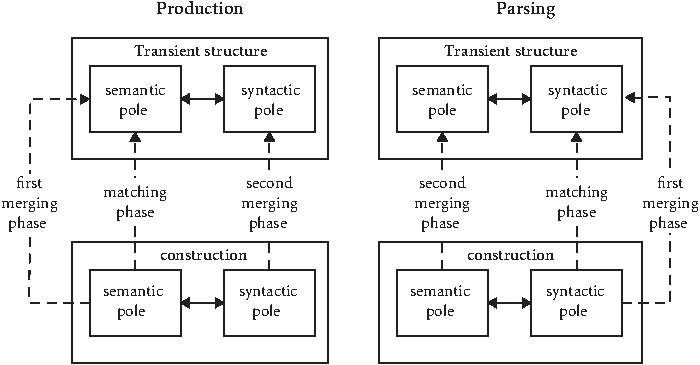
\includegraphics[width=.98\textwidth]{Figures/production-parsing-fcg.pdf}
\caption{\label{fig-matching-merging-trijp}FCG中的生成和句法分析\citep[\page 99]{vanTrijp2013a}}
%\caption{\label{fig-matching-merging-trijp}Generation and parsing in FCG \citep[\page 99]{vanTrijp2013a}}
\end{figure}%

\subsubsection{论元结构构式}
%\subsubsection{Argument Structure Constructions}

动变构式语法为论元结构假设了一个基于短语的处理方法,也就是说,假设词项进入一个能够提供独立意义的短语构造。\citep{vanTrijp2011a}。FCG方法是使用Goldberg插入方法分析论元结构构式的一个版本\citep{Goldberg95a}。Van Trijp认为每一个词项都能表征潜在的论元角色,如施事、受事、接受者和目标。短语论元结构构式与各自的词项结合并且实现部分论元角色,也就是说他们给这些论元角色一些语法功能。下一页中的图~\vref{fig-as-trijp}就展示了这样一个例子:动词sent(寄送)就有施事、受事、接受者和目标四个语义角色。基于被选择的论元结构构式,一些论元角色被选择实现。\footnote{%
这里值得注意的是, \citet[\page 141]{vanTrijp2011a}实际上提供了一个基于词汇的解释,因为每一个词项都通过同用(coapplication)连接来与不同短语构式连接。所以,每一个这样的词项和短语构式对都对应着词汇化树邻接语法(LTAG)中的一个词项。也参见 \citew[\page 25]{MWArgSt}对于Goldberg的假设的评论,假设是每一个词项都有短语构式关联。
注意这种同用关系是必要的,因为没有它们的话,这一方法就无法解释这样的例子,即两个或多个论元角色只能一起实现但是不能单独实现或者与另外列举出的角色组合。
}
%Fluid Construction Grammar assumes a phrasal approach to argument structure, that is, it is assumed that lexical items enter
%into phrasal configurations that contribute independent meaning \citep{vanTrijp2011a}. The FCG
%approach is one version of implementing Goldberg's plugging approach to argument structure
%constructions \citep{Goldberg95a}. Van Trijp suggests that every lexical item comes with a representation of
%potential argument roles like Agent, Patient, Recipient, and Goal. Phrasal argument structure
%constructions are combined with the respective lexical items and realize a subset of the argument
%roles, that is they assign them to grammatical functions. Figure~\vref{fig-as-trijp} shows an
%example: the verb \emph{sent} has the semantic roles Agent, Patient, Recipient, and Goal  (upper left
%of the figure). Depending
%on the argument structure construction that is chosen, a subset of these roles is selected for
%realization.\footnote{%
%  It is interesting to note here that  \citet[\page 141]{vanTrijp2011a} actually suggests a lexical
%  account since every lexical item is connected to various phrasal constructions via coapplication
%  links. So every such pair of a lexical item and a phrasal construction corresponds to a lexical
%  item in Lexicalized Tree Adjoining Grammar (LTAG). See also  \citew[\page 25]{MWArgSt} on
%  Goldberg's assumption that every lexical item is associated with phrasal constructions.

%Note that such coapplication links are needed since without them the approach cannot account for
%cases in which two or more argument roles can only be realized together but not in isolation or in
%any other combination with other listed roles.
%}
%\todostefan{Are there Agent Goal verbs or Patient Recipient or Patient Goal verbs that allow for
%  patterns that are impossible for sent?}
这一表格展示了寄送者、寄送物、接受者之间的关系以及更加抽象的语义角色之间的关系,还有这些角色与 (\mex{1})中语法功能的关系:
%The figures show the relation between sender, sent, and sendee and more the more abstract semantic
%roles and the relation between these roles and grammatical functions for the sentences in (\mex{1}):
\eal
\ex 
\gll He sent her the letter.\\
     他 寄送 她 \textsc{det} 信\\
\mytrans{他寄给她信。}
%He sent her the letter.
\ex 
\gll He sent the letter.\\
     他 寄送 \textsc{det} 信\\
\mytrans{他寄信。}
%He sent the letter.
\ex 
\gll The letter was sent to her.\\
      \textsc{det} 信 \passivepst{} 寄送 \textsc{prep} 她\\
\mytrans{这封信被寄送给她了。}
%The letter was sent to her.
\zl
虽然在 (\mex{0}a) 中,施事、受事和接受者都映射到语法功能上,但是在(\mex{0}b)中只有施事和受事映射到语法功能上。接受者被省略了。 (\mex{0}c)展示了一种论元实现,其中接受者实现为to短语。按照van Trijp的观点,这一语义角色不是一个接受者而是一个目标。
%While in (\mex{0}a) the agent, the patient and the recipient are mapped to grammatical functions,
%only the agent and the patient are mapped to grammatical functions in (\mex{0}b). The recipient is
%left out. (\mex{0}c) shows an argument realization in which the sendee is realized as a \emph{to}
%  phrase. According to van Trijp this semantic role is not a recipient but a goal. 

\begin{figure}
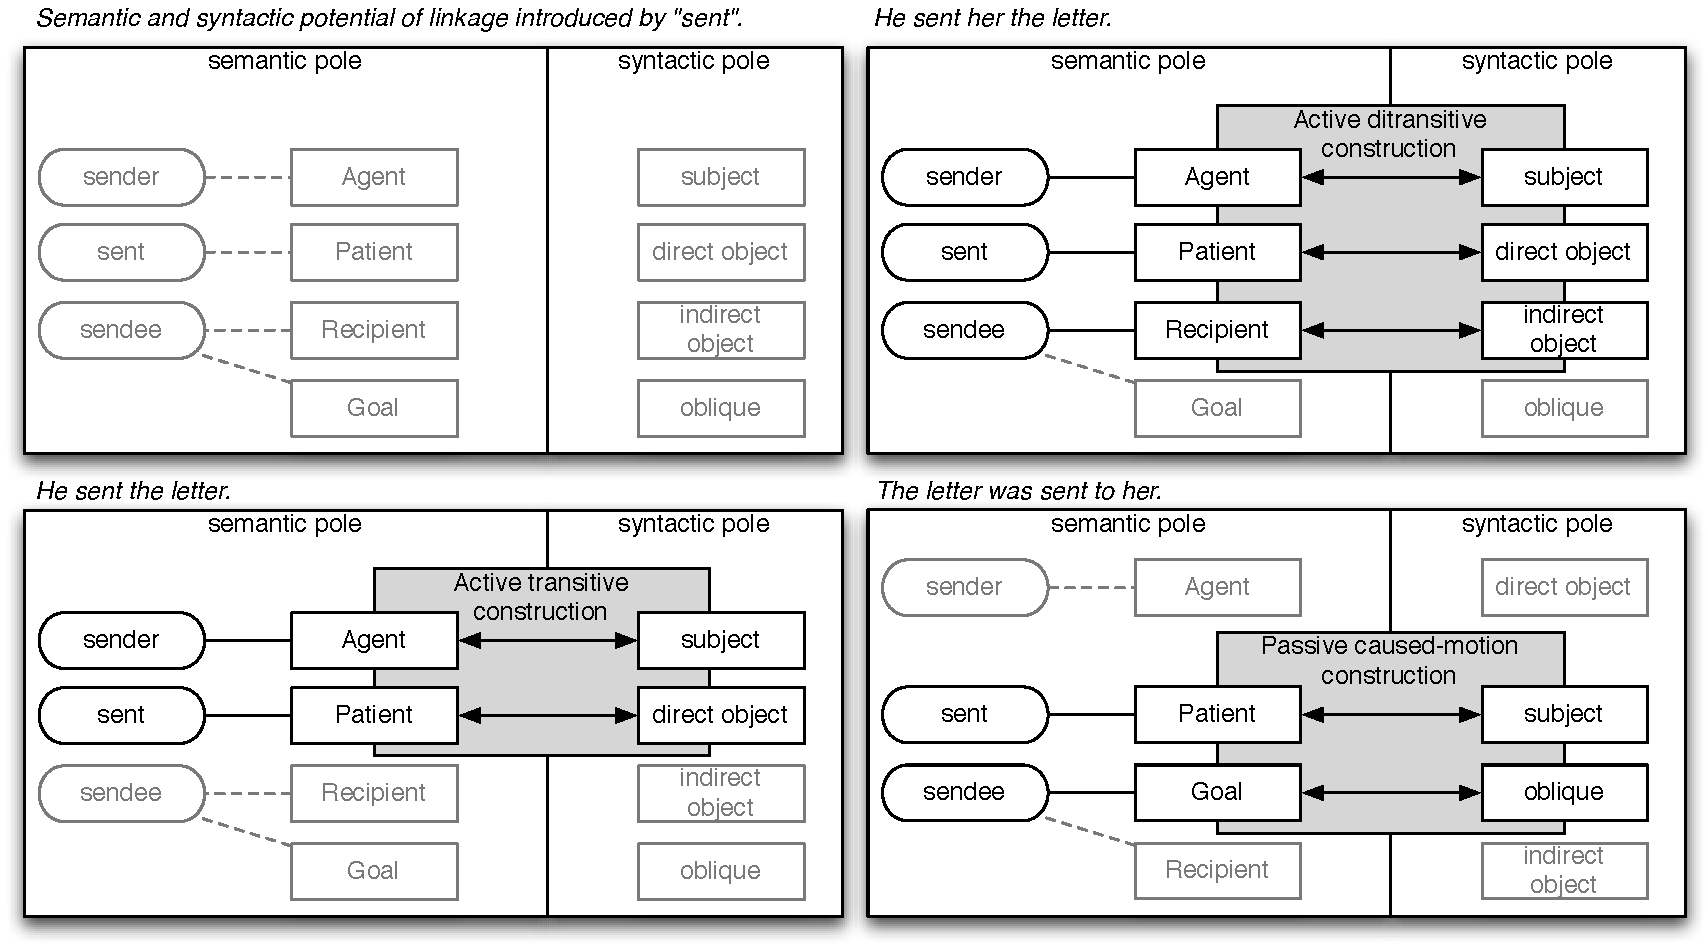
\includegraphics[width=\textwidth]{Figures/2011-van-Trijp.pdf}
\caption{\label{fig-as-trijp}词项和短语构式。图摘自 \citew[\page 122]{vanTrijp2011a}}
%\caption{\label{fig-as-trijp}Lexical items and phrasal constructions. Figure %taken 
%from  \citew[\page 122]{vanTrijp2011a}}
\end{figure}%

注意如果采用这一方法,就需要每一个主动构式都有一个被动变体。对于那些允许被动构式和无人称构式组合的语言来说,必须假设一个及物-被动-无人称构式。正如 \citew[\S~2.6]{Mueller2006d}所说,德语中的自由与格(commodi/incommodi)可以加到几乎所有构式上去。它们与与格被动构式互动,所以应该被当做论元。所以,对于动结构式,我们需要一个主动变体,一个被动变体,一个有与格论元的变体,一个有与格论元和与格被动的变体,一个中动变体。虽然,在技术上我们可以列举出所有这些模式,也可以想象我们可以把所有这些信息储存在我们脑子里,问题是这些列举是否真的反映了我们的语言学知识。如果一个新的构式产生了,我们就谈谈德语中带有一个主格两个与格的主动句模式吧,那么该句子模式有被动形式吗?虽然在主动和被动构式之间建立联系的观点会预测该句子模式会有被动形式,但是实际上没有这种可能。
%Note that under such an approach, it is necessary to have a passive variant of every active
%construction. For languages that allow for the combination of passive and impersonal constructions,
%one would be forced to assume a transitive-passive-impersonal construction. As was argued in
% \citew[Section~2.6]{Mueller2006d} free datives (commodi/incommodi) in German can be added to almost
%any construction. They interact with the dative passive and hence should be treated as
%arguments. So, for the resultative construction one would need an active variant, a passive variant,
%a variant with dative argument, a variant with dative argument and dative passive, and a middle variant.
%While it is technically possible to list all these patterns and it is imaginable that we store all
%this information in our brains, the question is whether such listings really reflect our linguistic
%knowledge. If a new construction comes into existence, lets say an active sentence pattern with a
%nominative and two datives in German, wouldn't we expect that this pattern can be used in the
%passive? While proposals that establish relations between active and passive constructions would
%predict this, alternative proposals that just list the attested possibilities do not.

怎样获得这种概括应该与HPSG中词库的组织联系起来讨论\citep{Flickinger87,Meurers2001a}。在词库中,可以按照词的价对所有动词进行分类并且说loves是一个及物动词,而被动变体loved是一个不及物动词。很明显这种方式忽略了loved和given有相同之处:它们都与其主动形式以一种系统的方式发生联系。与垂直概括相比,这种概括叫做水平概括,垂直概括描述承继层级中的上位类型和下位类型之间的关系。
%The issue of how such generalizations should be captured was discussed in connection with the
%organization of the lexicon in HPSG \citep{Flickinger87,Meurers2001a}. In the lexical world, one could simply categorize all verbs according to their
%valence and say that \emph{loves} is a transitive verb and the passive variant \emph{loved} is an
%intransitive verb. Similarly \emph{gives} would be categorized as a ditransitive verb and
%\emph{given} as a strictly transitive one. Obviously this misses the point that \emph{loved} and \emph{given}
%share something: they both are related to their active form in a systematic way. This kind of
%generalization is captured by lexical rules that relate two lexical items. The respective
%generalizations that are captured by lexical rules are called a horizontal generalizations as compared to vertical generalizations, which
%describe relations between subtypes and supertypes in an inheritance hierarchy.

这种概括是独立于词汇知识组织的,它也可以应用于短语表征。短语构式可以在层级(垂直)中组织,但是一些变体之间的关系不能用这种方式概括。与基于词汇方法中词汇规则相对应的是基于短语方法中类似于GPSG的元规则。所以,FCG中好像丢失的是连接短语模式的动词,例如同-构式(allo-constructions)(\citealp{Cappelle2006a};\citealp[\page  116]{Goldberg2014a},也可以参见脚注~\ref{fn-allostructions})。
%The issue is independent of the lexical organization of knowledge, it can be applied to phrasal
%representations as well. Phrasal constructions can be organized in hierarchies (vertical), but the
%relation between certain variants is not covered by this. The analog to the lexical rules in a
%lexical approach are GPSG-like metarules in a phrasal approach. So what seems to be missing in FCG
%is something that relates phrasal patterns, \eg allo"=constructions (\citealp{Cappelle2006a}; \citealp[\page
%  116]{Goldberg2014a}, see also footnote~\ref{fn-allostructions}).

\subsubsection{溶合、匹配和合并}
% \subsubsection{Fusion, matching and merging}

正如 \citet[\page 89--90]{Dowty89b-u}所指出的那样,在判断一个动词是否可以进入(或与之溶合)一个特定构式中时,仅仅核查语义兼容性是不够的。我们可以举出dine、eat和devour之间存在对立的例子。虽然吃的东西不一定与dine共现,但是可以与eat共现,并且一定要与devour共现。所以,词项一定要包含这些信息。
%As was pointed out by  \citet[\page 89--90]{Dowty89b-u}, checking for semantic compatibility is not sufficient
%when deciding whether a verb may enter (or be fused with) a certain construction. The example is
%the contrast between \emph{dine}, \emph{eat}, and \emph{devour}. While the thing that is eaten may
%not be realized with \emph{dine}, its realization is optional with \emph{eat} and obligatory with
%\emph{devour}. So the lexical items have to come with some information about
%this. 

\Citet{vanTrijp2011a}和 \citet{SvT2011a} 提出一个非常有趣的观点可以提供帮助:每一个动词都有一个潜在语义角色的列表,论元构式选择这些论元角色的字集(见图~\ref{fig-as-trijp})。这叫做匹配:不允许引入新的论元角色。这可以用来解释dine:我们可以说吃了某物,但是不存在题元角色可以与语法功能相连接。为了解释\isc{构式!致使-移动}\is{construction!Caused"=Motion}构式中出现的论元角色的扩展 \citep[\S~7]{Goldberg95a}, \citet{SvT2011a} 提出了一个叫“合并”的过程。合并被看做是一个修正策略:如果一个话段涉及一个不及物动词和一些别的材料,这一话段只用匹配原则就不能处理。例如,当处理(\mex{1})中Goldberg举出的例子的时候,he sneezed可以分析,但是foam和off the cappuccino则无法结合。(见第~\ref{chap-phrasal}章对这一构式的进一步讨论)。
%\Citet{vanTrijp2011a} and  \citet{SvT2011a} make an interesting suggestion that could help
%here: every verb comes with a list of potential roles and argument structure constructions can pick
%subsets of these roles (see Figure~\ref{fig-as-trijp}). This is called \emph{matching}: introducing new argument roles is not allowed. 
%This would make it possible to account for \emph{dine}: one could
%say that there is something that is eaten, but that no Theme role is made available for linking to
%the grammatical functions. This would be a misuse of thematic roles for syntactic purposes though
%since \emph{dine} is semantically a two-place predicate. To account for the extension of argument roles as it is observed in the
%Caused"=Motion Construction\is{construction!Caused"=Motion} \citep[Chapter~7]{Goldberg95a},  \citet{SvT2011a} suggest a process called \emph{merging}. Merging is seen
%as a repair strategy: if an utterance involves an intransitive verb and some other material, the
%utterance cannot be processed with matching alone. For example, when processing Goldberg's example
%in (\mex{1}), \emph{he sneezed} could be parsed, but \emph{the foam} and \emph{off the cappuccino}
%would be unintegrated (see Chapter~\ref{chap-phrasal} for an extended discussion of such constructions).
\ea
\gll He sneezed the foam off the cappuccino.\\
     他 打喷嚏 \textsc{det} 泡沫 \textsc{prep} \textsc{det}  卡布奇诺咖啡\\
\mytrans{他打喷嚏把泡沫从卡布奇诺咖啡上吹走了。}
%He sneezed the foam off the cappuccino.
\footnote{%
 \citew[\page 42]{Goldberg2006a}。
}
\z
所以, \citet[\page 319--320]{SvT2011a}表明只有当常规构式不能应用的时候,才允许合并。这一方法的问题在于人类语言是高度歧义的并且在这种情况下这会导致一种状况,在这种状况中一个话段有一个意思,所以这一修复策略不会有效。考虑(\mex{1}):\footnote{%
  我为这些例子感到抱歉……
}
%So,  \citet[\page 319--320]{SvT2011a} suggest that only if regular constructions cannot apply, merging is
%allowed. The problem with this is that human language is highly ambiguous and in the case
%at hand this could result in situations in which there is a reading for an utterance, so that the
%repair strategy would never kick in. Consider (\mex{1}):\footnote{%
%  I apologize for these examples \ldots
%}
\ea
\label{ex-schlag-den-mann-tot}
\gll Schlag den Mann tot!\\
     击打   \textsc{det} 男人  死\\
\mytrans{把这个男人打死!' 或者 `打这个死人!}
%\gll Schlag den Mann tot!\\
%     beat   the man  dead\\
%\mytrans{Beat the man to death!' or `Beat the dead man!}
\z
(\mex{0}) 有两个意义:结果义,其中tot(死)表示打的结果;在另外一个意义中,tot是一个描述性谓词。第二种解释是不常见的,因为打已经死去的人这一活动是不常见的,但是这一结构与带有描述性谓词的句子是平行的。
%(\mex{0}) has two readings: the resultative reading in which \emph{tot} `dead' expresses the result of the
%beating and another reading in which \emph{tot} is a depictive predicate. The second reading is
%dispreferred, since the activity of beating dead people is uncommon, but the structure is parallel to
%other sentences with depictive predicates:
\ea
\gll Iss den Fisch roh!\\
     吃 \textsc{det} 鱼 生的\\
%\gll Iss den Fisch roh!\\
%     eat the fish raw\\
\z
可以让tot与一个不能理解为结果谓词的谓词并列来强制将tot理解为描述义:
%The depictive reading can be forced by coordinating \emph{tot} with a predicate that is not a
%plausible result predicate:
\ea
\gll Schlag ihn tot oder lebendig!\\
     击打   他 死 或者 活着\\
\mytrans{在他死之后或者还活着的时候打他!}
%\gll Schlag ihn tot oder lebendig!\\
%     beat   him dead or alive\\
%\mytrans{Beat him when he is dead or while he is alive!}
\z
所以,问题是(\ref{ex-schlag-den-mann-tot}) 含有一个意义不需要激活修复机制:schlug(击打)应用于一个及物构式而tot是一个附加语(参看\citealp{Winkler97a})。但是, (\ref{ex-schlag-den-mann-tot}) 更加可能的一个分析是结果分析,在这种分析中价框架通过一个旁格元素得到扩展。所以,这意味着我们必须允许合并操作独立于其他可能的操作。正如 \citet[\page 320]{SvT2011a}指出的那样,如果合并不能自由使用,像(\mex{1}a)这种话段就不被允许,当然(\mex{1}b) 也是这样。
%So, the problem is that (\ref{ex-schlag-den-mann-tot}) has a reading which does not require the invocation of the repair mechanism: \emph{schlug} `beat' is used with the transitive
%construction and \emph{tot} is an adjunct (see \citealp{Winkler97a}). However, the more likely analysis of (\ref{ex-schlag-den-mann-tot}) is the one
%with the resultative analysis, in which the valence frame is extended by an oblique element. So this
%means that one has to allow the application of merging independent of other analyses that might be possible.
%As  \citet[\page 320]{SvT2011a} note, if merging is allowed to apply freely, utterances like
%(\mex{1}a) will be allowed and of course (\mex{1}b) as well.
\eal
\ex[*]{
\gll She sneezed her boyfriend.\\  
    她 打喷嚏 她的 男朋友\\
%She sneezed her boyfriend.
}
\ex[*]{
\gll She dined a steak.\\  
    她 吃饭 一 牛排\\
%She dined a steak.
}
\zl
在(\mex{0}) 中,sneeze和dine都用于及物构式当中。
%In (\mex{0}) \emph{sneeze} and \emph{dined} are used in the transitive construction.

摆脱这一困境的方法是在词项中建立描述动词使用句法环境的信息。这种信息可以进行加权,例如dine用作及物动词的概率很低。Steels和van Trijp可能会通过所谓共用连接(coapplication)来联系词项与短语构式,并且dine和及物构式之间的连接强度会很低,sneeze和致使移动\isc{构式!致使-移动}\is{construction!Caused"=Motion}构式之间的连接强度会很高。这会解释这一现象(并且采用基于使用的方式),但是在CG、HPSG、SBCG和DG中将会使用一种词汇方法。
%The way out of this dilemma is to establish information in lexical items that specifies in which
%syntactic environments a verb can be used. This information can be weighted and for instance the
%probability of \emph{dine} to be used transitively would be extremely low. Steels and van Trijp
%would connect their lexical items to phrasal constructions via so-called coapplication links and the
%strength of the respective link would be very low for \emph{dine} and the transitive construction and
%reasonably high for \emph{sneeze} and the Caused"=Motion Construction\is{construction!Caused"=Motion}. This would explain the
%phenomena (and in a usage"=based way), but it would be a lexical approach, as it is common in CG, HPSG,
%SBCG, and DG.

\subsubsection{长距离依存}
%\subsubsection{Long-distance dependencies}
\label{sec-fcg-nld}

\Citet{vanTrijp2014a} 对比了GPSG、HPSG、SBCG中运用的基于\slaschc 的方法和他在FCG框架中使用的方法。他认为SBCG与FCG有根本上的差别,并且将SBCG归入生成语法的范畴,将FCG归入认知功能语法的范畴。他表明他的认知功能方法在完整性质、解释充分性和理论简约性上更有优势(第2页)。 \citet{vanTrijp2014a}说明的基本上是 \citet{Reape2000a}在一个未发表的的文章中的一个分析。(见 \citew{Reape94a}一个发表的版本对基于线性化方法的论述以及 \citew{Kathol2000a,Babel,Mueller99a,Mueller2002b}基于线性化的方法,这一方法虽然是基于线性化的,但是仍然为非局部依存假设了\slaschc 方法)。Van Trijp发展了一个语法模型,允许不连续成分并且只是将(\mex{1})所示句子中宾语的序列化看作另外的线性化选择。
%\Citet{vanTrijp2014a} compares the \slasch-based approaches that are used in GPSG, HPSG, and SBCG
%with the approach that he suggests within the framework of FCG. He claims that there are fundamental
%differences between SBCG and FCG and assigns SBCG to the class of generative grammars, while
%placing FCG in the class of cognitive"=functional approaches. He claims that his
%cognitive"=functional approach is superior in terms of completeness, explanatory adequacy, and
%theoretical parsimony (p.\,2). What  \citet{vanTrijp2014a} suggests is basically an analysis that was
%suggested by  \citet{Reape2000a} in unpublished work (see  \citew{Reape94a} for a published version of
%an linearization"=based approach and  \citew{Kathol2000a,Babel,Mueller99a,Mueller2002b} for
%linearization"=based approaches that despite of being linearization"=based assume the \slasch approach for nonlocal dependencies). Van Trijp
%develops a model of grammar that allows for discontinuous constituents and just treats the
%serialization of the object in sentences like (\mex{1}) as an alternative linearization option.
\eal
\ex 
\gll This book, I read.\\  
    这 书 我 读\\
\mytrans{这本书,我读。}
%This book, I read.
\ex 
\gll What did the boy hit?\\  
    什么 \textsc{aux} \textsc{det} 男孩 击打\\
\mytrans{这个男孩击打了什么?}
%What did the boy hit?
\zl
Van Trijp的分析涉及到几种一般不会出现在短语结构语法中的单位,但是可以通过邻接限制来刻画或者表征要素之间的关系,这些关系在HPSG/SBCG中是词汇表征的一部分。一个例子是主语-动词锚位,这一锚位连接了主语和动词来表征这两个元素扮演重要的语法角色。图~\vref{fig-what-did-the-boy-hit}展示了对 (\mex{1})的分析。
%Van Trijp's analysis involves several units that do not normally exist in phrase structure grammars,
%but can be modeled via adjacency constraints or represent relations between items which are part
%of lexical representations in HPSG/SBCG anyway. An example is the subject-verb anchor that connects
%the subject and the verb to represent the fact that these two items play an important functional
%role. Figure~\vref{fig-what-did-the-boy-hit} shows the analysis of (\mex{1}).
\ea
\gll What did the boy hit?\\  
    什么 \textsc{aux} \textsc{det} 男孩 击打\\
\mytrans{这个男孩在击打什么?}
%What did the boy hit?
\z
\begin{figure}
\begin{forest}
for tree={l sep+=5mm}
%l sep+=10mm
[TRANSITVE-CLAUSE-UNIT, name=tcu
  [NP-UNIT-1, name=np1
    [PRO [what\\什么]] ]
  [\textsc{aux},tier=det, no edge, name=aux [did\\\textsc{aux}] ]
  [NP-UNIT-2, name=np2
    [\textsc{det}, tier=det [the\\\textsc{det}]]
    [N   [boy\\男孩]] ]
  [VP-UNIT, name=vp
    [V [hit\\击打] ] ]
]
\draw (vp.south)--(aux.north);
\node (topic) [base left=of tcu]
    {
        TOPIC-UNIT
    };
\draw[dashed] (topic.south)--(np1.north);
\node (focus) [below=0mm of tcu.south west]
    {
        FOCUS-UNIT
    };
\draw[dashed] (focus.south)--(np1.north);
\draw[dashed] (focus.south)--(aux.north);
\node (sau) [base right= of tcu]
    {
        SV-ANCHOR-UNIT
    };
\draw[dashed] (sau.south)--(vp.north);
\draw[dashed] (sau.south)--(np2.north);
\end{forest}
\caption{\label{fig-what-did-the-boy-hit}根据 \citet[\page 265]{vanTrijp2014a}的对What did the boy hit?的分析}
%\caption{\label{fig-what-did-the-boy-hit}The analysis of \emph{What did the boy hit?} according to
%   \citet[\page 265]{vanTrijp2014a}}
\end{figure}%
正如上表所示,van Trijp也借助了信息结构的术语,例如话题和焦点。这里需要注意的一点是,对于信息结构l\isc{信息结构} l\is{information structure}的分析在HPSG框架中有很长的历史\citep{EV96a, Kuhn95b,Kuhn96a,
GuntherMaienborn1999,Wilcock2001a,deKuthy2002a,Paggio2005a-u,Bildhauer2008a,BC2010a}。在  \citew{Sag2012a}等人探讨句法的论文中没有涉及信息结构并不意味着HPSG/SBCG理论忽略了信息结构或者认为信息结构应该被忽略。对于完整性来说这很重要。这一点对于解释充分性当然也是一样。这给予了理论简约性,但是在我们评论之前,我想先具体讨论一下van Trijp的分析以便于能显示他的很多观点在实践上都是有问题的,并且因此他的理论不具有解释力,因为实践上的正确性是解释充分性的前提。
%As can be seen in the figure, van Trijp also refers to information structural\is{information structure} terms
%like topic and focus. It should be noted here that the analysis of information structure has quite
%some history in the framework of HPSG  \citep{EV96a, 
%Kuhn95b,Kuhn96a, 
%GuntherMaienborn1999,
%Wilcock2001a, 
%deKuthy2002a,Paggio2005a-u, 
% \citet{Webelhuth2007a-u}, 
%Bildhauer2008a,BC2010a}. The fact that information structure is not talked about in syntax
%papers like  \citew{Sag2012a} does not entail that information structure is ignored or should be
%ignored in theories like HPSG and SBCG. So much for completeness. The same holds of course for
%explanatory adequacy. This leaves us with theoretical parsimony, but before I comment on this, I
%want to discuss van Trijp's analysis in a little bit more detail in order to show that many of his claims
%are empirically problematic and that his theory therefore cannot be explanatory since empirical
%correctness is a precondition for explanatory adequacy.
Van Trijp表示英语中包含非局部依存构式的句子以话题开头\footnote{%
\Citet[\page 256]{vanTrijp2014a}采用的话题和焦点的定义如下:“话题性(topicality)是从相关性的角度进行定义的:一个话段的话题就是这个话段相关的部分”。焦点性(focality)是从重要性的角度进行定义的并且是为凸显在当前交际语境中最重要的信息。
}。Bresnan举出的例句(\ref{bsp-fronted-focus})、(\ref{bsp-fronted-topic}) 在第~\pageref{bsp-fronted-focus}页\citep[\page 97]{Bresnan2001a}已经讨论过了,为了方便这里重复如下:
%Van Trijp claims that sentences with nonlocal dependency constructions in English start with a
%topic.\footnote{%
%\Citet[\page 256]{vanTrijp2014a} uses the following definitions for topic and focus: ``Topicality is defined in terms of aboutness: the topic of an utterance
%is what the utterance is `about'. Focality is defined in terms of salience:
%focus is used for highlighting the most important information given the
%current communicative setting.''
%} Bresnan's sentences in (\ref{bsp-fronted-focus}) and (\ref{bsp-fronted-topic}) were discussed on page~\pageref{bsp-fronted-focus}
%\citep[\page 97]{Bresnan2001a} and are repeated below for convenience:
\ea
\label{bsp-fronted-focus-two}
\gll Q: What did you name your cat?\\  
     问: 什么 \textsc{aux} 你 命名 你的 猫\\
\mytrans{你给你的猫取什么名?}

\gll A: Rosie I named her. \\
     答: Rosie 我 命名 她\\\jambox{(\emph{Rosie} = \textsc{focus})}
\mytrans{我叫她Rosie。}
%Q: What did you name your cat?\\
%A: Rosie I named her. (\emph{Rosie} = \textsc{focus})
\z
\ea
\label{bsp-fronted-topic-two}
\gll Q: What did you name your pets?\\    
     问: 什么 \textsc{aux} 你 命名 你的 宠物\\
\mytrans{你叫你的宠物什么名字?} 

\gll A: My dog, I named Harold. My cat, I named Rosie.\\
     答: 我的 狗 我 命名 Harold 我的 猫 我 命名 Rosie\\\jambox{(\emph{my dog}, \emph{my cat} = \textsc{topic})}
\mytrans{我的狗,我叫他Harold。我的猫,我叫她Rosie。}
%Q: What did you name your pets?\\
%A: My dog, I named Harold. My cat, I named Rosie. (\emph{my dog}, \emph{my cat} = \textsc{topic})
\z
这些句子表明主语之前的位置既可能是话题也可能是焦点。所以,前置的成分就是话题这一说法在实践上是不对的。如果这一位置与信息结构功能联系起来的话,这一联系应该是一个析取式,允许话题成分和焦点成分。
%These sentences show that the pre-subject position is not unambiguously a topic or a focus
%position. So, a statement saying that the fronted element is a topic is empirically not correct. If this position is to be associated with an information structural function, this
%association has to be a disjunction admitting both topics and focused constituents.

Van Trijp分析的另外一个问题是,他假设助动词do是一个宾语标记(第10、22页) 或者是一个非主语标记(第23页)。(\mex{1}a)中的主语问句确实不需要do支撑,只有 (\mex{1}b)中的问句需要,但是这并不意味着do之后的所有元素都是宾语。
%A further problematic aspect of van Trijp's analysis is that he assumes that the auxiliary \emph{do}
%is an object marker (p.\,10, 22) or a non-subject marker (p.\,23). It is true that \emph{do} support is not necessary in subject questions like
%(\mex{1}a), but only in (\mex{1}b), but this does not imply that all items that are followed by
%\emph{do} are objects.
\eal
\ex 
\gll Who saw the man?\\  
     谁 看见 \textsc{det} 男人\\
\mytrans{谁看见了这个男人?}
%Who saw the man?
\ex 
\gll Who did John see?\\  
     谁 \textsc{aux} John 看见\\
\mytrans{John看见了谁?}
%Who did John see?
\zl
首先,do可以用于强调动词:
%First, \emph{do} can be used to emphasize the verb:
\ea
\gll Who \emph{did} see the man?\\  
     谁 \textsc{aux} 看见 \textsc{det} 男人\\
\mytrans{谁看见了这个男人?}
%Who \emph{did} see the man?
\z
其次,所有类型的其他语法词都可以出现在动词之前:
%Second, all types of other grammatical functions can precede the verb:
\eal
\settowidth\jamwidth{(prepositional object)}
\ex
\gll Where did you see the man?\\    
     哪里 \textsc{aux} 你 看见 \textsc{det} 男人\\\jambox{(adverbial)}
\mytrans{你在哪里看见了这个男人?}
%Where did you see the man? \jambox{(adverbial)}
\ex 
\gll How tall is the man?\\     
     怎样 高 \textsc{cop} \textsc{det} 男人\\\jambox{(predicative)}
\mytrans{这个男人有多高?}
%How tall is the man? \jambox{(predicative)}
\ex
\gll What did John consider Peter?\\     
     什么 \textsc{aux} John 认为 Peter\\ \jambox{(predicative)}
\mytrans{John认为Peter是什么?}
%What did John consider Peter? \jambox{(predicative)}
\ex 
\gll What does this book cost?\\
     什么 \textsc{aux} 这 书 花费\\       \jambox{(adverbial)}
\mytrans{这本书花费了多少钱?}
%What does this book cost? \jambox{(adverbial)}
\ex 
\gll About what did you talk?\\       
     关于 什么 \textsc{aux} 你 说\\ \jambox{(prepositional object)}
\mytrans{你谈论了什么?}
%About what did you talk? \jambox{(prepositional object)}
\zl
最后,即便是主语也可以出现在do之前,只要这个主语是从其他小句提取出来的。
%And finally, even a subject can appear in front of \emph{do} if it is extracted from another clause:
\ea
\settowidth\jamwidth{(prepositional object)}
\gll Who does he think saw this man?\\   
     谁 \textsc{aux} 他 认为 看见 这 男人\\\jambox{(subject)}
\mytrans{他认为谁看见了这个男人?}
%Who does he think saw this man? \jambox{(subject)}
\z
%
% Auch die linke Peripherie kann man ja einfach als kontinuierlich einordnen. Brauche Beleg für
% Extraposition aus pränominalem Adjunkt. Das würde mögliche Diskontinuität zeigen.
%
%% Van Trijp does not address the issue of island constraints. Extraction islands are areas that nobody
%% can leave, that is, extraction is excluded. For instance, it is impossible to extract from the
%% prenominal area in English and German (Ross' Left Branch Condition).
%\ea
%der die Frau liebende Mann, die ... erfunden hat
%%  and it is also impossible to
%% extract out of a relative clause:
%% % Er könnte sagen, dass Relativsätze immer kontinuierlich sein müssen.
%% \ea
%% This man$_i$, I saw a women [who likes \_$_i$ ].
%% \z
%% \slasch"=based models assume that relative clauses involve internal nonlocal dependencies, but no
%% \slasch dependency leaves the relative clause. This is ensured by the schemata that combine the
%% relative pronoun and the remaining clause.

还有另外一个实践性问题:假设填充语与其来源存在联系的方法可以解决辖域歧义问题,这种辖域歧义只有当某一元素提取才会产生。例如,对比 (\mex{1}a) 中的句子与 (\mex{1}b, c)中的句子:虽然在 (\mex{1}a) 、(\mex{1}c)中oft(经常)与nicht(不)的顺序是一样的,(\mex{1}a) 存在歧义但是 (\mex{1}c) 不存在。
%There is a further empirical problem: approaches that assume that a filler is related to its origin
%can explain s\textsc{cop}e ambiguities that only arise when an element is extracted. Compare for instance the
%sentence in (\mex{1}a) with the sentences in (\mex{1}b, c): although the order of \emph{oft} `often' and
%\emph{nicht} `not' in (\mex{1}a) and (\mex{1}c) is the same, (\mex{1}a) is ambiguous but (\mex{1}c) is
%not.
\eal
\ex 
\gll Oft liest er das Buch nicht.\\
     经常 读 他 \textsc{det} 书 不\\
\mytrans{大多数情况下他不读这本书。' 或者 `他并非经常读这本书。}
%\gll Oft liest er das Buch nicht.\\
%     often reads he the book not\\
%\mytrans{It is often that he does not read the book.} or `It is not the case that he reads the book
%often.'
\ex
\gll dass er das Buch nicht oft liest\\
     \textsc{comp} 他 \textsc{det} 书 不 经常 读\\
\mytrans{他并非经常读这本书这件事}
%\gll dass er das Buch nicht oft liest\\
%     that he the book not often reads\\
%\mytrans{that it is not the case that he reads the book often}
\ex
\gll dass er das Buch oft nicht liest\\
     \textsc{comp} 他 \textsc{det} 书 经常 不 读\\
\mytrans{大多数情况下他并不读这本书这件事}
%\gll dass er das Buch oft nicht liest\\
%     that he the book often not reads\\
%\mytrans{that it is often that he does not read the book}
\zl
(\mex{0}a)有两个意义分别对应于(\mex{0}b) 和 (\mex{0}c)。一个纯粹基于线性化的方法难以解释这一问题。一个基于\slaschc 的方法可以假设 (\mex{0}a) 在oft位置(在 (\mex{0}b) 或者 (\mex{0}c))有一个缺位(或者一些类似的引入非局部依存的方法)。在意义组合过程中,缺位的信息应该将缺位的位置考虑在内。这就自动解释了观察到的意义。
%(\mex{0}a) has the two readings that correspond to (\mex{0}b) and (\mex{0}c). A purely
%linearization"=based approach probably has difficulties to explain this. A \slasch"=based approach
%can assume that (\mex{0}a) has a gap (or some similar means for the introduction of nonlocal
%dependencies) at the position of \emph{oft} in (\mex{0}b) or (\mex{0}c). The gap information is
%taken into account in the semantic composition at the site of the gap. This automatically accounts
%for the observed readings.

另外一个不得不解释的现实问题是存在标记提取路径\isc{提取路径标记}\is{extraction path marking}的语言。 \citet*{BMS2001a}列出了大量语言,在这些语言里元素会因其所依附的成分是否有缺位而不同。例如,爱尔兰语有一种标补语,当其所依附小句含有被提取元素时是一种形式,当其所依附小句不含被提取元素时是另外一种形式。基于\slaschc 的方案可以直接解释这种现象:一个短语中缺少一个成分是在语迹的\slaschc 取值中表征并且这种信息可以上滤到树上去。所以即使复杂结构也包含它们当中丢失了一个成分这一信息。与句子组合的标补语因此可以选择带有与其屈折对应\slaschc 取值的句子。Van Trijp对于这一挑战的回答是所有的语言都是不同的\citep[\page 263]{vanTrijp2014a}并且源于一个语言的证据并不一定意味着对那一语言的分析也对另外一种语言适用。虽然我原则上同意这一观点(参看\ref{sec-syntactic-universals}),但是我认为提取是语言的一种根本属性并且对于具有非局部依存的语言来说,非局部依存应该用相同的方式分析。
%Another empirical problem that has to be solved is the existence of extraction path
%marking\is{extraction path marking}
%languages.  \citet*{BMS2001a} list a number of languages in which elements vary depending on the
%existence or absence of a gap in a constituent they attach to. For instance, Irish has
%complementizers that have one form if the clause they attach to has an element extracted and another
%form if it does not. \slasch-based proposals can account for this in a straight-forward way: the
%fact that a constituent is missing in a phrase is represented in the \slashv of the trace and this
%information is percolated up the tree. So even complex structures contain the information that there
%is a constituent missing inside them. Complementizers that are combined with sentences therefore can
%select sentences with \slashvs that correspond to their inflection.
%Van Trijp's answer to this challenge is that all languages are different
%\citep[\page 263]{vanTrijp2014a} and that the evidence from one language does not necessarily mean that the analysis for that language is
%also appropriate for another language. While I agree with this view in principle (see
%Section~\ref{sec-syntactic-universals}), I do think that extraction is a rather fundamental property
%of languages and that nonlocal dependencies should be analyzed in parallel for those languages that
%have it.

\subsection{并列}
%\subsection{Coordination}
\label{sec-coordination}

非转换语法的一个成功案例是  \citet{Gazdar81}对于非局部依存的基于\slaschc 的分析。这一分析第一次解释了Ross提出的跨界抽取\isc{跨界抽取}\is{Across the Board Extraction}\citep{Ross67}。这些例子在第~\pageref{ex-atb-gazdar}页已经讨论过了,为了方便这里重复如下:
%One of the success stories of non-transformational grammar is the \slasch-based analysis of nonlocal dependencies
%by  \citet{Gazdar81}. This analysis made it possible for the first time to explain Ross's Across the Board
%Extraction\is{Across the Board Extraction} \citep{Ross67}. The examples were already discussed on
%page~\pageref{ex-atb-gazdar} and are repeated here for convenience:
\eal\settowidth\jamwidth{(= S/NP \& S/NP)}
\label{ex-atb-gazdar-two}
\ex[]{ %The kennel     which Mary made and Fido sleeps in has been stolen.	 \jambox{(= S/NP \& S/NP)}
\gll The kennel     which Mary made and Fido sleeps in has been stolen.\\   
    \textsc{det}  狗窝 \textsc{rel} Mary 做 并且 Fido 睡 \textsc{prep} \textsc{aux} \passive{} 偷\\\jambox{(= S/NP \& S/NP)}
\mytrans{Mary制作并且Fido在里面睡的那个狗窝被人偷走了。}
}
\ex[]{ %The kennel in which Mary keeps drugs and Fido sleeps has been stolen.	\jambox{(= S/PP \& S/PP)}
\gll The kennel in which Mary keeps drugs and Fido sleeps has been stolen.\\   
    \textsc{det}  狗窝 \textsc{prep} \textsc{rel} Mary 保持 药物 并且 Fido 睡 \textsc{aux} \passive{} 偷\\\jambox{(= S/PP \& S/PP)}
\mytrans{Mary放药物并且Fido在里面睡的那个狗窝被人偷走了。}
}
\ex[*]{%The kennel (in) which Mary made and Fido sleeps has been stolen.     \jambox{(= S/NP \& S/PP)}
\gll The kennel (in) which Mary made and Fido sleeps has been stolen.\\     
    \textsc{det}  狗窝 \hspaceThis{(}\textsc{prep} \textsc{rel} Mary 做 并且 Fido 睡 \textsc{aux} \passive{} 偷\\\jambox{(= S/NP \& S/PP)}
}
\zl
上面例子的共性是如果两个或多个成分有相同的句法范畴和相同的\slashvsc 取值的话,它们就可以并列。这就解释了(\mex{0}a、b)中的which和in which为什么可以在各自的小句中填充两个位置。那么,不采用\slashfc 来分析缺失成分信息弥散的理论就必须寻找另外的方式去确保所有的论元槽被填充并且被提取成分和相应的论元角色之间的关系是正确的。注意这一点在van Trijp提出的模型中并不直接,因为他必须允许介词in与它左边的一些成分组合,这些成分同时也是made的主语。通常一个NP不能简单地充当两个中心语的论元。见例(\mex{1}a):
%The generalization is that two (or more) constituents can be coordinated if they have identical
%syntactic categories and identical \slashvs. This explains why \emph{which} and \emph{in which} in
%(\mex{0}a,b) can fill two positions in the respective clauses. Now, theories that do not use a
%\slashf for the percolation of information about missing elements have to find different ways to
%make sure that all argument slots are filled and that the correct correspondence between extracted
%elements and the respective argument role is established. Note that this is not straightforward in
%models like the one suggested by van Trijp, since he has to allow the preposition \emph{in} to be
%combined with some material to the left of it that is simultaneously also the object of
%\emph{made}. Usually an NP cannot simply be used by two different heads as their argument. As an
%example consider (\mex{1}a):
\eal
\ex[*]{
\gll John said about the cheese that I like.\\
    John 说 \textsc{prep} \textsc{det} 奶酪 \textsc{comp} 我 喜欢\\
%John said about the cheese that I like.
}
\ex[]{
\gll John said about the cheese that I like it.\\
    John 说 \textsc{prep} \textsc{det} 奶酪 \textsc{comp} 我 喜欢 它\\
\mytrans{John谈论了我喜欢的那种奶酪。}
%John said about the cheese that I like it.
}
\zl
如果一个材料可以多次使用,那么 (\mex{0}a) 中的结构就是可能的,在这一结构中the cheese是介词about和动词like的宾语。但是,这个句子是完全不合法的:代词it必须要去填充宾语槽。
% (\mex{0}a) If it would be possible to use material several times, a structure for (\mex{0}a) would be possible
%in which \emph{the cheese} is the object of the preposition \emph{about} and of the verb
%\emph{like}. This sentence, however, is totally out: the pronoun \emph{it} has to be used to fill
%the object slot.

\subsection{不连续成分和语言使用模型}
%\subsection{Discontinuous constituents and performance models}

Van Trijp指出SBCG没有一个语言使用模型并且拿这一点与FCG进行对比。在第252页,他指出:

%Van Trijp points out that SBCG does not have a performance model and contrasts this with FCG. On
%page~252 he states:
\begin{quotation}
所以,句法分析始于将话段分解为不同的形式,这些形式通过形态和词汇构式范畴化为单词,这些单词结合成短语(可以参见Steels, 2011b,看一下FCG中词库-短语处理的更细致的解释)。所以句法分析器会为所有四个话段寻找相似的成分,正如例(21-24)所示。因为在例(24)中助动词do不在VP的直接域之内,所以没有被识别为VP的一个成员。

所有这些短语都是没有联系的,这意味着语法仍然需要说明这些短语之间的关系。\citep[\page 252]{vanTrijp2014a}\footnote{
So parsing starts by segmenting the utterance
into discrete forms, which are then categorized into words by morphological
and lexical constructions, and which can then be grouped together as
phrases (see Steels, 2011b, for a detailed account of lexico-phrasal
processing in FCG). So the parser will find similar constituents for all
four utterances, as shown in examples (21--24). Since auxiliary-\emph{do} in
example (24) falls outside the immediate domain of the VP, it is not yet
recognized as a member of the VP.

All of these phrases are disconnected, which means that the grammar
still has to identify the relations between the phrases. 
}
\end{quotation}
在 (21)--(24)中,van Trijp为主语和宾语提供了几个包含NP的树片段并且表明这些树片段必须组合在一起以便于分析他所讨论的句子。在实际处理中这是不够的:如果FCG没有区分语言能力/语言运用,那么话段分析的方式应该反映人类处理语言的方式(并且这也是FCG经常所标榜的)。但是,我们所知道的关于人类语言处理的一切都指向一个渐进式处理,也就是说,只要信息存在我们就处理它。我们开始处理第一个词语时考虑其所有相关方面(音系、重音、词类、语义和信息结构)并且提出关于话段应该如何处理的一种假设。只要我们处理了两个单词(实际上更早,在处理单词时整合已经发生)我们将第二个单词整合进我们已经知道的并且继续沿着我们的假设及逆行,或者修正它,或者失败。参看\ref{Abschnitt-Inkrementelle-Verarbeitung}获得处理的细节以及对于显示处理是渐进的实验的讨论。所以,我们说van Trijp的分析在实践层面上失败了:他对于语言使用层面的建模是不足的。
%In his (21)--(24), van Trijp provides several tree fragments that contain NPs for subject and object and states that
%these have to be combined in order to analyze the sentences he discusses. This is empirically
%inadequate: if FCG does not make the competence/performance distinction, then the way utterances are
%analyzed should reflect the way humans process language (and this is what is usually claimed about FCG). However, all we know about human language
%processing points towards an incremental processing, that is, we process information as soon as it
%is available. We start to process the first word taking into account all of the relevant aspects
%(phonology, stress, part of speech, semantics, information structure) and come up with an hypothesis
%about how the utterance could proceed. As soon as we have two
%words processed (in fact even earlier: integration already happens during the processing of words) we integrate the second word
%into what we know already and continue to follow our hypothesis, or revise it, or simply fail. See
%Section~\ref{Abschnitt-Inkrementelle-Verarbeitung} for details on processing and the discussion of
%experiments that show that processing is incremental. So, we have to say that van Trijp's analysis
%fails on empirical grounds: his modeling of performance aspects is not adequate.

Van Trijp所描述的分析方案与HPSG分析器十分相似,但是这些方案通常没有关于人类语言运用的任何说明。对语言运用进行建模十分复杂,因为很多因素都起作用。所以,合理的做法应该是像HPSG和FCG那样将语言运用和语言能力分开。这并不意味着语言运用方面不去建模,实际上运用HPSG的心理语言学模型过去曾经有人开发过\citep{Konieczny96a-u},但是发展出一个有很大覆盖性的语法以及与它组合的语言运用模型需要大量资源。
%The parsing scheme that van Trijp describes is pretty much similar to those of computational HPSG parsers, but
%these usually come without any claims about human performance. Modeling human performance is rather complex
%since a lot of factors play a role. It is therefore reasonable to separate competence and
%performance and continue to work the way it is done in HPSG and FCG. This does not mean that
%performance aspects should not be modeled, in fact psycholinguistic models using HPSG have been
%developed in the past \citep{Konieczny96a-u}, but developing both a grammar with large coverage and
%the performance model that combines with it demands a lot of resources.

\subsection{不连续性 vs.\ 主语-中心语和中心语-填充项程式}
%\subsection{Discontinuity vs.\ Subject-Head and Head-Filler Schema}

下面我们讨论一下简约性问题:van Trijp使用了一个将主语和主要动词组合在一起的主语-动词锚定构式。因为存在如例(\mex{1}) 的结构,所以必须允许不连续主语-动词构式存在 :\footnote{%
%I now turn to parsimony: van Trijp uses a subject-verb anchor construction that combines the subject
%and the main verb. Because of examples like (\mex{1}) it must be possible to have discontinuous subject-verb constructions:
除非情态和时助词也处理为主要动词(在英语中不应该这样处理),带有情态的构式应该是主语和主要动词不邻接的另外一种情况:
  \eal
  \ex 
\gll Peter will read the book.\\
    Peter 将 读 \textsc{det} 书\\
\mytrans{Peter将读这本书。}
%Peter will read the book.
  \ex 
\gll Peter has read the book.\\
    Peter \textsc{aux}.\textsc{prf} 读 \textsc{det} 书\\
\mytrans{Peter已经读过这本书了。}
%Peter has read the book.
  \zllast
} 
\ea
\gll Peter often reads books.\\
     Peter 经常 读 书\\
\mytrans{Peter经常读书。}
%Peter often reads books.
\z
如果这种构式可以不连续,那么一定要确定 (\mex{1}b) 不是主语-动词构式的一个实例。
%But if such constructions can be discontinuous one has to make sure that (\mex{1}b) cannot be an
%instantiation of the subject-verb construction:
\eal
\ex[]{
\gll The boy I think left.\\
     \textsc{det} 男孩 我 认为 离开\\
\mytrans{我认为那个男孩离开了。}
%The boy I think left.
}
\ex[*]{
\gll I the boy think left.\\
     我 \textsc{det} 男孩 认为 离开\\
%I the boy think left.
}
\zl
以插入状语为例,这里需要在主语和属于它的动词之间建立一些邻接。这在含有VP结点的短语结构语法中可以得到很好的建模。不管这一VP结点的内部结构是什么,它一定要与上述  (\mex{-1}) 和 (\mex{0}a)句子中的主语邻接。这种脱位(dislocated)元素必须与包含主语和VP的复杂成分邻接。这正是HPSG和SBCG中填充项-中心语图式的作用。Van Trijp批评SBCG必须声明这样一个图式,但是我不知道他的语法怎样在没有一个声明来确定带有前者元素的句子元素正确顺序的情况下使得其语法完整。
%Here it is required to have some adjacency between the subject and the verb it belongs to, modulo
%some intervening adverbials. This is modelled quite nicely in phrase structure grammars that have a
%VP node. Whatever the internal structure of such a VP node may be, it has to be adjacent to the
%subject in sentences like  (\mex{-1}) and (\mex{0}a) above. The dislocated element has to be adjacent to the complex
%consisting of subject and VP. This is what the Filler-Head Schema does in HPSG and SBCG. Van Trijp
%criticizes SBCG for having to stipulate such a schema, but I cannot see how his grammar can be
%complete without a statement that ensures the right order of elements in sentences with fronted
%elements.

Van Trijp表明FCG与他称之为生成方法的不同之处在于它不仅希望只是描述语言中合法的话语。按照他的说法,在接受输入方面这一分析方向比其他理论更加自由。所以很可能他很高兴地为(76b)找到一个结构。但是要注意,这一点与van Trijp其他的声明并不兼容:他说FCG优于其他理论之处在于它有一个语言运用模型(或者根本没有将语言运用与语言能力分开)。但是,不管是基于语言能力还是语言运用,(76b)都是应该被拒绝的。它就是不可接受的,并且语言使用者无论如何都会拒绝它。
%Van Trijp stated that FCG differs from what he calls generative approaches in that it does not want
%to characterize only the well-formed utterances of a language. According to him, the parsing direction
% is much more liberal in accepting input than other theories. So it could well be that he
%is happy to find a structure for (\mex{0}b). Note though that this is incompatible with other claims
%made by van Trijp: he argued that FCG is superior to other theories in that it comes with a performance
%model (or rather in not separating competence from performance at all). But then (\mex{0}b) should be
%rejected both on competence and performance grounds. It is just unacceptable and speakers reject it
%for whatever reasons. Any sufficiently worked out theory of language has to account for this.

\subsection{限制不连续性}
%\subsection{Restricting discontinuity}
\label{sec-restricting-discont}

不连续性还有一个问题。如果不限制连续性,像(\mex{1}b) 这种元素顺序也会被语法接受:
%There is a further problem related to discontinuity. If one does not restrict continuity, then
%constituent orders like (\mex{1}b) are admitted by the grammar:
\eal
\ex[]{
\gll Deshalb klärt, dass Peter kommt, ob Klaus spielt.\\
     因此 决定 \textsc{comp} Peter 来 是否 Klaus 演奏\\
\mytrans{因此Pater的到来会决定Klaus是否会演奏。}
%\gll Deshalb klärt, dass Peter kommt, ob Klaus spielt.\\
%     therefore resolves that Peter comes whether Klaus plays\\
%\mytrans{Therefore that Peter comes resolves whether Klaus will play.}
}
\ex[*]{
\gll Deshalb klärt dass ob Peter Klaus kommt spielt.\\
     因此 决定 \textsc{comp} 是否 Peter Klaus 来 演奏\\
%\gll Deshalb klärt dass ob Peter Klaus kommt spielt.\\
%     therefore resolves that whether Peter Klaus comes plays\\
}
\zl
 (\mex{0}b)中的词沙拉(word salad)的有趣之处在于das小句和ob小句中的成分顺序是正确的。也就是说,标补语在主语之前,而主语又在动词之前。问题是两个小句成分的顺序混杂了。
%The interesting thing about the word salad in (\mex{0}b) is that the constituent order within the
%\emph{dass} clause and within the \emph{ob} clause is correct. That is, the complementizer precedes
%the subject, which in turn precedes the verb. The problem is that the constituents of the two
%clauses are mixed. 
%% Note that the clausal arguments can appear in both orders:
%% \ea
%% \gll Deshalb klärt, ob Klaus spielt, dass Peter kommt.\\
%%      therefore resolves whether Klaus comes that Peter comes\\
%% \z
%% Therefore 

在一个允许不连续成分的模型中,无法要求一个论元的所有部分都在另一个论元所有部分的后面,因为不连续性是用于解释非局部依存的。所以,一定要允许Klaus出现在其他论元(或者其它论元的一部分)之前,因为Klaus是可以被提取的。一个混合短语部分的例子如 (\mex{1}):
%In a model that permits discontinuous constituents, one cannot require that all parts of an argument have
%to be arranged after all parts that belong to another argument since discontinuity is used to
%account for nonlocal dependencies. So, it must be possible to have \emph{Klaus} before other
%arguments (or parts of other arguments) since \emph{Klaus} can be extracted. An example of mixing
%parts of phrases is given in (\mex{1}):
\ea
\gll Dieses Buch hat der Mann mir versprochen, seiner Frau zu geben, der gestern hier aufgetreten ist.\\
     这   书 \textsc{aux} \textsc{det} 男人  我  承诺     他的    妻子 \textsc{inf} 给   \textsc{rel} 昨天 这里 出现 \textsc{aux}\\
\mytrans{昨天在这里出现的那个男人向我承诺把这本书给他的妻子。}
%\gll Dieses Buch hat der Mann mir versprochen, seiner Frau zu geben, der gestern hier aufgetreten ist.\\
%     this   book has the man  me  promised     his    wife to give   who yesterday here performed is\\
%\mytrans{The man who performed here yesterday promised me to give this book to his wife.}
\z 
我们看到指向der Mann(男人)的成分,也就是关系小句der gestern hier aufgetreten ist(昨天在这里演奏的人)出现在右边。geben(给)的宾语,正常情况下是短语dieses Buch seiner Frau zu geben(这本书他妻子要给)出现在左边。所以,通常来讲,可以混合短语的部分,但是只是以一种非常受限的方式。一些依存一致扩展到一些单位的左边(前置),另外一些一直扩展到右边(外置)。外置是受限于小句的,但是提取则不是。在GPSG、HPSG和SBCG中,覆盖这些现象的方式是假设除了前置和外置的成分之外整个小句的成分是连续的。前置和外置的成分分别在\slaschc 和\extrac\citep{Keller95b,Mueller99a}中表征,而不是在价特征中表征,所以可以要求其价已经饱和的成分必须是连续的。
%We see that material that refers to \emph{der Mann} `the man', namely the relative clause \emph{der gestern
%  hier aufgetreten ist} `who performed here yesterday', appears to the right. And the object of
%\emph{geben} `to give', which would normally
%be part of the phrase \emph{dieses Buch seiner Frau zu geben} `this book his wife to give' appears to the left. So, in general it
%is possible to mix parts of phrases, but this is possible in a very restricted way only. Some
%dependencies extend all the way to the left of certain units (fronting) and others all the way to the right
%(extraposition). Extraposition is clause-bound, while extraction is not. In approaches like GPSG,
%HPSG and SBCG, the facts are covered by assuming that constituents for a complete clause are
%continuous apart from constituents that are fronted or extraposed. The fronted and extraposed
%constituents are represented in \slasch and \extra \citep{Keller95b,Mueller99a}, respectively, rather than in valence features,
%so that it is possible to require of constituents that have all their valents saturated to be
%continuous.

总结有关简约性的讨论,必须要说的是van Trijp应该提供连续性质是怎样确保的细节。这一问题的形式化不是小事并且只有在做完这一任务之后,FCG才能与基于\slaschc 的方法进行对比。
%Summing up the discussion of parsimony, it has to be said that van Trijp has to provide the details
%on how continuity is ensured. The formalization of this is not trivial and only after this is done
%can FCG be compared with the \slasch"=based approach.

除了到现在为止讨论的所有问题,在van Trijp的论述中还有一个逻辑上的漏洞。他表明:
%In addition to all the points discussed so far, there is a logical flaw in van Trijp's argumentation.
%He states that:
\begin{quotation}
虽然填充语-空位分析不能解“为什么”do-支撑不能出现在主语已经被指派疑问焦点的wh问句中,这非常自然地遵循了本文方法中的不同语言学视角互动的观点。\citep[\page 263]{vanTrijp2014a}\footnote{%
whereas the filler-gap analysis cannot explain \textsc{why} \emph{do}-support does not occur
  in \emph{wh}-questions where the subject is assigned questioning focus, this follows naturally
from the interaction of different linguistic perspectives in this paper's
approach.}
\end{quotation}
这里的问题是到底是填充语-空位分析还是不连续成分分析更加适合于解释数据。反对填充语-空位分析的正确论证应该需要一个证据证明信息结构或者其他功能限制不能与这一分析组合。Van Trijp没有提供这一证据而且实际上我认为不可能提供这一证据,因为有方法可以整合信息结构。简单地指出一个理论不完整不能证明一个理论错误。这一观点已经在我对 \citew{Boas2003a}的书评中提出了并且作为对 \citet{Boas2014a}的一个回复。见 \citew[655--656]{Mueller2005a}、 \citew[Chapter~20]{MuellerLehrbuch1}和 \citew[Footnote~15]{MWArgStReply}。
%The issue here is whether a filler-gap analysis or an analysis with discontinuous
%constituents is suited better for explaining the data. A correct argumentation against the filler-gap analysis would require a proof that information structural or other functional constraints
%cannot be combined with this analysis. This proof was not provided and in fact I think it cannot be
%provided since there are approaches that integrate information structure. Simply pointing out that a
%theory is incomplete does not falsify a theory. This point was already made in my review of
% \citew{Boas2003a} and in a reply to  \citet{Boas2014a}. See  \citew[655--656]{Mueller2005a},
% \citew[Chapter~20]{MuellerLehrbuch1}, and  \citew[Footnote~15]{MWArgStReply}.

关于FCG对于非局部依存分析的结论是有些实际缺陷可以很容易修复或者一些假设可以简单地抛弃(do作为宾语标记的角色,英语最前面的位置是话题),一些实际缺点(并列,允许一些带有不连续成分的不合法话语),当分析扩展到其他语言时遇到的一些实际问题(德语附加语的辖域),分析的简约性实际上不具有可比性,因为没有给出关于连续性的限制(或者至少没有发表)。如果FCG对于连续性限制的形式化证明即便是与 \citet{Reape2000a}提出的\footnote{%
  参见 \citew{KP95a}对于外置基于线性化的分析。这一分析在Babel系统中得到了实现\citep{Babel}。见\citet{Mueller99g} 对于非连续性的限制。基于线性化的分析方法被认为不能分析德语中非常明显的多重前置\citep{Mueller2005d,MuellerGS} ,所以基于线性化的方法被更加传统的只是允许连续成分的理论变体所取代。
}基于线性化的HPSG对于非局部依存(提取和外置)分析所需要的解释一半复杂的话,那么基于\slaschc 的分析更好。
%The conclusion about the FCG analysis of nonlocal dependencies is that there are some empirical
%flaws that can be easily fixed or assumptions that can simply be dropped (role of \emph{do} as object marker, claim that
%the initial position in English fronting construction is the topic), some empirical shortcomings
%(coordination, admittance of illformed utterances with discontinuous constituents), some empirical
%problems when the analysis is extended to other languages (s\textsc{cop}e of adjuncts in German), and the
%parsimony of the analyses is not really comparable since the restrictions on continuity are not
%really worked out (or at least not published). If the formalization of restrictions on continuity in FCG turns out to be even
%half as complex as the formalization that is necessary for accounts of nonlocal dependencies
%(extraction and extraposition) in linearization"=based HPSG that  \citet{Reape2000a}
%suggested,\footnote{%
%  See  \citew{KP95a} for a linearization"=based account of extraposition. This account is
%  implemented in the Babel System \citep{Babel}. See \citep{Mueller99g} on restricting
%  discontinuity. Linearization"=based approaches were argued to not be able to account for
%  apparent multiple frontings in German \citep{Mueller2005d,MuellerGS} and hence
%  linearization"=based approaches were replaced by more traditional variants that allow for
%  continuous constituents only.
%} the \slasch"=based analysis would be favorable.

在任何情况下,我没有看到非局部依存能够将SBCG和FCG分开。如果一定要考虑到功能的话,非局部依存在两种框架中都要建模。总体上来看,FCG应该比SBCG限制性更强,因为FCG生成要整合一个基于使用的模型,所以语言能力和语言运用限制都要起作用。在下面的章节中,我还会再讨论语言能力和语言运用的差异,这是SBCG和FCG一个更为一般性的对比。
%In any case, I do not see how nonlocal dependencies could be used to drive a wedge between SBCG and
%FCG. If there are functional considerations that have to be taken into account, they should be
%modeled in both frameworks. In general, FCG should be more restrictive than SBCG since FCG claims to
%integrate a performance model, so both competence and performance constraints should be operative. I
%will come back to the competence/""performance distinction in the following section, which is a more
%general comparison of SBCG and FCG.

\subsubsection{与基于符号的构式语法/HPSG进行对比}
%\subsubsection{Comparison to Sign-Based Construction Grammar/HPSG}

按照\indexhpsgstartc\indexsbcgstartc \citet{vanTrijp2013a},与基于符号的构式语法、HPSG相比,有如~\vref{table-differences-SBCG-FCG}所示的差异。这些差异会在下面的章节中讨论。
%According\indexhpsgstart\indexsbcgstart to  \citet{vanTrijp2013a}, there are the differences shown in Table~\vref{table-differences-SBCG-FCG}.
%% \begin{itemize}
%% \item
%% \label{fcg-sbcg-generative} SBCG embraces a generative conception of linguistic theory, whereas FCG adopts a
%%   cognitive-functional approach (p.\,89)
%% \item
%% \end{itemize}
%
% moved to top
%These differences will be discussed in the following subsections.
\begin{table}
\caption{\label{table-differences-SBCG-FCG}根据 \citet[\page 112]{vanTrijp2013a}的SBCG和FCG的差异}
%\caption{\label{table-differences-SBCG-FCG}Differences between SBCG and FCG according to  \citet[\page 112]{vanTrijp2013a}}
\begin{tabular}{@{}lll@{}}\hline\hline
科学模型    & 理论物理           & 进化论\\
                    & (抽象微积分)           &  (复杂适应系统)\\
语言学方法 & 生成                    & 认知—功能\\
                    & (语言能力模型)          & (剖析和生成)\\
形式化       & 数学                 & 计算\\ 
                    & (可实现的) & (已实现的)\\
结构       & 静态类型约束       & 动态映射\\
构造方式       & Signature和语法         & 开放式库藏\\
处理          & 处理的假设—     & 双向处理\\
                    & 独立                  & 模型\\\hline\hline
\end{tabular}
\end{table}%
%\begin{tabular}{@{}lll@{}}\hline\hline
%Scientific model    & Theoretical physics           & Evolutionary theory\\
 %                   & (abstract calculus)           &  (complex adaptive system)\\
%Linguistic approach & Generative                    & Cognitive-functional\\
%                    & (competence model)            & (parsing and production)\\
%Formalization       & Mathematical                  & Computational\\ 
%                    & (amenable for implementation) & (implemented)\\
%Constructions       & Static type constraints       & Dynamic mappings\\
%Constructicon       & Signature and grammar         & Open-ended inventory\\
%Processing          & Assumption of processing-     & Bidirectional processing\\
 %                   & independence                  & model\\\hline\hline
%\end{tabular}
%\end{table}%

\subsubsubsection{语言能力/语言运用差异}
%\subsubsubsection{Competence/performance distinction}
\label{sec-performance-cxg}

对于\isc{语言能力|(}\is{competence|(}\isc{语言运用|(}\is{performance|(}语言学方法来讲,“生成”这一术语的使用是容易引起混淆的。Van Trijp的意思——也是在这篇论文中的用法——是指应该区分语言能力与语言运用。我们会在第~\ref{Abschnitt-Generativ-Modelltheoretisch}章更加详细地论述生成-枚举与基于约束的观点,会在第~\ref{Abschnitt-Diskussion-Performanz}章更加详细地论述语言能力/语言运用的差异。关于认知-功能方法,Trijp写道:
%As\is{competence|(}\is{performance|(} for the linguistic approach, the use of the term \emph{generative} is
%confusing. What van Trijp means -- and also explains in the paper -- is the idea that one should
%separate competence and performance. We will deal with both the generative-enumerative
%vs.\ constraint-based view and with the competence/performance distinction in more detail in the
%Chapters~\ref{Abschnitt-Generativ-Modelltheoretisch} and~\ref{Abschnitt-Diskussion-Performanz},
%respectively. Concerning the cognitive-functional approach, van Trijp writes:
\begin{quotation}
另一方面,认知-功能语法的目标是解释说话者怎么样通过语言来表达他们对世界的概念化(也就是产生)以及听话者怎么样将话语分析为意义(也就是分析)。因此,认知-功能语法设置了一个语言能力模型和处理模型。 \citep[\page 90]{vanTrijp2013a}\footnote{%
The goal of a cognitive-functional grammar, on the other hand, is to explain
how speakers express their conceptualizations of the world through language
(= \emph{production}) and how listeners analyze utterances into meanings (= \emph{parsing}).
Cognitive-functional grammars therefore implement both a competence and a
processing model.}
\end{quotation}
HPSG和SBCG确实区分了语言能力/语言运用\citep{SW2011a}。HPSG理论是关于话语结构的理论,这种话语是由分布证据驱动的。这些理论不包括关于脑激活、话语计划、话语处理的假设(花园幽径效应)以及类似的现象。实际上,本书讨论的所有的理论都没有包含一种清晰的理论来解释这些现象。我认为这种做法是完全合理的:完全可以研究词语的结构而不关心其语义和语用,完全可以去研究音系而不关心句法,完全可以处理具体的语义问题而不关心音系等,只要有途径可以将这些研究的成果汇总成一个整体。所以发展出像最简方案\indexmpc 最新版本中那样的模型(叫作生物语言学\isc{生物语言学}\is{Biolinguistics})是不对的,这种模型假设话语是共相\isc{相}\is{phase}派生的(NPs,CPs,依赖于这一理论的变体),然后输送到接口\isc{接口}\is{interface} (拼写和语义理解)。人类说话并不是这样(见第~\ref{Abschnitt-Diskussion-Performanz}章)\footnote{%
将最简方案与心理语言学发现结合起来的努力与最简方案一些核心原则不兼容,这些原则如 \citet{Chomsky2008a}提出的。\isc{无干扰条件 (NTC)}\is{No Tampering Condition (NTC)} 
}。但是,如果我们对这些问题保持中立,就很好。实际上,有心理语言学著作将HPSG语法与语言运用模型结合起来\citep{Konieczny96a-u},对于TAG也有类似的著作\citep{SJ93a,DK2008a-u}。
%It is true that HPSG and SBCG make a competence/performance distinction \citep{SW2011a}. HPSG
%theories are theories about the structure of utterances that are motivated by distributional
%evidence. These theories do not contain any hypothesis regarding brain activation, planning of
%utterances, processing of utterances (garden path effects) and similar things. In fact, none of the
%theories that are discussed in this book contains an explicit theory that explains all these
%things. I think that it is perfectly legitimate to work in this way: it is legitimate to study the
%structure of words without studying their semantics and pragmatics, it is legitimate to study
%phonology without caring about syntax, it is legitimate to deal with specific semantic problems
%without caring about phonology and so on, provided there are ways to integrate the results of such
%research into a bigger picture. In comparison, it is wrong to develop models like those developed in current
%versions of Minimalism\indexmp (called Biolinguistics\is{Biolinguistics}), where it is assumed that utterances are derived in
%phases\is{phase} (NPs, CPs, depending on the variant of the theory) and then shipped to the interfaces\is{interface} (spell
%out and semantic interpretation). This is not what humans do (see
%Chapter~\ref{Abschnitt-Diskussion-Performanz}).\footnote{%
%Attempts to integrate current Minimalist theories with psycholinguistic findings \citep{Phillips2003a} are
%incompatible with core principles of Minimalism like the \emph{No Tampering Condition}\is{No
%  Tampering Condition (NTC)} of  \citet{Chomsky2008a}.
%}
%But if we are neutral with respect towards such
%issues, we are fine. In fact, there is psycholinguistic work that couples HPSG grammars to
%performance models \citep{Konieczny96a-u} and similar work exists for TAG \citep{SJ93a,DK2008a-u}. 

最后,构式语法中也有著作考虑到语言运用。例如,Adele Goldberg从\citeyear{Goldberg95a}以来的著作都没有离开语言运用事实。它包括语法功能与语义角色相互联系的套盒。所以,这一理论基本上也是一个语言能力理论。当然,关于这如何与心理语言学的发现结合起来也有论述,但是所有这些论述对于HPSG、SBCG和更简句法\citep[\page 600]{Jackendoff2011a}也都适用,这些理论都是明确区分语言能力/语言运用的。\isc{语言能力|)}\is{performance|)}\isc{语言运用|)}\is{performance|)}
%Finally, there is also work in Construction Grammar that abstracts away from performance
%considerations. For instance, Adele Goldberg's book from \citeyear{Goldberg95a} does
%not contain a worked out theory of performance facts. It contains boxes in which grammatical
%functions are related to semantic roles. So this basically is a competence theory as well. Of course
%there are statements about how this is connected to psycholinguistic findings, but this is also true
%for theories like HPSG, SBCG and Simpler Syntax \citep[\page 600]{Jackendoff2011a} that explicitly make the competence/performance distinction.\is{competence|)}\is{performance|)}

\subsubsubsection{数学形式化 vs.\ 实现}
%\subsubsubsection{Mathematical formalization vs.\ implementation}

区分数学和计算机形式化是一个非常奇怪的区分。我认为一个既形式又精确的描述是实现的前提条件(参看\ref{sec-formalization-gb}和\ref{sec-formalization-minimalism}的论述)。除此之外,在给定服务于处理HPSG语法的系统的情况下,SBCG的计算实现是非常简单的一件事。为了展示这一点,我想解决van Trijp讨论的一个问题。他表明SBCG不能直接被实现。下面就论述一下他引用 \citep[\S~4.2.2]{LM2006a}的限制解决复杂性的问题:
%The difference between mathematical and computational formalization is a rather strange distinction to make. I
%think that a formal and precise description is a prerequisite for implementation (see the discussion
%in Section~\ref{sec-formalization-gb} and Section~\ref{sec-formalization-minimalism}). Apart from this, a computer implementation of SBCG is
%trivial, given the systems that we have for processing HPSG grammars. In order to show this, I want
%to address one issue that van Trijp discusses. He claims that SBCG cannot be directly
%implemented. On issues of complexity of constraint solving systems he quotes \citep[Section~4.2.2]{LM2006a}:
\begin{quotation}
HPSG真实的解决实现问题的典型办法是引导语言处理者运用一个(基于规则的)短语结构骨架,但是这一方法的缺点在于“语法的组织和形式化与语言学理论不一致”\citep[\S~4.2.2]{LM2006a}。\citep[\page 108]{vanTrijp2013a}\footnote{%
Actual implementations of HPSG typically handle the problem by guiding the linguistic processor
using a (rule-based) phrase structure backbone, but the disadvantage of this approach is that the ``organization and formulation of the grammar is different from
that of the linguistic theory'' \citep[Section~4.2.2]{LM2006a}.}
\end{quotation}
他得出结论:
%He concludes:
\begin{quotation}
将所有这些观察运用到SBCG的操作化中,我们可以得出如下结论,SBCG语法因其形式上的清晰性可以与计算实现很好地兼容。现在至少有两个计算机平台,第一个几乎用于安装基于HPSG语法,HPSG语法的基本原则与SBCG的基础兼容,也就是LKB\citep{Copestake2002a}还有TRALE\isc{TRALE}\is{TRALE}(Richter 2006)。但是,没有一个平台可以直接支持实现作为一个普遍限制系统的SBCG语法,所以除非得到证明,否则SBCG的独立于语言运用的假设就仍然是一种猜测。\footnote{%
Applying all these observations to the operationalization of SBCG, we can
conclude that an SBCG grammar is certainly amenable for computational implementation because of its formal explicitness. There are at least two computational
platforms available, mostly used for implementing HPSG-based grammars, whose
basic tenets are compatible with the foundations of SBCG: LKB \citep{Copestake2002a}
and TRALE\is{TRALE} (Richter 2006). However, none of these platforms supports a `direct'
implementation of an SBCG grammar as a general constraint system, so SBCG's
performance-independence hypothesis remains conjecture until proven otherwise.}
\end{quotation}
这里需要区分两个问题:效率和理论的忠实性。首先,正如Levine和Meurrers所指出的那样,在90年代初有很多限制解决系统(constraint solving systrems)。所以,有很多电脑系统可以而且确实用于实现和处理HPSG语法。这是非常有价值的,因为它们可以用于直接验证特定理论方案。正如Levine和Meurers所讨论的那样,解决限制而不用任何知道并非处理分析/生成问题的最有效的方式。所以,增加了额外的控制-结构。例如,这一控制结构可以用在一个句法分析器中来确定一个短语的句法结构并且只要有足够的信息其它限制就可以起作用。例如,一旦中心语的论元得到实现,结构格的指派就发生了。那么,有一个短语骨架是一件坏事儿吗?我们可以写下短语结构语法,这些短语结构语法使用的短语结构规则与HPSG语法通常使用的规则毫无关系。TRALE\citep*{MPR2002a-u,Penn2004a-u}和LKB会处理它们。但是不一定被强迫去做。例如,我为CoreGram工程(\citep{MuellerCoreGramBrief,MuellerCoreGram})设计的语法就跟语言学理论十分相近。为了说明事实确实是这样,我们来看一下中心语-论元程式。中心语-论元程式基本上就是中心语-论元-短语\type{head-argument-phrase} ,加上从其上位类型承继的一些类型限制。带有所有限制的类型在第~\pageref{head-arg-schema-hfp}页曾经给出,这里重复如(\mex{1}):
%There are two issues that should be kept apart here: efficiency and faithfulness to the
%theory. First, as Levine and Meurers point out, there were many constraint solving systems at the
%beginning of the 90's. So there are computer systems that can and have been used to implement
%and process HPSG grammars. This is very valuable since they can be used for direct verification of
%specific theoretical proposals. As was discussed by Levine and Meurers, trying to solve constraints
%without any guidance is not the most efficient way to deal with the parsing/generation
%problem. Therefore, additional control-structure was added. This control structure is used for
%instance in a parser to determine the syntactic structure of a phrase and other constraints will
%apply as soon as there is sufficient information available for them to apply. For instance, the
%assignment of structural case happens once the arguments of a head are realized. Now, is it bad to
%have a phrase structure backbone? One can write down phrase structure grammars that use phrase
%structure rules that have nothing to do with what HPSG grammars usually do. The systems TRALE \citep*{MPR2002a-u,Penn2004a-u} and
%LKB will process them. But one is not forced to do this. For instance, the grammars that I developed
%for the CoreGram project \citep{MuellerCoreGramBrief,MuellerCoreGram} are very close to the linguistic theory. To see that this is really the
%case, let us look at the Head-Argument Schema. The Head-Argument Schema is basically the type
%\type{head-argument-phrase} with certain type constraints that are partly inherited from its
%supertypes. The type with all the constraints was given on page~\pageref{head-arg-schema-hfp} and is
%repeated here as (\mex{1}):
\eas
\label{head-arg-schema-hfp-zwei}
\type{head-argument-phrase}的(句法)限制:\\
%(syntactic) constraints on \type{head-argument-phrase}:\\
\onems[head-argument-phrase~]{
synsem$|$loc$|$cat  \ms{ head   & \ibox{1} \\
                          subcat & \ibox{2}
                        }\\
head-dtr$|$synsem$|$loc$|$cat \ms{ head   & \ibox{1} \\
                                   subcat & \ibox{2} $\oplus$ \sliste{ \ibox{3} }
                                 } \\
non-head-dtrs   \sliste{ [ synsem \ibox{3} ] }
}
\zs
这可以直接转变为一个短语结构语法:
%This can be translated into a phrase structure grammar in a straight-forward way:
\eal
\ex \onems[head-argument-phrase~]{
synsem$|$loc$|$cat  \ms{ head   & \ibox{1} \\
                          subcat & \ibox{2}
                        }\\
head-dtr \ibox{4} $|$synsem$|$loc$|$cat \ms{ head   & \ibox{1} \\
                                   subcat & \ibox{2} $\oplus$ \sliste{ \ibox{3} }
                                 } \\
non-head-dtrs   \sliste{ \ibox{5} [ synsem \ibox{3} ] }
} $\to$ \ibox{4}, \ibox{5}
\ex \onems[head-argument-phrase~]{
synsem$|$loc$|$cat  \ms{ head   & \ibox{1} \\
                          subcat & \ibox{2}
                        }\\
head-dtr \ibox{4} $|$synsem$|$loc$|$cat \ms{ head   & \ibox{1} \\
                                   subcat & \ibox{2} $\oplus$ \sliste{ \ibox{3} }
                                 } \\
non-head-dtrs   \sliste{ \ibox{5} [ synsem \ibox{3} ] }
} $\to$ \ibox{5}, \ibox{4}
\zl
规则的左边是句法树的父亲结点,也就是说,被某一图式所允准的符号,同时子结点也出现在这一图式中。 (\mex{0}a) 的右边包括中心语子结点\iboxt{4} ,在中心语子结点之后是非中心语子结点\ibox{5}。在 (\mex{0}b) 中两者的顺序正好相反,也就是说中心语子结点在非中心语子结点之后。这两种顺序对应着LP-规则允许的两种顺序:如果存在\textsc{initial}+标记,则中心语在其论元之前,如果存在\textsc{initial}$-$标记,则中心语在其论元之后。
%The left hand side of the rule is the mother node of the tree, that is, the sign that is licensed by
%the schema provided that the daughters are present. The right hand side in (\mex{0}a) consists of
%the head daughter \iboxt{4} followed by the non-head daughter \ibox{5}. We have the opposite order
%in (\mex{0}b), that is, the head daughter follows the non-head daughter. The two orders correspond
%to the two orders that are permitted by LP-rules: the head precedes its argument if it is marked
%\textsc{initial}+ and it follows it if it is marked \textsc{initial}$-$.

下面的代码展示了(\mex{0}b) 在TRALE中是怎样实现的:
%\The following code shows how (\mex{0}b) is implemented in TRALE:
\begin{verbatim}
arg_h rule (head_argument_phrase,
            synsem:loc:cat:head:initial:minus,
            head_dtr:HeadDtr,
            non_head_dtrs:[NonHeadDtr])
  ===>
cat> NonHeadDtr,
cat> HeadDtr.
\end{verbatim}
由于技术原因,一条规则要以一个标记符开始。这一点很像在调试工具的分析过程中展示中间结构。标记符后面是对于父亲结点的描述,在箭头之后是子结点的列表,每一个子结点用算子 \verb+cat>+来引入\footnote{%
  TRALE中也包含其它算子。例如\texttt{sem\_head}可用于导引生成器。这是控制信息,与语言学理论无关,与人类处理自然语言也不一定有关系。那里面也有一个\texttt{cats}算子,该算子出现在子结点列表之前。这一算子可以用于处理包含不止一个非中心语子结点的短语结构。%
}。结构共享用大写字母的取值来标示。上述TRALE规则是(82b)计算机可读的变体,但是包含了INITIAL的具体取值。
%A rule starts with an identifier that is needed for technical reasons like displaying intermediate
%structures in the parsing process in debugging tools. A description of the mother node follows and
%after the arrow we find a list of daughters, each introduced by the operator \verb+cat>+.\footnote{%
%  Other operators are possible in TRALE. For instance, \texttt{sem\_head} can be used to guide the
%  generator. This is control information that has nothing to do with linguistic theory and not
%  necessarily with the way humans process natural language. There is also a \texttt{cats} operator,
%  which precedes lists of daughters. This can be used to implement phrase structures with more than
%  one non-head daughter.%
%}
%Structure sharing is indicated by values with capital letters. The above TRALE rule is a
%computer"=readable variant of (\mex{0}b), but includes the explicit specification of the value of {\initial}.  
现在,将使用 (\mex{1}a) 中那样的\textsc{mother}特征的平行图式转换成短语结构规则就像如下那么简单:
%cNow, the translation of a parallel schema using a \textsc{mother} feature like (\mex{1}a) into a phrase structure rule is almost as simple:
\eal
\ex \onems[head-argument-cx~]{
mother$|$synsem$|$loc$|$cat  \ms{ head   & \ibox{1} \\
                                  subcat & \ibox{2}
                        }\\
head-dtr \ibox{4} $|$synsem$|$loc$|$cat \ms{ head   & \ibox{1} \\
                                   subcat & \ibox{2} $\oplus$ \sliste{ \ibox{3} }
                                 } \\
non-head-dtrs   \sliste{ \ibox{5} [ synsem \ibox{3} ] }
}

\ex 
\ibox{6} $\to$ \ibox{4}, \ibox{5} where \onems[head-argument-cx~]{
mother \ibox{6} $|$synsem$|$loc$|$cat  \ms{ head   & \ibox{1} \\
                          subcat & \ibox{2}
                        }\\
head-dtr \ibox{4} $|$synsem$|$loc$|$cat \ms{ head   & \ibox{1} \\
                                             subcat & \ibox{2} $\oplus$ \sliste{ \ibox{3} }
                                 } \\
non-head-dtrs   \sliste{ \ibox{5} [ synsem \ibox{3} ] }
}
\zl
(\mex{0}b)只是对应于 (\mex{0}a)的两种短语结构规则中的一种,但是因为另外一种情况与 (\mex{0}b) 相比只是在\iboxt{4}和\iboxt{5}的顺序上存在差异,所以这里没有给出来。
%(\mex{0}b) is only one of the two phrase structure rules that correspond to (\mex{0}a), but since
%the other one only differs from (\mex{0}b) in the ordering of \iboxt{4} and \iboxt{5}, it is not
%given here.

对于那些元素的顺序对应于\textsc{dtrs}列表中子结点可观察顺序的语法,与短语结构规则的联系会更加简单:
%For grammars in which the order of the elements corresponds to the observable order of the
%daughters in a \textsc{dtrs} list, the connection to phrase structure rules is even simpler:
\ea 
\ibox{1} $\to$ \ibox{2} where \ms[construction~]{
mother & \ibox{1} \\
dtrs   & \ibox{2}
}
\z
\textsc{dtrs}的取值是一个列表,所以\iboxt{2} 也代表着处在短语结构规则右边的子结点的列表。类型\type{construction}是所有构式的上位类型,所以 (\mex{0}) 可以用于分析该语法所允准的所有短语。实际上,(\mex{0}) 是给 (\ref{meta-construction-statemnet})增加元限制的一种方式。
%\The value of \textsc{dtrs} is a list and hence \iboxt{2} stands for the list of daughters on the right
%\hand side of the phrase structure rule as well. The type \type{construction} is a supertype of all
%\constructions and hence (\mex{0}) can be used to analyze all phrases that are licensed by the
%\grammar. In fact, (\mex{0}) is one way to put the meta constraint in (\ref{meta-construction-statemnet}).

所以,这就表示, \citet{Sag2012a} 发展出来的SBCG版本可以直接在TRALE中应用。\footnote{%
一个英语的玩具系统运用了\textsc{mother} 特征以及运用了上述赋值的短语结构规则。这一系统可以从以下网址下载\url{https://hpsg.hu-berlin.de/Fragments/SBCG-TRALE/}。%
}仍然遗留的问题是:事情是不是如van Trijp所认为的那样,除非得到证明,否则“SBCG的独立于语言运用的假设仍然是一种猜测”。问题的答案是:这不是一个猜测,因为任意一个九十年代的老的解决限制的系统都可以用于处理SBCG。至于这种应用是否高效,这是一个工程问题,而与理论语言学完全没有关系。理论语言学关心人类语言以及人类怎样处理语言。所以,一些对人类语言处理无法施加影响的处理系统是否高效完全没有意义。因此,短语结构框架也没有意义,只要它们遵循理论研究中所描述的语法即可。
%So, this shows that the version of SBCG that has been developed by  \citet{Sag2012a} has a
%straightforward implementation in TRALE.\footnote{%
%A toy fragment of English using a \textsc{mother} feature and phrase structure rules with specifications
%of the kind given above can be downloaded at \url{https://hpsg.hu-berlin.de/Fragments/SBCG-TRALE/}.%
%}
%The question remains whether \emph{SBCG's performance"=independence hypothesis remains conjecture until proven otherwise} as van Trijp sees
%it. The answer is: it is not a conjecture since any of the old constraint-solving systems of the
%nineties could be used to process SBCG. The question of whether this is efficient is an engineering
%problem that is entirely irrelevant for theoretical linguistics. Theoretical linguistics is
%concerned with human languages and how they are processed by humans. So whether some processing system
%that does not make any claims about human language processing is efficient or not is absolutely
%irrelevant. Phrase structure-based backbones are therefore irrelevant as well, provided they refer
%to the grammar as described in theoretical work.  

现在,问题就只剩下我们的论述是否存在矛盾了。在第~\pageref{page-sbcg-formalization}页,我指出在Richter的框架\citep{Richter2004a-u}中,SBCG缺乏形式化体系。Richter以及 \citet{LM2006a}指出一些理论上可行的表达存在问题,而这些表达正是数学语言学家所关心的。所以,目标是要确定任何HPSG语法都要有一个意义并且要清楚意义是什么。因此,这一目标比为了一个语言的特定片段写一个单一的语法要更加基础。FCG没有这种基础性工作,因为FCG是一个特定的用于一系列语法的工具包。
%Now, this begs the question whether there is a contradiction in my claims. On
%page~\pageref{page-sbcg-formalization} I pointed out that SBCG is lacking a formalization in
%Richter's framework \citep{Richter2004a-u}. Richter and also  \citet{LM2006a} pointed out that there are problems with
%certain theoretically possible expressions and it is these expressions that mathematical linguists care
%about. So the goal is to be sure that any HPSG grammar has a meaning and that it is clear what it
%is. Therefore, this goal is much more foundational than writing a single grammar for a particular fragment
%of a language. There is no such foundational work for FCG since FCG is a specific toolkit that has been used
%to implement a set of grammars.

\subsubsubsection{静态限制 vs.\ 动态映射以及符号 $+$ 语法 vs.\ 开放性}
%\subsubsubsection{Static constraints vs.\ dynamic mappings and signature $+$ grammar vs.\ open-endedness}


动变构式语法很精彩的一点是其流动性,也就是说,如果有压力其中的一些限制可以调整,理论的库藏是开放的,所以如果需要可以增加范畴和特征。
%On very interesting feature of Fluid Construction Grammar is its fluidity, that is there are certain
%constraints that can be adapted if there is pressure, the inventory of the theory is open-ended, so
%categories and features can be added if need be.

同样,这也不是HPSG/SBCG与FCG之间的根本上的差异。针对某一特定语言的HPSG语法片段是语言知识的一种声明的表征,因此当然只是展示了一些特定的片段而不包括关于这些限制怎样进化或怎样被说话者习得的信息。为了了解这种信息,我们需要关于语言进化/语言变化/语言习得的具体理论。这类似于我们对于语言能力/语言运用差异的论述,为了解释语言进化我们需要一些HPSG语法并且说明一种语法是怎样从另外一种语法发展而来的。这会涉及到带有权重的限制 ,也会涉及到语言项目以及很多其他方面的重新范畴化。\footnote{%
有一些系统运用了加权限制。我们现在已经在德语HPSG语法中有了加权限制的一个简单版本,这一德语HPSG语法是在\verbmobil 项目中开发的\citep{MK2000a}。对整合加权限制的另外的理论方法有 \citew{Brew95a}和更近的 \citew{Guzman-Naranjo2015a}。通常这种加权限制都不是理论论文的一部分,但是也有例外,例如Briscoe和Copestake关于词汇规则的论文\citep{BC99a}。  
%There are systems that use weighted constraints. We had a simple version of this in the
%  German HPSG grammar that was developed in \verbmobil project \citep{MK2000a} already. Further
%  theoretical approaches to integrate weighted constraints are  \citew{Brew95a} and more recently
%   \citew{Guzman-Naranjo2015a}. Usually such weighted constraints are not part of theoretical papers,
%  but there are exceptions as for instance the paper by Briscoe and Copestake about lexical rules \citep{BC99a}.
}所以基本上HPSG需要扩展,需要与FCG一样有一个与语言进化配对的模型。
%Again, this is not a fundamental difference between HPSG/SBCG and FCG. An HPSG grammar fragment of a
%specific language is a declarative representation of linguistic knowledge and as such it of course
%just represents a certain fragment and does not contain any information how this set of constraints
%evolved or how it is acquired by speakers. For this we need specific theories about language
%evolution/"language change/"language acquisition. This is parallel to what we said about the
%competence/performance distinction, in order to account for language evolution we would have to have
%several HPSG grammars and say something about how one developed from the other. This will involve
%weighted constraints, it will involve recategorization of linguistic items and lots more.\footnote{%
%  There are systems that use weighted constraints. We had a simple version of this in the
%  German HPSG grammar that was developed in \verbmobil project \citep{MK2000a} already. Further
%  theoretical approaches to integrate weighted constraints are  \citew{Brew95a} and more recently
%   \citew{Guzman-Naranjo2015a}. Usually such weighted constraints are not part of theoretical papers,
%  but there are exceptions as for instance the paper by Briscoe and Copestake about lexical rules \citep{BC99a}.
%} So basically HPSG has to be extended, has to be paired with a model about
%language evolution in the very same way as FCG is.

\subsubsubsection{理论物理学 vs.\ 达尔文进化论}

Van Trijp对比了SBCG和FCG并且说SBCG遵循理论物理学——像乔姆斯基一样,而FCG遵循达尔文的科学模型——像Croft一样,差异在于SBCG针对所有语言作出了一些假设,而FCG并没有先验的假设。这两种理论都承认的基本假设是我们处理的对象都应该用特征值偶对(triviality)进行描述。FCG假设总是存在句法和语义极(这是该系统最基本的假设),而在HPSG/SBCG框架中的学者则假设如果语言存在特定现象,这些现象可以用相似的方式分析。例如,如果一种语言有非局部依存,那么这些现象可以通过\slaschc 机制进行分析。但是,这并不意味着有人相信所有语言的语法都有一个\slaschc 特征。并且实际上,甚至有的语言没有价特征\citep{KM2010a-u},这对于FCG来说可能是一个问题,因为这一理论是基于SYN-极来实现匹配过程的。所以,就SBCG来讲,有极大的自由来选取在分析中起作用的特征,并且当然如果发现的一种语言能够提供证据的话,可以增加另外的特征和类型。Van Trijp所提供的限制中只有一例可能太强,这一例就是 \textsc{mother}特征所要求的局部限制。这一特征的内容是在一个更加非局部的环境中的任意起作用的动词都要明显地上传。这一特征是服务于非局部依存(通过 \slaschc)和涉及到PP(通过\textsc{pform}或更加新近的使用\formc)中介词的形式信息。一些动词要求介词宾语并且限制介词的形式。例如,wait一定要确认其介词宾语一定要有for在里面。因为这一信息通常只能在介词中有,所以信息需要上传到PP层,以期可以被支配动词直接选择。
%Van Trijp compares SBCG and FCG and claims that SBCG follows the model of theoretical physics --
%like Chomsky does --, while FCG adopts a Darwinian model of science -- like Croft does --, the difference
%being that SBCG makes certain assumptions that are true of all languages, while FCG does not make
%any a priori assumptions. The fundamental assumptions made in both theories are that the
%objects that we model are best described by feature value pairs (a triviality). FCG assumes that
%there is always a syntactic and a semantic pole (fundamental assumption in the system) and
%researchers working in HPSG/SBCG assume that if languages have certain phenomena, they will be
%analyzed in similar ways. For instance, if a language has nonlocal dependencies, these will be
%analyzed via the \slasch mechanism. However, this does not entail that one believes that grammars of
%all languages have a \slashf. And in fact, there may even be languages that do not have valence
%features \citep{KM2010a-u}, which may be a problem for FCG since it relies on the SYN-pole for the
%matching phase. So as far as SBCG is concerned, there is considerable freedom to choose features
%that are relevant in an analysis, and of course additional features and types can be assumed in case
%a language is found that provides evidence for this. The only example of a constraint provided by van Trijp that is possibly too strong
% is the locality constraint imposed by the \textsc{mother}
%feature. The idea about this feature is that everything that is of relevance in a more nonlocal
%context has to be passed up explicitly. This is done for nonlocal dependencies (via \slasch) and for instance also
%for information concerning the form of a preposition inside of a PP (via \textsc{pform} or more
%recently via \form). Certain verbs require prepositional objects and restrict
%the form of the preposition. For instance, \emph{wait} has to make sure that its prepositional
%object has the preposition \emph{for} in it. Since this information is usually available only at the
%preposition, it has to be passed up to the PP level in order to be directly selectable by the
%governing verb. 
\ea
\gll I am waiting for my man.\\
    我 \textsc{aux} 等待 \textsc{prep} 我的 男人\\
\mytrans{我在等我的男人。}
%I am waiting for my man.
\z 
所以,假设选择限制的强局部性就要求所有无法在局部解决的现象都要通过上传信息来分析。
%So, assuming strict locality of selection requires that all phenomena that cannot be treated locally
%have to be analyzed by passing information up.
%% \footnote{%
%%   It should also be noted that  \citet[\page 111]{vanTrijp2013a} draws hasty conclusions when he
%%   writes: \emph{the locality of SBCG constructions, which entails that all languages can best be
%% described as constraints on local trees.} Depending on the definition of tree 
%% }
假设严格局部性不会带来任何实际效果,只要它在原则上不能排除出任何语言或构式。它只是要求需要在更高结点可及的信息必须上传。正如我在\ref{sec-SbCxG}所展示的那样,即便是在SBCG理论框架中,局部限制也可以轻松被规避,并且为熟语的分析带来了不必要的复杂性并且违背直觉,所以我建议取消\textsc{mother}特征。但是,即便是保留\textsc{mother},也不能按照van Trijp的思路去区分SBCG和HPSG。
%Assuming strict locality is a design decision that does not have any empirical consequences, as far
%as it does not rule out any language or construction in principle. It just requires that information
%has to be passed up that needs to be accessed at higher nodes. As I have shown in Section~\ref{sec-SbCxG},
%the locality constraint is easily circumvented even within SBCG and it makes the analysis of idioms
%unnecessarily complicated and unintuitive, so I suggest dropping the \textsc{mother} feature. But even if \textsc{mother} is kept, it is not justified to draw a
%distinction between SBCG and FCG along the lines suggested by van Trijp. 

先不考虑\textsc{mother}的问题,在COreGram工程\citep{MuellerCoreGramBrief,MuellerCoreGram}的工作显示我们可以以一种自底向上的方式来概括出一般性,而不是以一种自顶向下的方式来给语法强加限制。后面一篇文章讨论的Croft的方法论思考,并且展示了方法论中的陷阱在工程中是怎样规避掉的。HPSG/SBCG研究与乔姆斯基框架研究的不同之处在于,不是想去显示所有的语言都像英语或罗曼语或德语或其他不管什么语言,而是在构式语法共同体中语言按照其本来面目进行处理。这并不意味着没有兴趣探索概括性和普遍性或者近乎普遍性或倾向,但是HPSG/SCBG的工作方式和原则通常与主流生成语法不一致。因此,我认为所谓的SBCG与FCG之间的差异是不存在的。
%Independent of the \textsc{mother} issue, the work done in the CoreGram project
%\citep{MuellerCoreGramBrief,MuellerCoreGram} shows that one can derive generalizations in a
%bottom-up fashion rather than imposing constraints on grammars in a top-down way. The latter paper
%discusses Croft's methodological considerations and shows how methodological pitfalls are
%circumvented in the project. HPSG/SBCG research differs from work in Chomskyan frameworks in not
%trying to show that all languages are like English or Romance or German or whatever, rather
%languages are treated on their own as it is common in the Construction Grammar community. This does
%not imply that there is no interest in generalizations and universals or near universals or tendencies, but again
%the style of working and the rhetoric in HPSG/SBCG is usually different from the ones in Mainstream
%Generative Grammar. Therefore, I think that the purported difference
%between SBCG and FCG does not exist.

\subsubsubsection{理论的许可性}
%\subsubsubsection{Permissiveness of the theories}

Van Trijp表明HPSG/SBCG是一个“生成语法”,因为其目的只是解释和允许合法的句子。与此相反,FCG更加具有容纳性并且尽力从输入中获取结构,即便这种结构是零碎的或者非法的(也可以参见\citealp[\page 166]{Steels2013a}。虽然可以分析不合法的输入是一种工程上的考虑——确实有一些系统可以实现HPSG语法的鲁棒性处理(\citep*{KKN2000a-u,Copestake2007a-u}),但是人类确实可以分析任何结构。人脑中存在很强的限制,一旦违背就会产生可以测量到的效果。这是一个语言模型(不管这个模型是否区分语言能力和语言使用)应该解释的问题。问题是导致偏差的原因是:是处理的复杂性吗?是范畴不匹配吗?是信息结构的冲突吗?所以,如果FCG允许母语者不能接受的结构并且这一结构不表示任何意义,那么就需要增加新的限制。如果没有增加这些限制,那么相应的FCG理论就是不完善的理论。进而,HPSG/SBCG与FCG之间就没有差别。
%Van Trijp claims that HPSG/SBCG is a ``generative grammar'' since its aim is to account for and admit only
%grammatical sentences. FCG on the other hand is more permissive and tries to get the most out of the
%input even if it is fragmentary or ungrammatical (see also \citealp[\page 166]{Steels2013a}). While it is an engineering decision to be able to parse ungrammatical input --  and 
% there are most certainly systems for the robust processing of HPSG grammars \citep*{KKN2000a-u,Copestake2007a-u}, it is also
%clear that humans cannot parse everything. There are strong constraints whose violations cause measurable
%effects in the brain. This is something that a model of language (that includes competence and
%performance factors or does not make the difference at all) has to explain. The question is
%what the cause of deviance is: is it processing complexity? Is it a category mismatch? A clash in
%information structure? So, if FCG
%permits structures that are not accepted by human native speakers and that do not make any sense
%whatsoever, additional constraints have to be added. If they are not added, the respective FCG
%theory is not an adequate theory of the language under consideration. Again, there is no difference
%between HPSG/SBCG and FCG.  

\subsubsubsection{关于工程应该说明的一点}
%\subsubsubsection{A note on engineering}

我认为FCG最大的问题是把语言学问题与工程问题混在一起了。\footnote{%
如果所有研究FCG的论文都被当做记录FCG系统的文章(参看第~\pageref{Steels-FCG-System}页的脚注~\ref{Steels-FCG-System}) ,因为如果是那样的话,就需要包含这些技术细节。如果FCG论文要被当做描述某种构式语法理论语言学论文的话,Lisp表示以及安装细节就会带来阅读障碍。
}只对工程问题有用的一些特征出现在了语言学的论文中,一些为了使得句法分析器能够运行的技术假设与语言学限制混淆了。用于表征格信息的位向量编码成为了有趣的格系统论文的一部分。位向量编码没有任何错误。它也用于HPSG的实现中(\citealp[\page 55]{Reape91};\citealp[\page 269]{Babel}),但是这并没有混入到理论论文中。
%A problematic property of work done in FCG is that linguistic and engineering aspects are mixed.\footnote{%
%This is not a problem if all FCG papers are read as papers documenting the FCG-system (see
%Footnote~\ref{Steels-FCG-System} on page~\pageref{Steels-FCG-System}) since then it
%would be necessary to include these technical details. If the FCG papers are to be read as
%theoretical linguistics papers that document a certain Construction Grammar analysis, the Lisp statements
%and the implementational details are simply an obstacle.
%} Certain bookkeeping features that are needed only
%for technical reasons appear in linguistic papers, technical assumptions that are made to get a
%parser running are mixed with linguistic constraints. Bit vector\is{bit vector} encodings that are used to
%represent case information are part of papers about interesting case systems. There is certainly
%nothing wrong with bit vector encodings. They are used in HPSG implementations as well
%(\citealp[\page 55]{Reape91}; \citealp[\page 269]{Babel}), but this is
%not mixed into the theoretical papers. 

当理论语言学家与计算语言学家在80年代合作发展出独立于特定句法分析器的声明形式化体系和处理系统时,这是一个重大突破。这使得我们有可能融合很多语言学家的观点,这些语言学家不关心具体的实现,只是关心语言学的一般性和指定限制。因为FCG抛弃了这一观点,所以它仍然是一个工程项目而对普遍语言学家没有太大启发。
%It was a big breakthrough in the 80's when theoretical linguists and computational linguists started
%working together and developed declarative formalisms that were independent of specific parsers and
%processing systems. This made it possible to take over insights from a lot of linguists who were not
%concerned with the actual implementation but took care of finding linguistic generalizations and
%specifying constraints. Since this separation is given up in FCG, it will remain an engineering
%project without much appeal to the general linguist.%
\indexhpsgend\indexsbcgend

\section{总结与类别}
%\section{Summary and classification}

\begin{sloppypar}
构式语法现在有三种形式化框架:基于符号的构式语法,体验构式语法和动变构式语法。前两个框架可以看作是(构式化)HPSG\indexhpsgc  的符号变体(对于SBCG的这一点可以参见 \citew[\page 411]{Sag2007a}和 \citew[\page 486]{Sag2010b}),或者换个说法,是HPSG的姐妹理论。这一点对于FCG的大部分内容也适用,虽然 \citet{vanTrijp2013a}花了25页的篇幅来来说明FCG与HPSG之间所谓的不同。正如我在\ref{sec-fcg}所说的那样,HPSG和FCG是非常相似的,所以我想说这些理论也是姐妹理论。
%There are currently three formalized variants of Construction Grammar: Sign"=Based Construction
%Grammar, Embodied Construction Grammar, and Fluid Construction Grammar. The first two variants can
%be viewed as notational variants of (Constructional) HPSG\indexhpsg (for SBCG with regard to this
%point, see  \citew[\page 411]{Sag2007a} and  \citew[\page 486]{Sag2010b}), or put differently, sister
%theories of HPSG. This is also true to a large extend for FCG, although  \citet{vanTrijp2013a} spends
%25 pages working out the alleged differences. As I have shown in Section~\ref{sec-fcg}, HPSG and FCG are
%rather similar and I would say that these theories are sister theories as well. 
\end{sloppypar}

由于三种理论的来源不同,各自的分析差异可能很大:HPSG是一个强词汇化理论,在该理论中短语统制模式只是近十年在Ivan Sag \aimention{Ivan A. Sag}的影响下才不断增多。Ivan Sag在他文章中所用的短语统制模式基本上是早期版本HPSG中模式的修正。重要的是,所有与价互动的现象都接受了一种词汇分析\citep*[\S~2.3]{SBK2012a}。另外一方面,在CxG中,主要的基于短语的分析都是受到Adele Goldberg\aimention{Adele E.\ Goldberg}的影响才被接受的。
%Due to the origins of all three theories, respective analyses can differ quite considerably: HPSG is a strongly lexicalized theory, where
%phrasal dominance schemata have only been increasingly more used in the last ten years under the
%influence of Ivan Sag\aimention{Ivan A. Sag}. The phrasal dominance schemata that Ivan Sag uses in
%his work are basically refinements of schemata that were present in earlier versions of
%HPSG. Crucially, all phenomena that interact with valence receive a lexical analysis \citep*[Section~2.3]{SBK2012a}.
%In CxG, on the other hand, predominantly phrasal analyses are adopted due to the influence of Adele Goldberg\aimention{Adele E.\ Goldberg}.%

正如在第\ref{Kapitel-HPSG}章所强调的,这些只是一些理论倾向,也很难适用于所有在提到的理论中工作的学者。
%As already emphasized in Chapter~\ref{Kapitel-HPSG}, these are only tendencies that do not apply to all researchers working in the
%theories in question.

%\bigskip
%\section*{练习题}
\exercisesfirst{
\begin{enumerate}
\item 找出三段话,其意义不能从单个词的意义推导而来。思考一下怎样用范畴语法来分析这三个例子(是的,范畴语法)。
%\item Find three examples of utterances whose meaning cannot be derived from the meaning of the individual words. Consider how
%one could analyze these examples in Categorial Grammar (yes, Categorial Grammar).
\end{enumerate}
}
%\section*{延伸阅读} 
%\section*{Further reading}
\furtherreading{
有两册书是用德语讨论构式语法的,分别是 \citew{FS2006a-ed-not-crossreferenced}和 \citew{SF2008a-ed}。 \citet{Deppermann2006a}使用会话分析的观点讨论了构式语法。2009年发表的\textit{Zeitschrift für germanistische Linguistik}中的第37章第3节也是讨论构式语法的。 \citew{Goldberg2003b}和 \citew{Michaelis2006a}是两篇英语写的对于构式语法的综述文章。Goldberg的书\citeyearpar{Goldberg95a,Goldberg2006a,Goldberg2009a}对于构式语法作出了重要贡献。 \citet{Goldberg95a}反驳了在GB、LFG、HPSG和DG中普遍采用的基于词汇的分析。但是,这些反驳的论据都可以被证明是无效的,可以参看\ref{sec-lr-phrasal-psycho}。 \citet{Sag97a}、 \citet{Borsley2006a}、 \citet{Jacobs2008a}和 \citet{ML2009a}给出了一些语言实例,如果在分析这些实例的时候不想假设空成分,就需要采用基于短语的分析。 \citet{Jackendoff2008a}讨论了“名词-介词-名词”构式,这一构式只能分析为短语型构式(参看\ref{Abschnitt-Phrasale-Konstruktionen})。关于论元结构构式是应该基于短语还是基于词汇进行分析的讨论\citep{Goldberg95a,Goldberg2006a,Mueller2006d}汇集在一系列论文\citep{Goldberg2013a}和 \citet{MWArgSt}在同一本书中的核心论文中。
%There are two volumes on Construction Grammar in German:  \citew{FS2006a-ed-not-crossreferenced} and  \citew{SF2008a-ed}.
% \citet{Deppermann2006a} discusses Construction Grammar from the point of view of conversational
%analysis.  The 37(3) volume of the \textit{Zeitschrift für germanistische Linguistik} from 2009 was
%also devoted to Construction Grammar.   \citew{Goldberg2003b} and  \citew{Michaelis2006a} are overview
%articles in English. Goldberg's books constitute important contributions to Construction Grammar
%\citeyearpar{Goldberg95a,Goldberg2006a,Goldberg2009a}.   \citet{Goldberg95a} has argued against
%lexical analyses such as those common in GB, LFG, CG, HPSG, and DG. These arguments can be
%invalidated, however, as will be shown in Section~\ref{sec-lr-phrasal-psycho}.
% \citet{Sag97a},  \citet{Borsley2006a},  \citet{Jacobs2008a} and  \citet{ML2009a} give examples of
%constructions that require a phrasal analysis if one wishes to avoid postulating empty elements.
% \citet{Jackendoff2008a} discusses the noun"=preposition"=noun construction that can only be properly
%analyzed as a phrasal construction (see Section~\ref{Abschnitt-Phrasale-Konstruktionen}). The
%discussion on whether argument structure constructions should be analyzed phrasally or lexically
%\citep{Goldberg95a,Goldberg2006a,Mueller2006d} culminated in a series of papers
%\citep{Goldberg2013a} and a target article by  \citet{MWArgSt} with several responses in the same
%volume.

Tomasello关于语言习得的著作\citep{Tomasello2000a,Tomasello2003a,Tomasello2005a,Tomasello2006a}\nocite{Tomasello95a}提出了基于构式语法的语言习得理论,这一理论与基于原则 \& 参数理论的语言习得理论不同,它避免了P\&P分析中带有的很多问题(关于语言习得更多讨论,参看\ref{chap-acquisition})。关于语言习得和构式语法的更多讨论,参看 \citew{Behrens2009a}。
%Tomasello's publications on language acquisition
%\citep{Tomasello2000a,Tomasello2003a,Tomasello2005a,Tomasello2006a}\nocite{Tomasello95a} constitute
%a Construction Grammar alternative to the Principle \& Parameters theory of acquisition as it does
%not have many of the problems that P\&P analyses have (for more on language acquisition, see
%Chapter~\ref{chap-acquisition}).  For more on language acquisition and Construction Grammar,
%see  \citew{Behrens2009a}.

 \citet{Dabrowska2004a}讨论了可能的语法理论的心理语言学限制。\is{Construction Grammar (CxG)}\isc{构式语法(CxG)}  
% \citet{Dabrowska2004a} looks at psycholinguistic constraints for possible grammatical theories.\is{Construction Grammar (CxG)|)}  
}
%      <!-- Local IspellDict: en_US-w_accents -->

% vanTrijp2014:7 FCG no locality of selection
% He seems to refer to discontinuity her, but this is independent


% weggefressen enthält keine PREP
% wouldn't = AUX.NEG?
% The kennel übersetzt mit a/one
